\documentclass[11pt, twoside]{book}
\usepackage[full]{leadsheets}
\usepackage[a4paper,  hmargin=1.5cm, vmargin=3cm, head=14pt, foot=50pt]{geometry}
\usepackage{multicol}
\usepackage[polish]{babel}
\usepackage{array}
\usepackage{graphicx}
\usepackage{hyperref}
\usepackage{tocloft}
%\usepackage[toc]{multitoc}
\usepackage{fancyhdr}
\usepackage{tikzpagenodes}
\usepackage{titlesec}
\usepackage{tabularx}
\usepackage{adjustbox}
\usepackage{tipa}
\usepackage{ifxetex}
\usepackage{changepage}
\usepackage[version=4]{mhchem}
\usepackage[%
    left = „,%
    right = “,%
    leftsub = «,%
    rightsub = »%
]{dirtytalk}

\thispagestyle{empty}

\ifxetex%
    \usepackage{substitutefont}
    \substitutefont{T3}{\rmdefault}{cmr}
\fi

%\usepackage[T1]{fontenc}

\selectlanguage{polish}
\DeclareTranslation{Polish}{leadsheets/chorus}{Ref.}
\DeclareTranslation{Polish}{leadsheets/interlude}{Przej.}
\DeclareTranslation{Polish}{leadsheets/bridge}{Bridge}
\DeclareTranslation{Polish}{leadsheets/lyrics}{tekst}
\DeclareTranslation{Polish}{leadsheets/verse}{Zwr.}
\DeclareTranslation{Polish}{leadsheets/capo}{Capo}
\DeclareTranslation{Polish}{leadsheets/fret}{próg}

% Tytuł spisu treści
\addto\captionspolish{\renewcommand*\contentsname{Jakieś piosenki}}

% Flaga oznaczająca, czy dany utwór ma mieć symbol odnoszący do aneksu
\definesongproperty{annex}

\definesongtitletemplate{custom}{%
    \let\clearpage\relax
    \ifsongmeasuring%
        {\section*}
        {\section}%
        {\songproperty{title}}%
    \begingroup\footnotesize
        \begin{tabular}{%
                @{}
                >{\raggedright\arraybackslash}p{.5\linewidth}
                @{}
                >{\raggedleft\arraybackslash}p{.5\linewidth}
                @{}
            }
            \ifsongproperty{music}{%
                Muzyka: \songproperty{music}
                }{}%
            \ifsongproperty{annex}{%
                &
                \smash{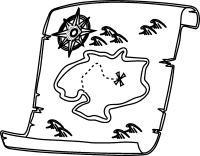
\includegraphics[height=40pt]{images/aneks-ref.png}}
                }{}%
            \ifsongproperty{music}{\\}{\ifsongproperty{annex}{\\}{}}%
            \ifsongproperty{lyrics}{%
                Tekst: \songproperty{lyrics} \\%
                }{}%
            \ifsongproperty{interpret}{%
                Interpretacja: \songproperty{interpret} \\%
                }{}%
            \ifsongproperty{capo}{%
                \capo{} \\%
                }{}%
        \end{tabular}%
        \par
    \endgroup
}

\setleadsheets{%
    title-template = custom,
    verse/numbered,
    remember-chords = false,
    align-chords = {l},
    capo-nr-format = arabic,
    bar-shortcuts
}
\setchords{%
    minor = {lowercase},
    input-notation = german,
    output-notation = german
}

\renewcommand{\chaptermark}[1]{\markboth{#1}{}}

\fancypagestyle{plain}{%
    \fancyhf{}
    \fancyhead[L]{Jakieś piosenki}
    \fancyfoot[LE,RO]{\Large\thepage}
}
\fancypagestyle{szanty}{%
    \pagestyle{plain}
    \fancyhead[R]{Szanty}
    \fancyfoot[LO]{
\includegraphics[height=45pt]{images/kolo.png}}
    \fancyfoot[RE]{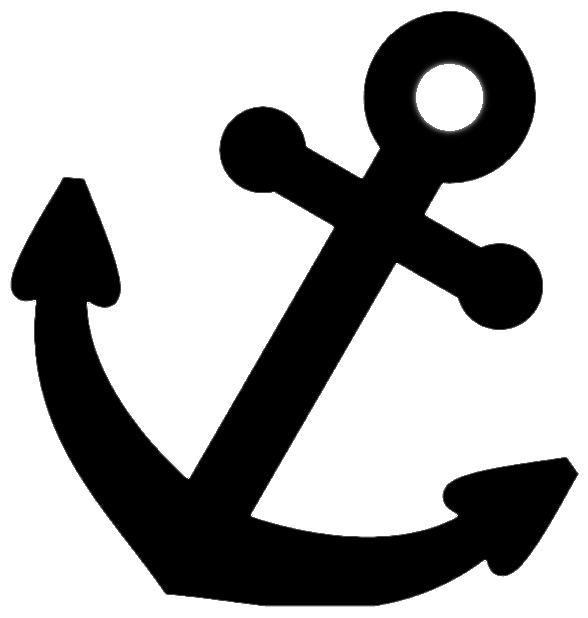
\includegraphics[height=45pt]{images/kotwica.png}}
}
\fancypagestyle{poezja}{%
    \pagestyle{plain}
    \fancyhead[R]{Poezja śpiewana}
    \fancyfoot[LO]{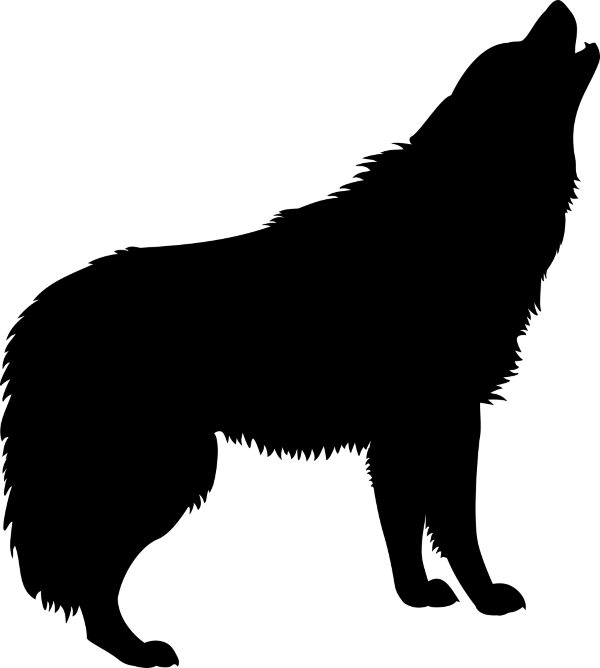
\includegraphics[height=45pt]{images/wilk.png}}
    \fancyfoot[RE]{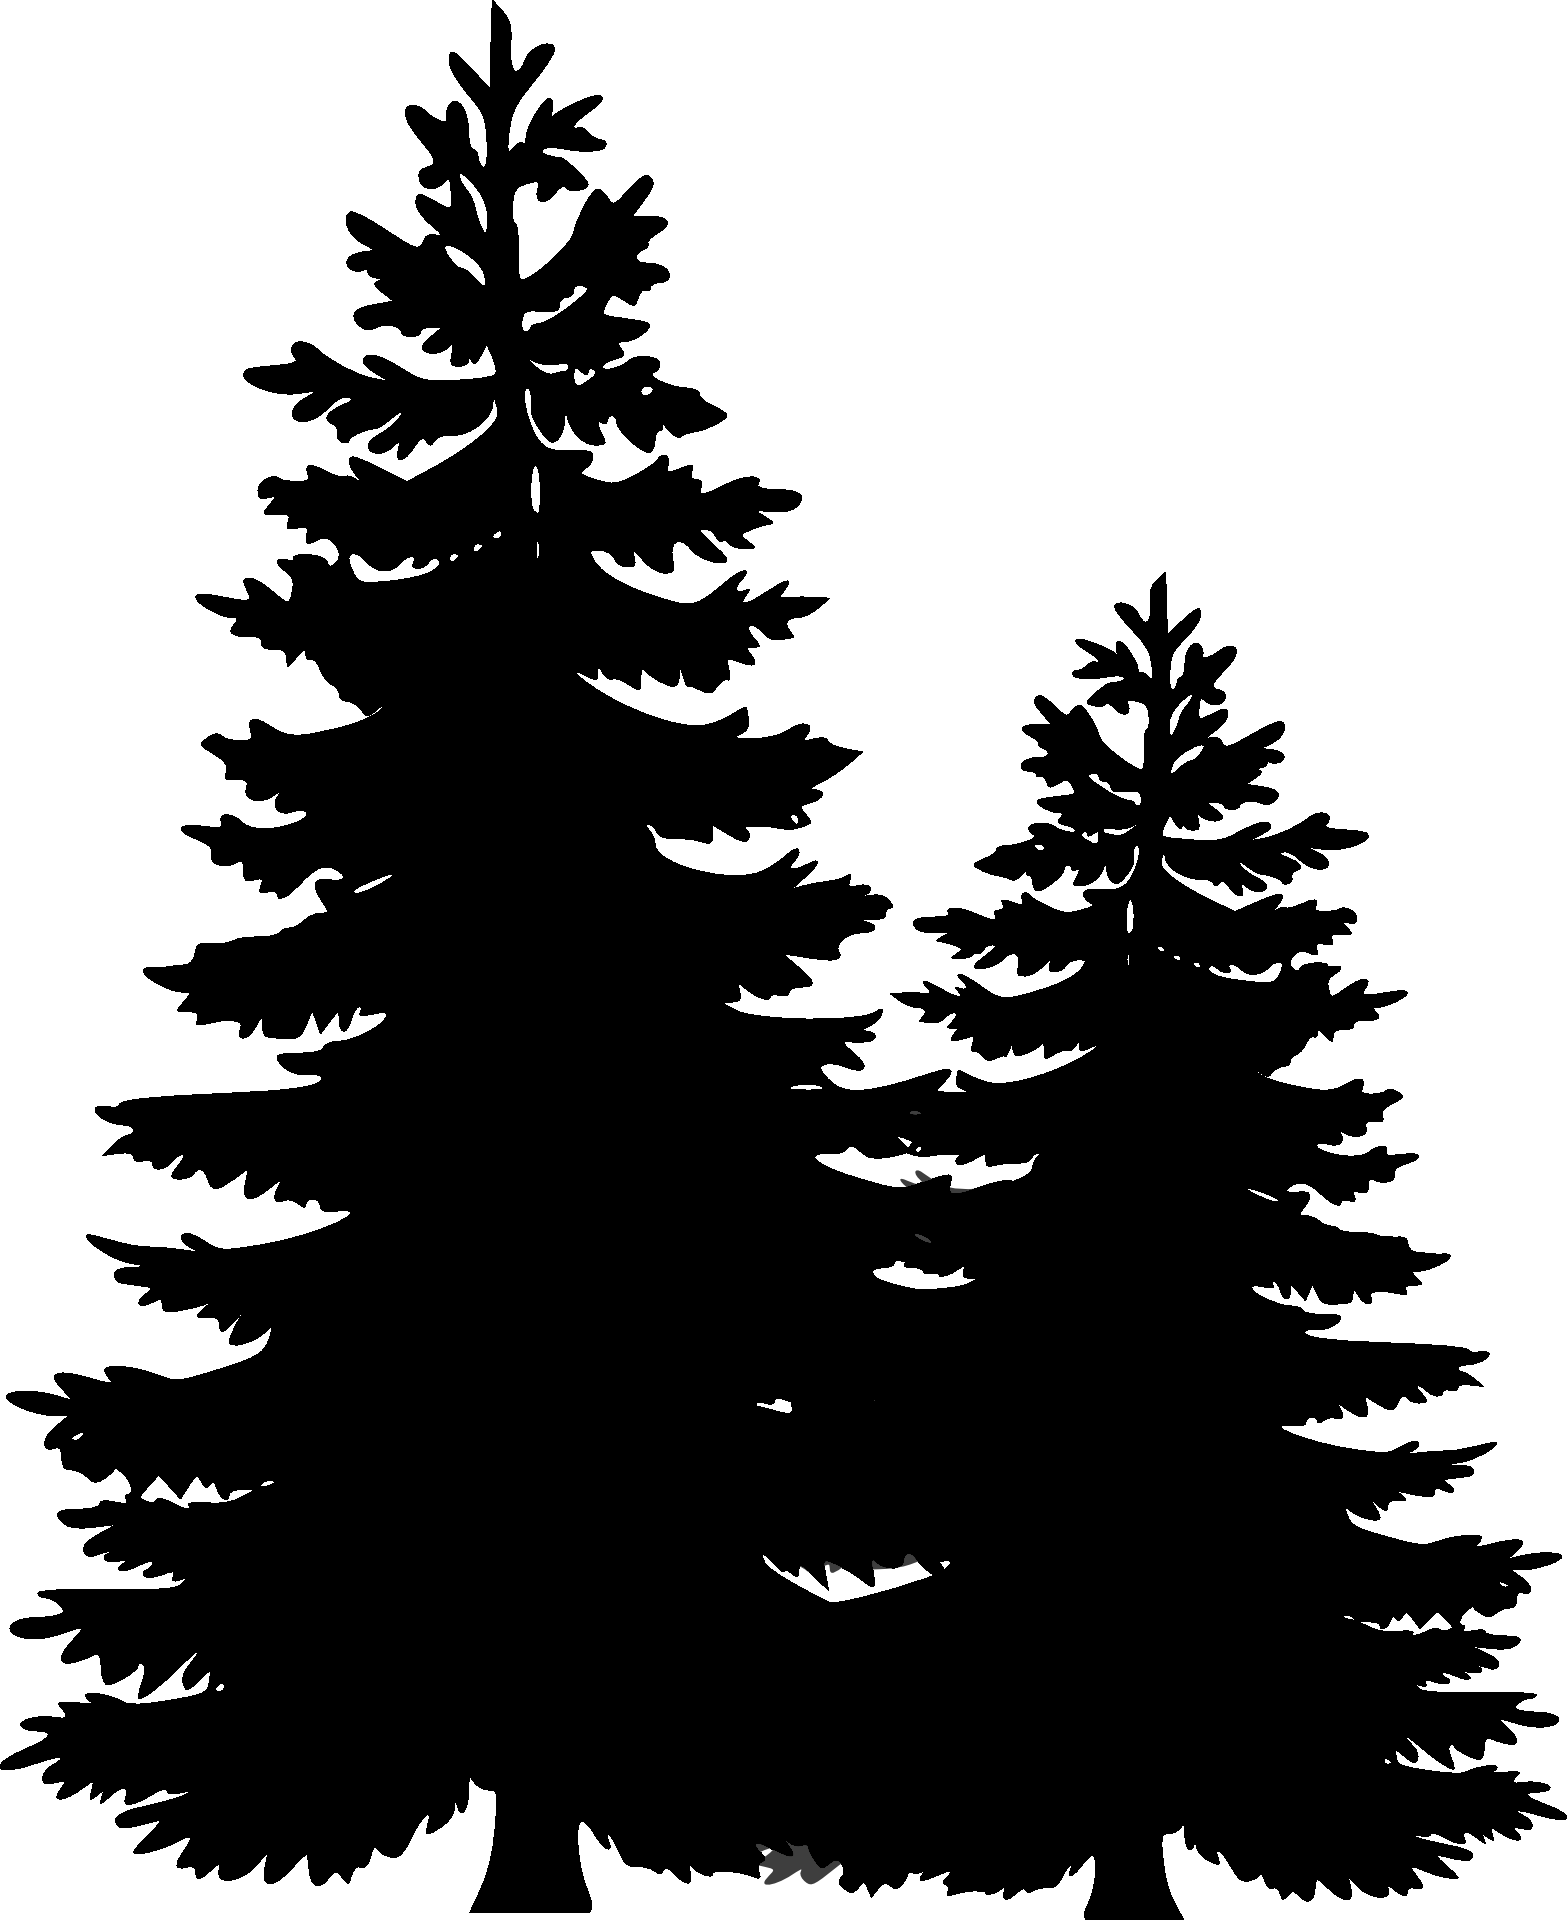
\includegraphics[height=45pt]{images/drzewa.png}}
}
\fancypagestyle{pop}{%
    \pagestyle{plain}
    \fancyhead[R]{Pop}
    \fancyfoot[LO]{
\includegraphics[height=45pt]{images/gwiazdy.png}}
    \fancyfoot[RE]{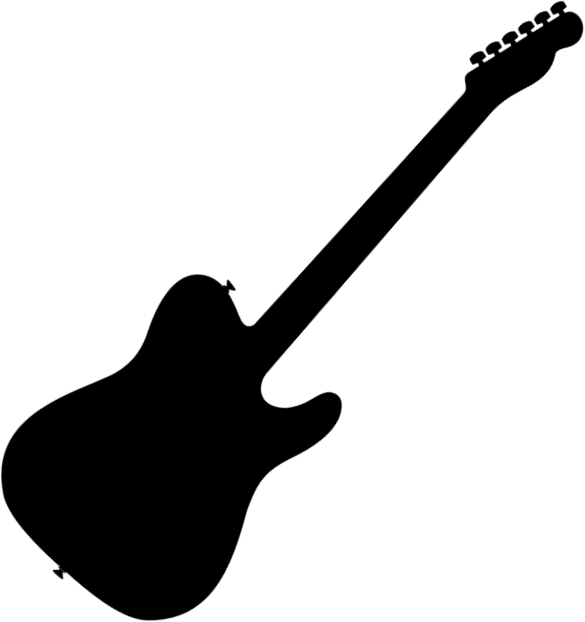
\includegraphics[height=45pt]{images/gitara.png}}
}
\fancypagestyle{autorskie}{%
    \pagestyle{plain}
    \fancyhead[R]{Autorskie}
    \fancyfoot[LO]{
\includegraphics[height=45pt]{images/kalamarz.jpeg}}
    \fancyfoot[RE]{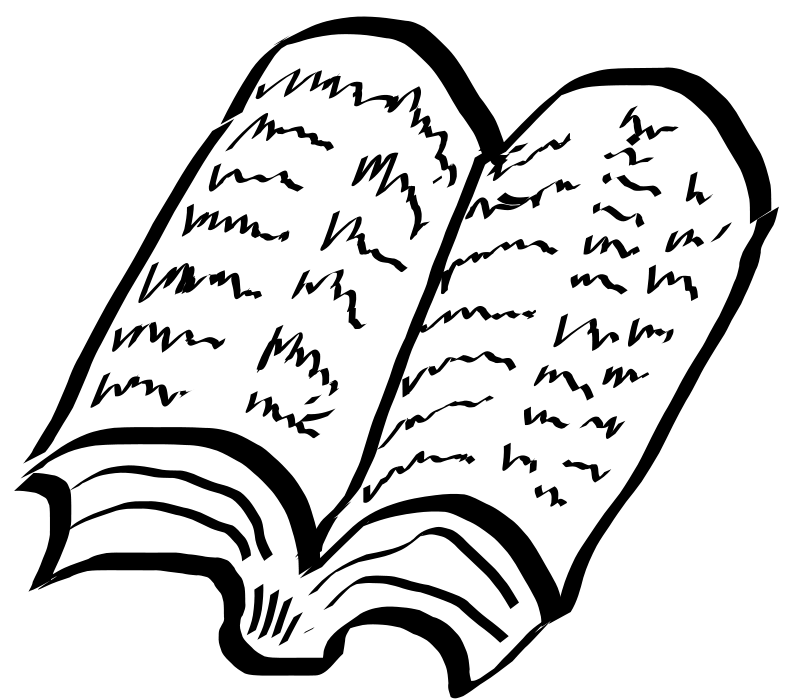
\includegraphics[height=45pt]{images/ksiazka_bazgroly.png}}
}
\fancypagestyle{legendy}{%
    \pagestyle{plain}
    \fancyhead[R]{Legendy, opowieści, ciekawostki}
    \fancyfoot[LO]{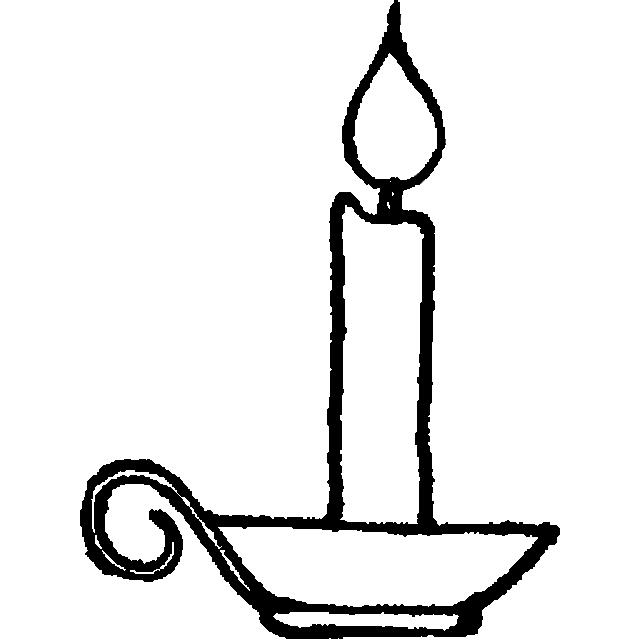
\includegraphics[height=45pt]{images/swieczka.png}}
    \fancyfoot[RE]{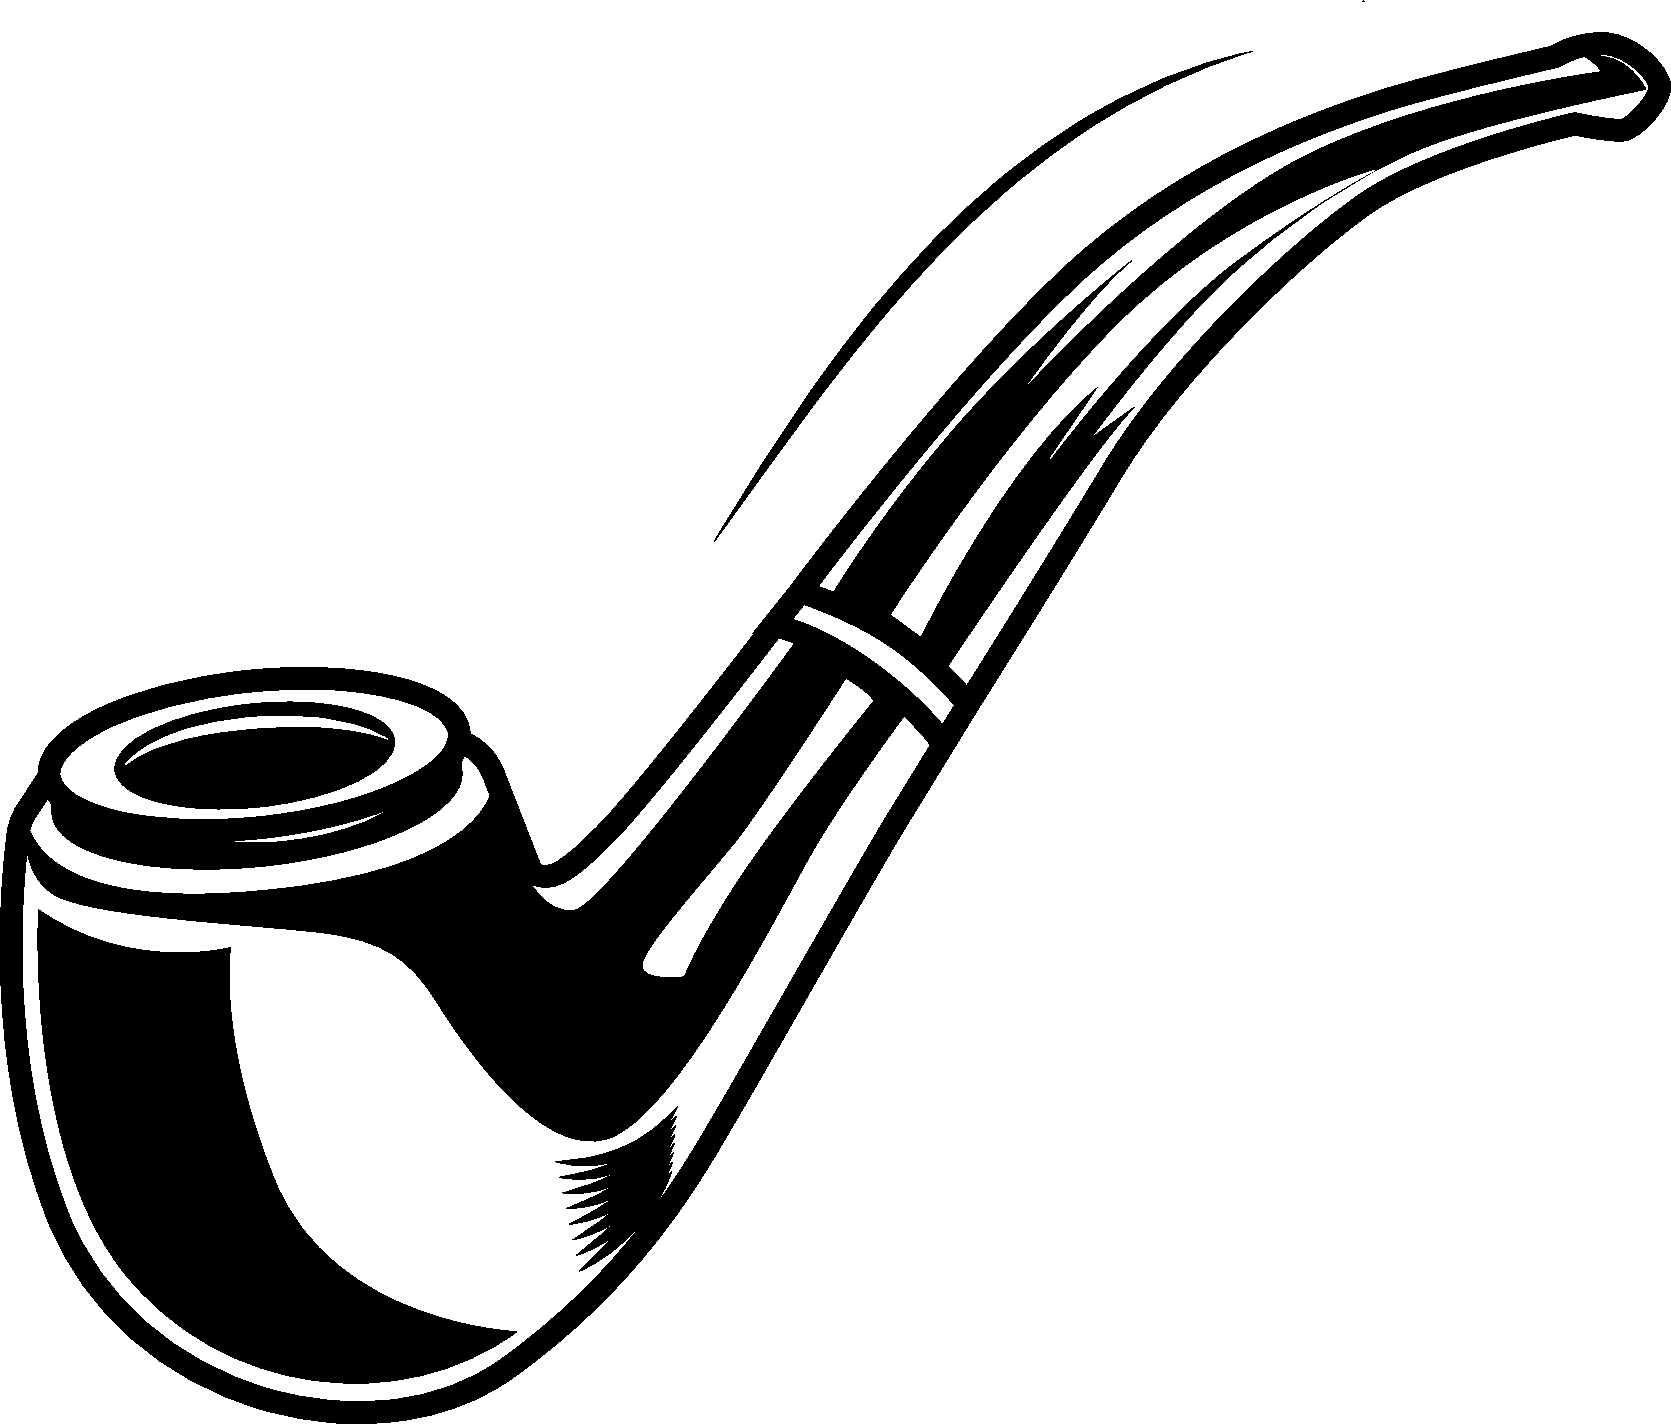
\includegraphics[height=45pt]{images/fajka.png}}
}

\renewcommand{\cftdot}{\ensuremath{\sim}}
\renewcommand{\cftsecleader}{\cftdotfill{\cftdotsep}}

% Usunięcie numeru rozdziału sprzed numeru sekcji
%\renewcommand{\thesection}{\arabic{section}}

\titleformat{\chapter}[block]{\centering\vspace{6cm}}{}{0pt}{\Huge\bfseries}

\newversetype{riff}[name={Riff}, numbered=false, named=true]

\counterwithin*{footnote}{section}

% Pionowy apostrof do angielskiego i francuskiego
\newcommand{\tqs}{\textquotesingle}

\begin{document}

\begin{titlepage}
    \begin{center}
        \vspace*{5cm}
        
        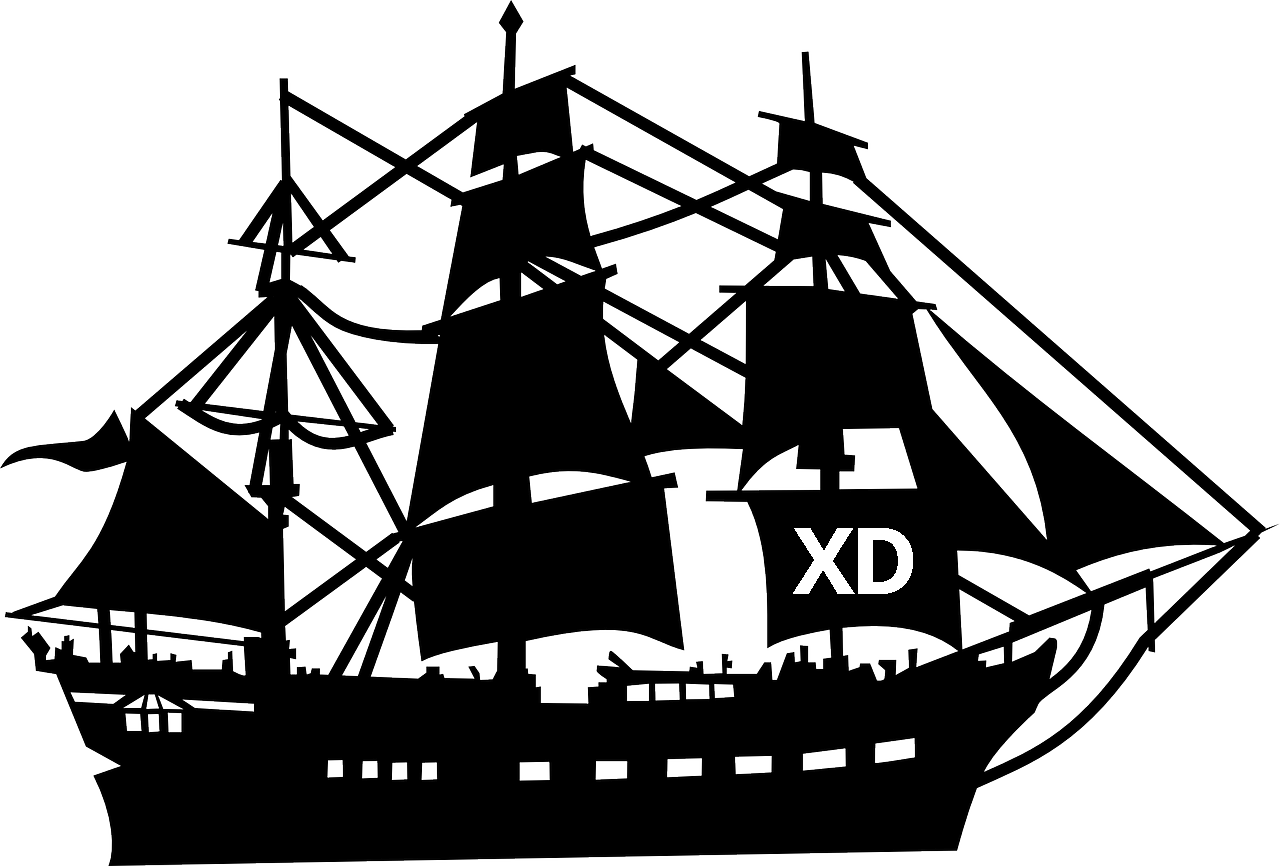
\includegraphics[height=8cm]{images/front-obrazek.png}

        \vspace{1.5cm}

        \Huge\textbf{Jakieś piosenki}
        
        \vspace{0.5cm}
        
        \large Wydanie pierwsze \\
        \small Podwydanie pierwsze
        
        \vfill

        \large
        Wydawnictwo Kis Inkris \\
        Warszawa, 2023

        \vspace{0.8cm}

        \footnotesize
        \textit{%
        Gdzie słyszysz śpiew, tam wejdź, tam dobre serce mają \\
        Żli ludzie, wierzaj mi, ci nigdy nie śpiewają} \medskip \\
        Johann Gottfried Seume, \textit{Die Gesänge}

    \end{center}
\end{titlepage}

\pagestyle{plain}

\tableofcontents
\vfill
\renewcommand{\tabularxcolumn}[1]{>{\small}b{#1}}
\begin{adjustbox}{width={\textwidth}, keepaspectratio}
\begin{tabularx}{\textwidth}{%
        @{}
        >{\raggedright\arraybackslash}X
        @{}
        >{\raggedleft\arraybackslash}X
    }
    \footnotesize
    Kamil Dzierżanowski \hfill opracowanie, skład, korekta

    Paweł Kulig \hfill opracowanie

    Piotr Wieżel \hfill opracowanie
    
    Mateusz Dorobek \hfill opracowanie

    \medskip

    Daj śpiewnikowi gwiazdkę na GitHubie:

    \smallskip

    \urlstyle{same}
    \url{https://github.com/dzierzanowski/spiewnik-szant}

    \bigskip

    Dziękujemy za grafiki z Freepik od dgim-studio i pch.vector!

    &

    Pobierz śpiewnik online:

    \smallskip

    
\includegraphics[width=3cm]{images/qr.png}
\end{tabularx}
\end{adjustbox}

\chapter{Szanty}
\begin{center}
    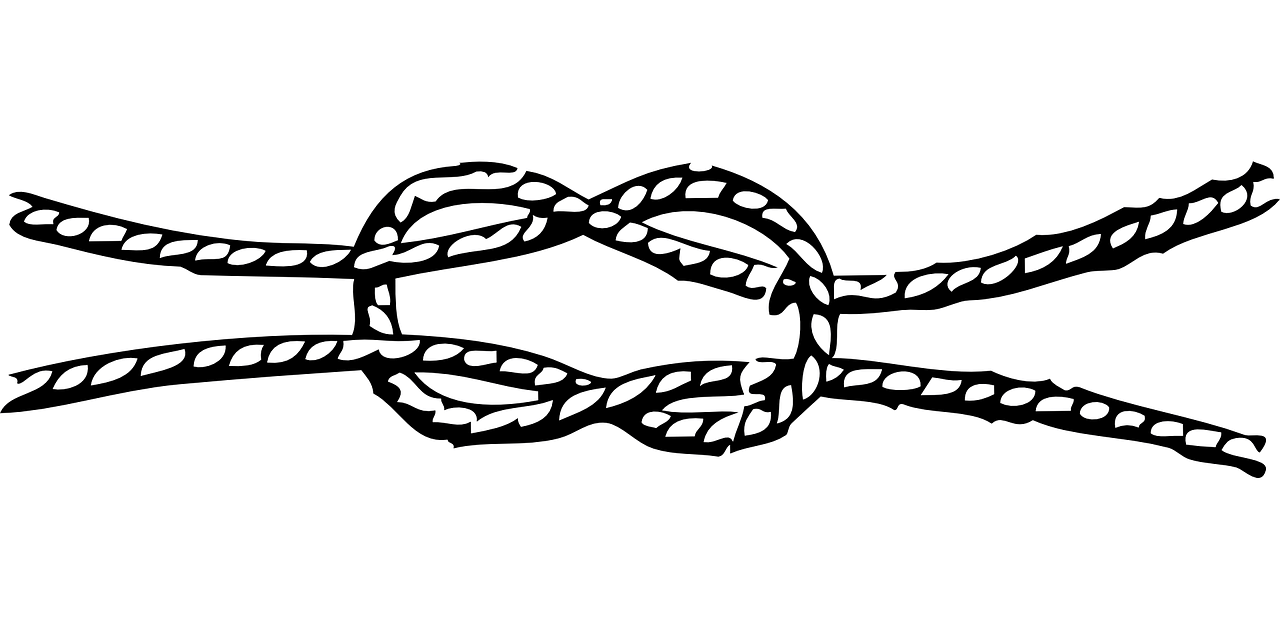
\includegraphics[width=0.5\textwidth]{images/wezel.png}
\end{center}
\pagestyle{szanty}
\newpage
\begin{song}{title={24 lutego (Bijatyka)}, interpret={Trzy Majtki}, music={tradycyjna}}
    \begin{verse}
        To dwu^{G}dziesty czwarty był lutego \\
        Po^{D}ranna zrzedła mgła \\
        A ^{e}wyszło z niej siedem uzbrojonych kryp \\
        Tu^{C}recki ^{D}niosły z^{e}nak
    \end{verse}
    \begin{chorus}
        No i z^{G}nów bijatyka, no i znów bijatyka \\
        No i bijatyka cały d^{D}zień \\
        I ^{e}porąbany dzień, i porąbany łeb \\
        Razem ^{C}bracia, ^{D}aż po z^{e}mierzch!
    \end{chorus}
    \begin{verse}
        I już pierwszy zbliża się do burt \\
        A zwie się \say{Goździk Lee} \\
        Z Algieru pasza wysłał go \\
        Żeby nam upuścił krwi
    \end{verse}
    \begin{chorus}
        No i znów bijatyka, no i znów bijatyka\ldots
    \end{chorus}
    \begin{verse}
        Już następny zbliża się do burt \\
        A zwie się \say{Róży Pąk} \\
        Plunęliśmy ze wszystkich luf \\
        Bardzo prędko szedł na dno
    \end{verse}
    \begin{chorus}
        No i znów bijatyka, no i znów bijatyka\ldots
    \end{chorus}
    \begin{verse}
        W naszych rękach dwa, i dwa na dnie \\
        Cała reszta zwiała gdzieś \\
        A jeden z nich zabraliśmy \\
        Aż na Starej Anglii brzeg
    \end{verse}
    \begin{chorus}
        No i znów bijatyka, no i znów bijatyka\ldots
    \end{chorus}
\end{song}


\newpage
\begin{song}{title={Bitwa}, music={Mechanicy Shanty}}
\begin{multicols}{2}
    \begin{intro}
        e h C a \\
        e D e e
    \end{intro}
    \begin{verse}
        ^{e}Okręt nasz w^{h}płynął w mgłę ^{C}i fregaty d^{a}wie \\
        Popłyn^{e}ęły ^{D}naszym kursem ^{G}by nie zgubić s^{H7}ię \\
        ^{e}Potem szkwał w^{h}ypchnął nas ^{C}poza mleczny ^{a}pas \\
        I nikt wt^{e}edy n^{D}ie przypuszczał, ^{G}że fregaty ^{H7}śmierć nam niosą
    \end{verse}
    \begin{chorus}
        ^{G}Ciepła kr^{D}ew poleje ^{e}się strug^{h}ami \\ 
        ^{C}Wygra ten, k^{a}to utrz^{D}yma ^{e}ship \\
        W ^{G}huku dział ^{D}ktoś przykryje ^{e}się fal^{h}ami \\
        ^{C}Jak da Bóg, ^*{a}ocal ^{D}imy ^{e}bryg
    \end{chorus}
    \begin{verse}
        Nagły huk w uszach grał i już atak trwał \\
        To fregaty uzbrojone rzędem w setkę dział \\
        Czarny dym spowił nas, przyszedł śmierci czas \\
        Krzyk i lament mych kamratów, przerywany ogniem katów
    \end{verse}
    \begin{chorus}
        Ciepła krew poleje się strugami\ldots
    \end{chorus}
    \begin{verse}
        Pocisk nasz trafił w maszt, usłyszałem trzask \\
        To sterburtę rozwaliła jedna z naszych salw \\
        "Żagiel staw" krzyknął ktoś, znów piratów złość \\
        Bo od rufy nam powiało, a fregatom w mordę wiało
    \end{verse}
    \begin{chorus}
        Ciepła krew poleje się strugami\ldots
    \end{chorus}
    \begin{verse}
        Z fregat dwóch tylko ta pierwsza w pogoń szła \\
        Wnet abordaż rozpoczęli, gdy dopadli nas \\
        Szyper ich dziury dwie zrobił w swoim dnie \\
        Nie pomogło to psubratom, reszta z rei zwisa za to
    \end{verse}
    \begin{chorus}
        Ciepła krew poleje się strugami\ldots
    \end{chorus}
    \begin{verse}
        Po dziś dzień tamtą mgłę i fregaty dwie \\
        Kiedy noc zamyka oczy, widzę w moim śnie \\
        Tamci, co śpią na dnie, uśmiechają się \\
        Że ich straszną śmierć pomścili bracia, którzy zwyciężyli
    \end{verse}
    \begin{chorus}
        Ciepła krew poleje się strugami\ldots
    \end{chorus}
\end{multicols}
\end{song}


\newpage
\begin{song}{title={Chłopcy z Botany Bay}, music={Mietek Folk}, capo=3}
\begin{multicols}{2}
    \begin{verse}
        Już nad ^{h}Hornem ^{A}zapada ^{h}noc ^{h} \\
        Wiatr na ^{h}żaglach ^{A}położył ^{D}się ^{D} \\
        |: A tam ^{G}jeszcze ^{A}korsarze na ^*{D}Bota ^{A}ny ^{h}Bay | \\
        | Upy^{G}chają ^{A}zdobycze ^{h}swe :|
    \end{verse}
    \begin{verse}
        Jolly Roger na maszcie już śpi \\
        Jutro przyjdzie z Hiszpanem się bić \\
        A korsarze znużeni na Botany Bay \\
        Za zwycięstwo dziś będa swe pić
    \end{verse}
    \begin{verse}
        Śniady Clark puchar wznosi do ust \\
        "Bracia, toast! Niech idzie na dno!" \\
        Tylko Johnny nie pije, bo kilka mil stąd \\
        Otuliło złe morze go
    \end{verse}
    \begin{verse}
        Nie podnosi kielicha do ust \\
        Zawsze on tu najgłośniej się śmiał \\
        Mistrz fechtunku z Florencji ugodził go \\
        Już nie będzie za szoty się brał
    \end{verse}
    \begin{verse}
        W starym porcie zapłacze Margot \\
        Jej kochany nie wróci już \\
        Za dezercję do panny na kei w Brisbane \\
        Oddać musiał swą głowę pod nóż
    \end{verse}
    \begin{verse}
        Tak niewielu zostało dziś ich \\
        Resztę zabrał Neptun pod dach \\
        Choć na ustach wciąż uśmiech, to w sercach lód \\
        W kuflu miesza się rum i strach
    \end{verse}
    \begin{verse}
        To ostatni chyba już rejs \\
        Cios sztyletem lub kula w pierś \\
        Bóg na szkuner w niebiosach zabierze ich \\
        Wszystkich chłopców z Botany Bay
    \end{verse}
    \begin{verse}
        Już nad Hornem zapada noc \\
        Wiatr na żaglach położył się \\
        A tam jeszcze korsarze na Botany Bay \\
        Upychają zdobycze swe
    \end{verse}
\end{multicols}
\end{song}


\newpage
\begin{song}{title={Cztery piwka}, interpret={Trzy Majtki}, music={Jerzy Porębski}}
    \small
    \begin{verse}
        ^{g}Ze Świnoujścia do Walvis Bay droga nie była krótka \\
        A ^{g}po dwóch dobach (albo mniej) j^{D}uż się skończyła w^{g}ódka \\
        \say{Do b^{g}rydża!} --- krzyknął Siwy Flak i z miejsca rzekł: \say{Dwa piki} \\
        A ^{g}ochmistrz w \say{telewizor} wlał nie ^{D}byle jakie ^{G}siki
    \end{verse}
    \begin{chorus}
        Cztery ^{G}piwka na stół, w ^{C}popielniczkę pet \\
        J^{D}akąś damę roześmianą król przytuli wn^{G}et \\
        G^{G}dzieś między palcami ^{C}sennie płynie czas \\
        Cz^{D}warta ręka króla bije as ^{g}
    \end{chorus}
    \begin{verse}
        A w karcie tylko jeden as i nic poza tym nie ma \\
        Ale nie powiem przecie \say{pas}, może zagrają szlema \\
        \say{Kontra} --- mu rzekłem, taki blef, by nieco spuścił z tonu \\
        A Fred mi na to: \say{Cztery trefl!} --- przywalił bez pardonu
    \end{verse}
    \begin{chorus}
        Cztery piwka na stół, w popielniczkę pet\ldots
    \end{chorus}
    \begin{verse}
        A mój w dwa palce obtarł nos, to znaczy: \say{Nie mam nic} \\
        I wtedy Flak, podnosząc głos, powiedział: \say{Cztery pik!} \\
        I kiedy jeszcze cztery króle pokazał mu jak trza \\
        To Fred z renonsem: \say{Siedem pik!} powiedział, \say{niech gra Flak!}
    \end{verse}
    \begin{chorus}
        Cztery piwka na stół, w popielniczkę pet\ldots
    \end{chorus}
    \begin{verse}
        A ja mu \say{kontra}, on mi \say{re}, ja czuję pełen luz \\
        Bo widzę w moich kartach, że jest atutowy tuz \\
        Więc strzelam! Kiedy karty Fred wyłożył mu na blat \\
        To każdy mógł zobaczyć, jak Siwego Flaka trafia szlag
    \end{verse}
    \begin{chorus}
        Cztery piwka na stół, w popielniczkę pet\ldots
    \end{chorus}
    \begin{verse}
        Już nie pamiętam, ile dni w miesiące złożył czas \\
        Morszczuki dosyć dobrze szły i grało się nieraz \\
        Lecz nigdy więcej Siwy Flak, klnę na jumprowe wszy\footnote{potoczna nazwa na odstające druciki w stalowych linach, które powodują swędzące rany na dłoniach} \\
        Choć byś go prosił, tak czy siak, nie zasiadł już do gry
    \end{verse}
    \begin{chorus}
        W popielniczkę pet, cztery piwka na stół \\
        Już tej damy roześmianej nie przytuli król \\
        Gdzieś nam się zapodział atutowy as \\
        Tego szlema z nami wygrał czas
    \end{chorus}
\end{song}


\newpage
\begin{song}{title={Dziesięć w skali Beauforta}, music={Krzysztof Klenczon}, capo=3, annex}
    \begin{multicols}{2}
    \begin{verse}
        Ko^{e}łysał nas zac^{a}hodni wiatr \\
        ^{H7}Brzeg gdzieś za rufą z^{e}ostał \\
        I n^{a}agle ktoś jak p^{e}apier zbladł \\
        ^{F#7}Sztorm idzie, panie ^{H}bosman
    \end{verse}
    \begin{chorus}
        A ^*{C}bo sm^{G}an tylko ^{C}zapiął pł^{G}aszcz \\
        I z^{C}aklął: \say{^{H7}Ech, do cz^{e}orta \\
        Nie da^{C}ję ła^{D}jbie ż^{G}adnych s^{e}zans} \\
        ^{e}Dziesięć w ^{a}skali ^*{H7}Beau ^{e}forta
    \end{chorus}
    \vfill\null\columnbreak{}
    \begin{verse}
        Z zasłony ołowianych chmur \\
        Ulewa spadła nagle \\
        Rzucało nami w górę, w dół \\
        I fala zmyła żagle
    \end{verse}
    \begin{chorus}
        A bosman tylko zapiął płaszcz\ldots
    \end{chorus}
    \begin{verse}
        Gdzie został ciepły, cichy kąt \\
        I brzegu kształt znajomy \\
        Zasnuły mgły daleki ląd \\
        Dokładnie, z każdej strony
    \end{verse}
    \begin{chorus}
        A bosman tylko zapiął płaszcz\ldots
    \end{chorus}
    \begin{verse}
        O pokład znów uderzył deszcz \\
        I padał już do rana \\
        Piekielnie ciężki to był rejs \\
        Szczególnie dla bosmana
    \end{verse}
    \begin{chorus}
        A bosman tylko zapiął płaszcz \\
        I zaklął: \say{Ech, do czorta \\
        Przedziwne czasem sny się ma} \\
        Dziesięć w skali Beauforta \medskip \\
        Dziesięć w skali Beauforta \\
        Dziesięć w skali Beauforta
    \end{chorus}
    \end{multicols}
\end{song}


\newpage
\begin{song}{title={Few days}, music={Ryczące Dwudziestki}, annex}
\begin{multicols}{2}
    \begin{verse}
        O Panie, czemu w ziemi tkwię \\
        Hej raz, hej raz! \\
        I macham szuflą cały dzień? \\
        Hej, na morze czas!
    \end{verse}
    \begin{chorus}
        Mogę kopać tu dalej \\
        Few days, few days \\
        Mogę kopać przez dni parę \\
        Ale wracać chcę $\times 2$
    \end{chorus}
    \begin{verse}
        Tam każdy takie bajdy plótł \\
        Nie raz, nie raz \\
        Przekroczysz Jukon, złota w bród \\
        Hej, na morze czas!
    \end{verse}
    \begin{chorus}
        Mogę kopać tu dalej\ldots $\times 2$ 
    \end{chorus}
    \vfill\null\columnbreak{}
    \begin{verse}
        Wykopię jeszcze parę dziur \\
        Hej raz, hej raz \\
        Wytoczę płonnej skały wór \\
        Hej, na morze czas!
    \end{verse}
    \begin{chorus}
        Mogę kopać tu dalej\ldots $\times 2$ 
    \end{chorus}
    \begin{verse}
        Za żonę tu łopatę mam \\
        Już dość, już dość \\
        A zysk, że jej uzywam sam \\
        Hej, na morze czas!
    \end{verse}
    \begin{chorus}
        Mogę kopać tu dalej\ldots $\times 2$
    \end{chorus}
    \begin{verse}
        O Panie nie jest to Twój raj \\
        O nie, o nie \\
        Nadzieję innym głupcom daj \\
        Ja na morze chcę!
    \end{verse}
    \begin{chorus}
        Chociaż już mi wystarczy \\
        Few days, few days \\
        Dam Ci jeszcze jedną szansę \\
        Ale wracać chcę $\times 2$
    \end{chorus}
\end{multicols}
\end{song}


\newpage
\begin{song}{title={Gdzie ta keja}, music={Jerzy Porębski}, interpret={Trzy Majtki}}
    \begin{verse}
        Gdyby ^{a}tak ktoś przyszedł i powiedział: \say{S^{E}tary, czy masz ^{a}czas? \\
        Potrze^{C}buję do załogi j^{G}akąś nową t^{C}warz \\
        Ama^{C}zonka, Wielka R^{C7}afa, ^{d} oceany trzy \\
        Rejs na ^{a}całość, rok, dwa lata} --- ^{E}to powiedział^{a}bym:
    \end{verse}
  	\begin{chorus}
        Gdzie ta ^{a}keja, a ^{E}przy niej ten j^{a}acht \\
        Gdzie ta ^{C}koja, ^{G}wymarzona w s^{C}nach \\
        Gdzie te w^{g}szystkie sz^{A7}nurki ^{d}od ^{A7}tych sz^{d}mat \\
        Gdzie ta b^{a}rama ^{E}na szeroki ś^{a}wiat
    \end{chorus}
    \begin{chorus*}
        Gdzie ta keja, a przy niej ten jacht \\
        Gdzie ta koja wymarzona w snach \\
        W każdej chwili płynę w taki rejs \\
        Tylko gdzie to jest, no gdzie to jest
    \end{chorus*}
    \begin{verse}
        Gdzieś na dnie wielkiej szafy leży ostry nóż \\
        Stare jeansy wystrzępione impregnuje kurz \\
        W kompasie igła zardzewiała, lecz kierunek znam \\
        Biorę wór na plecy i przed siebie gnam
    \end{verse}
  	\begin{chorus}
        Gdzie ta keja, a przy niej ten jacht\ldots
    \end{chorus}
    \begin{verse}
        Przeszły lata zapyziałe, rzęsą zarósł staw \\
        A na przystani czółno stało --- kolorowy paw \\
        Zaokrągliły się marzenia, wyjałowiał step \\
        Lecz dalej marzy o załodze ten samotny łeb
    \end{verse}
  	\begin{chorus}
        Gdzie ta keja, a przy niej ten jacht\ldots
    \end{chorus}
\end{song}


\newpage
\fancyfoot[LO,RE]{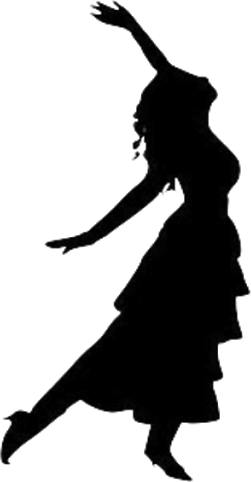
\includegraphics[height=45pt]{images/hiszpanska-dziewczyna.png}}
\begin{song}{title={Hiszpańskie dziewczyny}, music={tradycyjna angielska (Spanish Ladies)}, lyrics={Ryczące Dwudziestki}, capo={2}, annex}
    \begin{intro}
        Żegnajcie nam dziś, hiszpańskie dziewczyny \\
        Żegnajcie nam dziś, marzenia ze snów \\
        Ku brzegom angielskim już rzuszać nam pora \\
        Lecz kiedyś na pewno wró^{F#7}cimy tu z^{h}nów
    \end{intro}
    \begin{chorus}
        I s^{h}mak waszych ust, hiszpańskie dziew^{f#}czyny \\
        W noc ^{h}ciemną i złą nam będzie się ^{A}śnił \\
        Le^{G}niwie pop^{A}łyną znów ^{D}rejsu go^{h}dziny \\
        Wspom^{G}nienie ust waszych przys^{F#7}porzy nam ^{h}sił $\times 2$
    \end{chorus}
    \begin{verse}
        Nie^{h}długo ujrzymy znów w dali Cape ^*{f#}Dead man\footnotemark{} \\
        I Gł^{h}owę Baranią\footnotemark{} sterczącą wśród wz^{A}górz \\
        I s^{G}tatki sto^{A}jące na ^{D}redzie przed ^{h}Plymouth \\
        Kla^{G}rować kotwicę naj^{F#7}wyższy czas ^{h}już
    \end{verse}
    \begin{chorus}
        I smak waszych ust, hiszpańskie dziewczyny\ldots $\times 2$
    \end{chorus}
    \begin{verse}
        I znów białe żagle na masztach rozkwitną \\
        Kurs szyper wyznaczy do Portland i Wight\footnotemark{} \\
        I znów stara łajba potoczy się ciężko \\
        Przez fale, w kierunku na Beachy, Fairlight\footnotemark{}
    \end{verse}
    \begin{chorus}
        I smak waszych ust, hiszpańskie dziewczyny\ldots $\times 2$
    \end{chorus}
    \begin{verse}
        Zabłysną nam bielą skał zęby pod Dover \\
        I znów noc w kubryku wśród legend i bajd \\
        Powoli i znojnie tak płynie nam życie \\
        Na wodach i w portach South Foreland Light\footnotemark{}
    \end{verse}
    \begin{chorus}
        I smak waszych ust, hiszpańskie dziewczyny\ldots $\times 2$
    \end{chorus}
    \footnotetext{Dodman Point, Kornwalia; nie mylić z Cape Diamond, Quebec City --- to po innej stronie oceanu}
    \footnotetext{Ram Head, Kornwalia}
    \footnotetext{Isle of Wight (\textipa{/waIt/})}
    \footnotetext{Beachy Head i Fairlight, East Sussex}
    \footnotetext{wiktoriańska latarnia morska w South Foreland, Kent; nie ustalono, co autor miał na myśli}
\end{song}

\newpage\pagestyle{szanty}
\newpage
\begin{song}{title={Jasnowłosa}, lyrics={Ryczące Dwudziestki}}
    \begin{verse}
        Na ^{G}tańcach ją poznałem, długo^*{C}wło ^{D}są ^{G}blond \\
        Dziew^{G}czynę moich ^{e}marzeń, nie wia^{C}domo ^{D}skąd \\
        ^{G}Ona się tam ^{e}wzięła, piękna ^{C}niczym ^*{F}kwia ^{D7}t \\
        Czy jak sy^{G}rena wyszła z morza, czy ją ^*{C}przy ^{D}gnał ^{G}wiatr?
    \end{verse}
    \begin{chorus}
        ^{G}Żegnaj, Irlandio, czas w ^{C}drogę ^{D} mi ^{G}już \\
        W ^{G}porcie go^{e}towa stoi ^{C}moja ^{D}łódź \\
        Na ^{G}wielki o^{e}cean przyjdzie ^{C}mi zaraz ^*{F}wy ^{D7}jść \\
        I po^{G}żegnać się z dziewczyną na ^*{C}Loughin ^*{D}sho ^{G}lin
    \end{chorus}
    \begin{verse}
        Ująłem ją za rękę delikatną, jak \\
        Latem mały motyl albo róży kwiat \\
        Poszedłem z nią na plażę, wsłuchać się w szum fal \\
        Pokazałem jasnowłosej wielki morza czar
    \end{verse}
    \begin{chorus}
        Żegnaj, Irlandio, czas w drogę mi już\ldots
    \end{chorus}
    \begin{verse}
        Za moment wypływam w długi, trudy rejs \\
        I z piękną mą dziewczyną przyjdzie rozstać się \\
        Żagle pójdą w górę, wiatr mnie pogna w przód \\
        I przez morza mnie powiedzie, ty zostaniesz tu
    \end{verse}
    \begin{chorus}
        Żegnaj, Irlandio, czas w drogę mi już\ldots $\times 2$
    \end{chorus}
\end{song}


\newpage
\begin{song}{title={Ja stawiam}, music={EKT Gdynia}}
    \begin{verse}
        Czy ^{e}mam pieniądze, czy g^{D}rosza mi brak, ja s^{e}tawiam (ja stawiam!) \\
        Czy ^{e}los mi sprzyja, czy ^{D}idzie mi wspak, ja s^{e}tawiam (ja stawiam!) \\
        |: Czy m^{e}am kompanów dzie^{G}sieciu, czy dwóch \\
        Czy m^{A}am ochotę na r^{C}um, czy na mi^{H7}ód \\
        Czy ^{e}mam pieniądze, czy g^{D}rosza mi brak, ja s^{e}tawiam :|
    \end{verse}
    \begin{verse}
        Czy wicher w oczy, czy w plecy mi dmie, ja stawiam \\
        Czy mi kompani ufają, czy nie, ja stawiam \\
        Czy ja ścigam wroga, czy wróg ściga mnie \\
        Dopóki mój okręt nie leży na dnie \\
        Czy wicher w oczy, czy w plecy mi dmie, ja stawiam
    \end{verse}
    \begin{solo}
        \textit{(opcjonalnie tutaj)}
    \end{solo}
    \begin{verse}
        A kiedy mnie dziewka porzuci jak psa, ja stawiam \\
        Gąsiorek biorę i piję do dna, ja stawiam \\
        Kompanię zbieram i siadam za stół \\
        Nie ma wtedy płacenia na pół! \\
        Bo kiedy mnie dziewka porzuci jak psa, ja stawiam
    \end{verse}
    \begin{verse}
        Ja stawiam żagiel jak kufel na stół, ja stawiam \\
        Czy fala mnie niesie w górę, czy w dół, ja stawiam \\
        Czy tam dopłynę, gdzie kończy się świat \\
        Czy aż do piekła poniesie mnie wiatr \\
        Ja stawiam żagiel jak kufel na stół, ja stawiam \medskip \\
        Ja stawiam żagiel jak kufel na stół, ja stawiam \\
        Ja stawiam żagiel jak kufel na stół, ja stawiam
    \end{verse}
\end{song}


\newpage
\begin{song}{title={Kapitan Kidd}, music={North Cape}}
\begin{multicols}{2}
    \begin{chorus}
        Me ^{e}imię ^{h}William ^{e}Kidd \\
        Już czeka ^{a}stryk, czeka ^{D}stryk \\
        Królewski ^{e}korsarz ^{h}William ^{e}Kidd, czeka ^*{G}stry ^{D}k \\
        Me ^{G}imię ^{D}William ^{a}Kidd \\
        Zbrodni ^*{e}ogrom ^{h}nych to ^{a}mit \\
        Powró^{e}ciłem, ^{G}choć w Lon^{h}dynie ^{D/F#}czeka ^{e}stryk
    \end{chorus}
    \begin{verse}
        Mój ^{e}ojciec ^{h}uczył ^{e}mnie \\
        Jak nie ^{G}znaleźć się na ^{D}dnie \\
        Lecz los o^{e}krutny ^{D}zabrał ^{a}go ro^{h}dzinie ^{e}mej \\
        Choć biblię w ^{e}rękę ^{h}moją ^{e}kładł \\
        Morza ^{G}urok na mnie ^{D}padł \\
        I mary^{e}narzem ^{D}stałem ^{a}się, choć ^{h}czeka ^{e}stryk
    \end{verse}
    \begin{chorus}
        Me imię William Kidd\ldots
    \end{chorus}
    \begin{verse}
        Kanonier William Moore \\
        Pierwszy trafił na mój sznur \\
        Bo przeciw mnie ośmielił się on wzniecić bunt \\
        Choć dobrym strzelcem William był \\
        Pod salingiem będzie gnił \\
        Buntownik każdy skończy tak, już czeka stryk
    \end{verse}
    \begin{chorus}
        Me imię William Kidd\ldots
    \end{chorus}
    \begin{verse}
        Raz gdy było ze mną źle \\
        Obiecałem sobie, że \\
        Mądrości drogą odtąd pójdę po kres dni \\
        Lecz mój korsarski podły fach \\
        Zabił wnet o duszę strach \\
        I potępienie czeka mnie, bo czeka stryk
    \end{verse}
    \begin{chorus}
        Me imię William Kidd\ldots
    \end{chorus}
    \begin{verse}
        \textit{(wolniej)} \\
        To egzekucyjny blok \\
        Zaraz mnie ogarnie mrok \\
        Bo na mą szyję kat założy gruby sznur \\
        Więc dzisiaj ostrzec ciebie chcę \\
        Byś za przykład nie brał mnie \\
        Mądrości drogą zawsze szedł, bo czeka stryk
    \end{verse}
    \begin{chorus}
        \textit{(szybciej)} \\
        Me imię William Kidd\ldots
    \end{chorus}
\end{multicols}
\end{song}
\newpage

\newpage
\begin{song}{title={La Valette}, interpret={Perły i Łotry}, music={tradycyjna (Le Loup, le Renard et la Belette)}, capo=3, annex}
    \begin{intro}
        Hej, ho! brakuje oregano! \smallskip \\
        \writechord{G} \writechord{A}
    \end{intro}
    \begin{multicols}{2}
    \begin{chorus}
        ^{e}Pierwszy raz, kiedym stanął w La Valette \\
        ^{G}Bitwy smak poczuły ^{A}usta me \smallskip \\
        Pierwszy raz, kiedym stanął w La Valette \\
        Bitwy smak poczuły usta me \smallskip \\
        Na ^{e}prawo bić, na lewo lać \\
        ^{G}Na kolana Anglio, ^{A}dzisiaj Francji czas \smallskip \\
        Na prawo bić, na lewo lać \\
        Na kolana Anglio, dzisiaj Francji czas $\times 2$
    \end{chorus}
    \smallskip
    \begin{verse}
        Z ^{e}morza widzę Malty brzeg \\
        ^{A}Zbliża się wyzwanie \\
        W ^{e}gardłach armat lont już wrze \\
        ^{A}Kończyć ładowanie! \smallskip \\
        ^{e}Niespokojna żagli biel \\
        ^{A}Trzy kolowy flagi \\
        ^{e}Dalej bracia, równać cel \\
        ^{A}Król zostanie nagi!
    \end{verse}
    \smallskip
    \begin{chorus}
        Pierwszy raz, kiedym stanął w La Valette\ldots $\times 2$
    \end{chorus}
    \vfill\null\columnbreak{}
    \begin{verse}
        Zaraz padnie pierwszy strzał \\
        Już się wiara zbroi \\
        Każdy z nas tej bitwy chciał \\
        Dalej, bić Angoli! \smallskip \\
        Kapitana groźny wzrok \\
        Gromki krzyk załogi \\
        Zaraz zrobi pierwszy krok \\
        \textit{« Vive la France ! »} przeraża wrogów
    \end{verse}
    \begin{interlude}
        \textit{(akordy jak w refrenie)} \\
        \textit{(solo na banjo, jeżeli ktoś ma banjo)}
    \end{interlude}
    \begin{chorus}
        Pierwszy raz, kiedym stanął w La Valette\ldots
    \end{chorus}
    \begin{verse}
        Zapach prochu, błyski szpad \\
        W słońcu lśni fregata \\
        Pierwszy pocisk obok spadł \\
        Dalej, bić psubrata! \smallskip \\
        Dla Francuzów idziem w bój \\
        Za wolności śladem \\
        Trzy kolory to nasz strój \\
        Trzęsie Angol zadem
    \end{verse}
    \begin{chorus}
        Pierwszy raz, kiedym stanął w La Valette\ldots $\times 4$
    \end{chorus}
    \begin{outro}
        Hej, ho! brakuje oregano! \\
        \writechord{G} \writechord{A} \writechord{e}
    \end{outro}
    \vfill\null
    \end{multicols}
\end{song}


\newpage
\begin{song}{title={Małe piwo}, interpret={EKT Gdynia}, music={The Kinks}}
    \begin{info}
        \textit{(można też podłożyć ten tekst pod \say{Sunny Afternoon})}
    \end{info}
    \begin{intro}
        \writechord{a} \writechord{F} \writechord{E} $\times 2$
    \end{intro}
    \begin{verse}
        ^{a}Ukrop z nieba ^{G}leje się \\
        ^{C}Chyba ze czter^{G}dzieści \say{ce} \\
        W ^{E}gardle sucho, niech to trafi szl^{a}ag \smallskip

        Słoneczny, ^{G}skwarny dzień \\
        ^{C}Gdzieś zgubiłem wł^{G}asny cień \\
        W ^{E}gardle sucho, niech to trafi szl^{a}ag \medskip

        \writechord{F} \writechord{E}
    \end{verse}
    \begin{chorus}
        ^{a}Żeby chociaż jakieś małe ^{D}piwo \\
        Albo ^{G}wody z sokiem choćby jeden ł^{E}yk \\
        Na u^{a}licach --- jakby ^{D}wymiótł ktoś \\
        ^{a}Wszędzie pusto ^{G}i upalnie \\
        W ^{C}gardle sucho, ^{E}niech to trafi szl^{a}ag ^{F} ^{E} \smallskip

        Sło^{a}neczny dzień (sło^{F}neczny ^{E}dzień!) \\
        U^{a}palny dzień (u^{F}palny ^{E}dzień!) \\
        Pieki^{a}elny skwar (pie^{F}kielny s^{E}kwar!)
    \end{chorus}
    \begin{verse}
        Głowa mi już pęka w szwach \\
        Wszędzie upał, sił mi brak \\
        W gardle sucho, niech to trafi szlag \medskip

        Słoneczny, skwarny dzień \\
        Gdzieś zgubiłem własny cień \\
        W gardle sucho, niech to trafi szlag
    \end{verse}
    \begin{chorus}
        Żeby chociaż jakieś małe piwo\ldots $\times 2$
    \end{chorus}
    \begin{outro}
        ^{a}Żeby chociaż jakieś małe ^{D}piwo ^{G} ^{E} $\times 3$
    \end{outro}
\end{song}


\newpage
\begin{song}{title={Marco Polo}, music={Mechanicy Shanty}}
    \begin{verse}
        Nasz \say{^{e}Marco Polo} to ^{G}dzielny ^{e}ship \\
        Naj^{e}większe fale ^{G}brał \\
        W Aus^{C}tralii ^{e}będąc wi^{G}działem ^{D}go \\
        Gdy w ^{e}porcie przy ^{D}kei s^{e}tał
    \end{verse}
    \begin{verse*}
        I urzekł mnie tak urodą swą \\
        Że zaciągnąłem się \\
        I powiał wiatr, w dali zniknął ląd \\
        Mój dom i Australii brzeg
    \end{verse*}
    \begin{chorus}
        \say{^*{e}Mar ^{D}co ^*{C}Po ^{H7}lo}, w kró^{e}lewskich ^{D}liniach ^{e}był \\
        \say{^*{e}Mar ^{D}co ^*{C}Po ^{H7}lo}, ty^{e}siące p^{D}rzebył ^{e}mil
    \end{chorus}
    \begin{verse}
        Na jednej z wysp, za korali sznur \\
        Tubylec złoto dał \\
        I poszli wszyscy w ten dziki kraj \\
        Bo złoto mieć każdy chciał
    \end{verse}
    \begin{verse*}
        I wielkie szczęście spotkało tych \\
        Co wyszli na ten brzeg \\
        Bo pełne złota ładownie są \\
        I każdy bogaczem jest
    \end{verse*}
    \begin{chorus}
        \say{Marco Polo}, w królewskich liniach był\ldots
    \end{chorus}
    \begin{verse}
        W powrotnej drodze tak szalał sztorm \\
        Że drzazgi poszły z rej \\
        A statek wciąż burtą wodę brał \\
        Do dna było coraz mniej
    \end{verse}
    \begin{verse*}
        Ładunek cały trza było nam \\
        Do morza wrzucić tu \\
        Do lądu dojść i biedakiem być \\
        Ratować choć żywot swój
    \end{verse*}
    \begin{chorus}
        \say{Marco Polo}, w królewskich liniach był\ldots $\times 2$
    \end{chorus}
\end{song}


\newpage
\begin{song}{title={Morze, moje morze}, music={EKT Gdynia}}
    \begin{intro}
        \writechord{d} \writechord{g} \writechord{F} \writechord{A7} \\
        \writechord{d} \writechord{g} \writechord{A7} \writechord{d}
    \end{intro}
    \begin{multicols}{2}
    \begin{verse}
        ^{d}Hej, me Bał^{A7}tyckie Mo^{d}rze ^{C} \\
        W^{F}dzięczny ci ^{C}jestem bar^{F}dzo \\
        |: ^{g}Toś ty mnie ^{C}wychowało \\
        ^{F} Toś ty mnie ^{g}wychowało \\
        Sz^{d}kołęś mi ^{A}dało twar^{d}dą :|
    \end{verse}
    \begin{verse}
        Szkołęś mi dało twardą \\
        Uczyłoś łodzą pływać \\
        Żagle pięknie cerować, \\
        Żagle pięknie cerować, \\
        Codziennie pokład zmywać
    \end{verse}
    \begin{verse}
        Codziennie pokład zmywać \\
        Od soli i od kurzy \\
        Mosiądze wyglansować \\
        Mosiądze wyglansować \\
        W ciszy, czy w czasie burzy
    \end{verse}
    \begin{center}
        \vspace{0.6cm}
        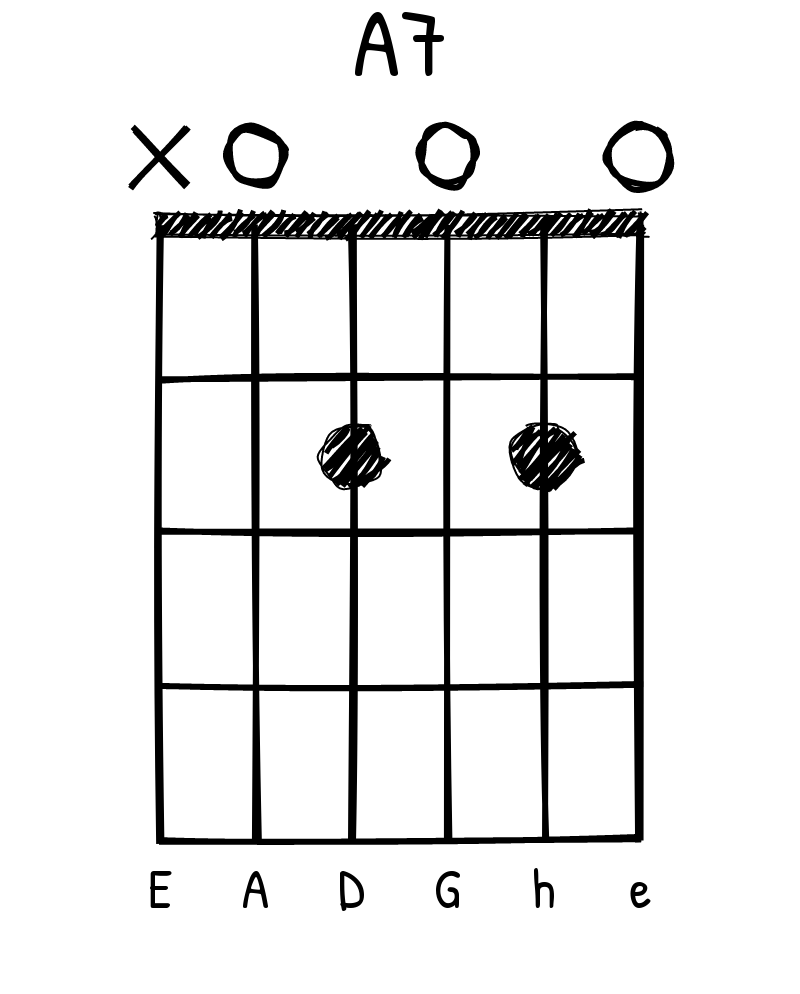
\includegraphics[height=3.5cm]{images/A7.png}
    \end{center}
    \vfill\null\columnbreak{}
    \begin{verse}
        W ciszy, czy w czasie burzy \\
        Trzeba przy pracy śpiewać \\
        Bo kiedy śpiewu nie ma \\
        Bo kiedy śpiewu nie ma \\
        Neptun się będzie gniewać
    \end{verse}
    \begin{verse}
        Neptun się będzie gniewać \\
        I klątwę brzydką rzuci \\
        Wpakuje na mieliznę \\
        Wpakuje na mieliznę \\
        Albo nam łódź wywróci
    \end{verse}
    \begin{verse}
        Albo nam łódź wywróci \\
        I krzyknie: \say{Hej, partacze! \\
        Nakarmię wami rybki \\
        Nakarmię wami rybki \\
        Nikt po was nie zapłacze!}
    \end{verse}
    \begin{verse}
        Nikt po nas nie zapłacze \\
        Nikt nam nie dopomoże \\
        Za wszystkie miłe rady \\
        Za wszystkie miłe rady \\
        Dziękuję tobie, Morze
    \end{verse}
    \begin{verse}
        Hej, Morze, moje Morze \\
        Wdzięczny ci jestem bardzo \\
        Toś ty mnie wychowało \\
        Toś ty mnie wychowało \\
        Szkołęś mi dało twardą
    \end{verse}
    \end{multicols}
\end{song}


\newpage
\begin{song}{title={Nazywali go Marynarz (Szanta narciarska)}, music={Artur Andrus}}
	\begin{intro}
	\writechord{d}
	\end{intro}    
    \begin{multicols}{2}
    \begin{verse}
        Nazy^{d}wali ^{C}go ma^{d}rynarz \\
        Bo o^{d}paskę ^{C}miał na ^{d}oku \\
        ^{g}Na każdym stoku dziew^{d}czyna \\
        Dziew^{B}czyna na ^{A}każdym s^{d}toku
    \end{verse}
    \begin{verse*}
        Po^{d}chodzi s^{C}pod Poz^{d}nania \\
        Po^{d}dobno ^{C}umie w^{F}różyć z kart \\
        ^{g}Panny rwie na wią^{d}zania \\
        Mę^{B}żatki --- ^{A}na długość ^{d}nart
    \end{verse*}
  	\begin{chorus}
        Ca^{d}ryco ^{A}mokrego ś^{d}niegu \\
        Ra^{d}trakiem płynę do ciebie pod ^{g}prąd --- hej! \\
        ^{g}Dobrze, że stoisz na ^{d}brzegu \\
        Bo ja ^{B}właśnie ^{A}schodzę na ^{d}ląd
    \end{chorus}
        \vfill\null\columnbreak{}
    \begin{verse}
        Nigdy się nie lękał biedy \\
        I się nie przejmował jutrem \\
        A jego ratrak był kiedyś \\
        Zwyczajnym, rybackim kutrem
    \end{verse}
    \begin{verse*}
        I woził dorsze i śledzie \\
        Zimą i latem, okrągły rok \\
        Teraz, jak nieraz przejedzie \\
        Rybami --- czuć cały stok
    \end{verse*}
    \begin{chorus}
        Caryco mokrego śniegu\ldots
    \end{chorus}
    \begin{verse}
        Wszyscy w porcie odetchnęli \\
        Zwiał, nim się zakończył sezon \\
        Jeszcze się tam, jak żagiel bieli \\
        Jego czarny kombinezon
    \end{verse}
    \begin{verse*}
        Odpłynął pod Ustrzyki \\
        I przez kobiety wpadł w kłopoty \\
        Forsę z polowań na orczyki \\
        Przehulał --- na antybiotyk
    \end{verse*}
    \begin{chorus}
        Caryco mokrego śniegu\ldots
    \end{chorus}
    \begin{verse}
        Jeśli kiedyś go zobaczysz \\
        Na ratraku w podłym świecie \\
        To powiedz mu, że w Karpaczu \\
        Czekają na niego dzieci
    \end{verse}
    \begin{verse*}
        I kiedy opuszcza statek \\
        Żeby się znowu oddać złu \\
        Każda z dwudziestu siedmiu matek \\
        Dzieciątku --- śpiewa do snu
    \end{verse*}
    \begin{chorus}
        Caryco mokrego śniegu\ldots $\times 2$
    \end{chorus}
    \end{multicols}
\end{song}


\newpage
\begin{song}{title={Pacyfik}, music={Mechanicy Shanty}}
    \begin{info}
        \textit{(zaczynamy od pierwszego wersu zwrotki i dodajemy kolejny za każdym razem)}
    \end{info}
    \begin{multicols}{2}
    \begin{verse*}
        ^{D}Kiedy szliśmy przez Pacyfik \\
        \textit{^{D}Way-hey! ^{A}Roluj go!}
    \end{verse*}
    \begin{verse}
        ^{D}Zwiało nam z pokładu skrzynki
    \end{verse}
    \begin{verse}
        Pełne śledzia i sardynki
    \end{verse}
    \begin{verse}
        Kosze krabów, beczkę sera
    \end{verse}
    \begin{verse}
        Kalesony oficera 
    \end{verse}
    \begin{verse}
        Sieć jeżowców, jedną żabę 
    \end{verse}
    \begin{verse}
        Kapitańską zmyło babę 
    \end{verse}
    \begin{verse}
        Beczki rumu nam nie zwiało 
    \end{verse}
    \begin{verse}
        Pół załogi ją trzymało
    \end{verse}
    \vfill\null\columnbreak{}
    \begin{verse*}
        \textit{^{D}Taki był cho^{A}lerny sz^*{D}torm !}
    \end{verse*}
    \begin{chorus}
        ^{D}Hej, znowu z^{G}myło coś \\
        ^{D}Zniknął w morzu ^{A}jakiś gość \\
        ^{D}Hej, policz k^{G}tóry tam \\
        ^{A}Jaki znowu zmyło ^{D}kram
    \end{chorus}
    \begin{outro}
        Hej, znowu zmyło coś \\
        Zniknął w morzu jakiś gość \\
        Postawcie wina dzban \\
        Opowiemy dalej wam!
    \end{outro}
    \end{multicols}
\end{song}


\newpage
\begin{song}{title={Pieśń wielorybników}, interpret={EKT Gdynia}, music={tradycyjna (Bonnie Ship the Diamond)}}
\begin{multicols}{2}
    \begin{intro}
        a a a d \\
        a e a a $\times 2$
    \end{intro}
    \begin{verse}
        Nasz D^{a}iament prawie g^{e}otów już \\
        W cieśn^{a}inach nie ma kr^{e}y \\
        Na k^{a}ei piękne pa^{e}nny stoją \\
        W ich o^{d}czach bły^{e}szczą ł^{a}zy \\
        Kapitan w niebo wlepia wzrok \\
        Ruszamy lada dzień \\
        Płyniemy tam, gdzie słońca blask \\
        nie mąci nocy cień
    \end{verse}
    \begin{chorus}
        A więc krz^{a}ycz: ^{e}o h^{a}o! \\
        Odw^{a}agę w s^{e}ercu mi^{a}ej \\
        Wielor^{a}ybów ci^{e}elska gr^{C}oźne s^{G}ą \\
        Lecz do^*{F}sta ni^{e}emy j^{a}e $\times 2$
    \end{chorus}
    \begin{chorus*}
        a a a d \\
        a e a a $\times 2$
    \end{chorus*}
    \begin{verse}
        Ej panno powiedz po co łzy \\
        Nic nie zatrzyma mnie \\
        Bo prędzej w wodach kwiat zakwitnie \\
        Niż wycofam się \\
        No nie płacz mała, wrócę tu \\
        Nasz los nie taki zły \\
        Bo da dukatów wór za tran \\
        I wielorybie kły
    \end{verse}
    \begin{chorus}
        A więc krzycz: o ho!\ldots $\times 2$
    \end{chorus}
    \begin{verse}
        Na deku stary wąchał wiatr \\
        lunetę w ręku miał \\
        Na łodziach co zwisały już \\
        z harpunem każdy stał \\
        I dmucha tu i dmucha tam  \\
        ogromne stado w krąg \\
        Harpuny, wiosła, liny brać \\
        I ciągnij brachu ciąg
    \end{verse}
    \begin{chorus}
        A więc krzycz: o ho!\ldots $\times 2$
    \end{chorus}
    \begin{verse}
        \textit{wolniej} \\
        I dla ^*{a}wielo ry^{G}ba j^{a}uż \\
        Os^*{e}ta tn^{G}i to dzi^{a}eń \\
        Bo śmi^{a}ały harp^*{C}u nn^{G}ik \\
        ^*{F}U de^{G}rza w^{a}eń
    \end{verse}
    \begin{outro}
        a a a d \\
        a e a a
    \end{outro}
\end{multicols}
\end{song}
\fancyfoot[LO,RE]{
\includegraphics[height=45pt]{images/docker.png}}

\newpage\pagestyle{szanty}
\newpage
\begin{song}{title={Pij za starego (Whiskey in the jar)}, music={Thin Lizzy}, interpret={Poszedłem Na Dziób}}
    \begin{intro}
        \writechord{F} \writechord{C} \writechord{G} \writechord{C}
    \end{intro}
    \begin{multicols}{2}
    \begin{verse}
        Pły^{C}nąłem w dół Cork City \\
        By ^{a}przejść przez Góry Kerry \\
        Spot^{F}kałem tam Farrella \\
        Co ^{C}forsę swoją liczył \\
        Sięg^{C}nąłem więc po spluwę \\
        A ^{a}potem po swój rapier \\
        Krzyk^{F}nąłem: \say{Dawaj forsę \\
        Jeśli ^{C}ci miłe życie!}
    \end{verse}
    \begin{chorus}
        $\times 2$ \\
        Masza ^{G}ring dama du dama da \\
        ^{C} Pij za starego \\
        ^{F} Pij za starego \\
        Bo ^{C}whiskey ^{G}pełny ^{C}słój
    \end{chorus}
    \begin{interlude}
        \writechord{F} \writechord{C} \writechord{G} \writechord{C}
    \end{interlude}
    \vfill\null\columnbreak{}
    \begin{verse}
        Zabrałem całą forsę \\
        A trochę tego było \\
        Zaniosłem worek szmalu \\
        Do domu pięknej Molly \\
        A ona przysięgała \\
        Że tylko o mnie śniła \\
        Lecz wnet się okazało \\
        Że tylko szmal mój woli
    \end{verse}
    \begin{chorus}
        Masza ring dama du dama da\ldots
    \end{chorus}
    \begin{interlude}
        \writechord{F} \writechord{C} \writechord{G} \writechord{C}
    \end{interlude}
    \begin{verse}
        Pijany i zmęczony \\
        Poszedłem znów do Molly \\
        Zabrałem jej szmal cały \\
        Nie wiedząc, co mnie czeka \\
        Lecz nagle tuż przede mną \\
        Kapitan Farrell stoi \\
        Strzeliłem więc z mej spluwy \\
        Trafiając w tego człeka
    \end{verse}
    \begin{chorus}
        Masza ring dama du dama da\ldots
    \end{chorus}
    \begin{interlude}
        \writechord{F} \writechord{C} \writechord{G} \writechord{C}
    \end{interlude}
    \begin{verse}
        Rybacy łowią ryby \\
        Myśliwi tną zwierzynę \\
        A ja lubię posłuchać \\
        Odgłosu kanonady \\
        I lubię mieć przy sobie \\
        Mą Molly, cud-dziewczynę \\
        Lecz teraz siedzę w celi \\
        I mam łańcuchów ślady
    \end{verse}
    \begin{chorus}
        Masza ring dama du dama da\ldots
    \end{chorus}
    \begin{interlude}
        \writechord{F} \writechord{C} \writechord{G} \writechord{C}
    \end{interlude}
    \end{multicols}
\end{song}


\newpage
\begin{song}{title={Pożegnanie Liverpoolu}, music={Cztery Refy}}
    \begin{verse}
        Żegnaj ^{C}nam, dos^{C7}tojny stary ^{F} por^{C}cie \\
        Rzeko ^{C}Mersey\footnotemark{}, ^{C}żegnaj ^{G}nam ^{G} \\
        Zaciąg^{C}nąłem się na ^{C7}rejs do Kali^*{F}for ^{C}nii \\
        Byłem ^{C}tam już nie ^{G}jeden ^{C}raz ^{C}
    \end{verse}
    \begin{chorus}
        A więc ^{G} żegnaj ^{G}mi, ko^{F}chana ^{C}ma \\
        Już za ^{C}chwilę wypły^{C}niemy w długi ^{G}rejs ^{G} \\
        Ile mie^{C}sięcy cię nie ^{C7}będę widział, ^{F} nie wiem ^{C}sam \\
        Lecz pa^{C}miętać zawsze ^{G}będę ^{C}cię ^{C}
    \end{chorus}
    \begin{verse}
        Zaciągnąłem się na herbaciany kliper \\
        Dobry statek, choć sławę ma złą \\
        A, że kapitanem jest tam stary Burgess\footnotemark{} \\
        Pływającym piekłem wszyscy go zwą
    \end{verse}
    \begin{chorus}
        A więc żegnaj mi, kochana ma\ldots
    \end{chorus}
    \begin{verse}
        Z tym kapitanem płynę już nie pierwszy raz \\
        Znamy się od wielu, wielu lat \\
        Jeśliś dobrym żeglarzem, radę sobie dasz \\
        Jeśli nie, toś cholernie wpadł
    \end{verse}
    \begin{chorus}
        A więc żegnaj mi, kochana ma\ldots
    \end{chorus}
    \begin{verse}
        Żegnaj nam, dostojny stary porcie \\
        Rzeko Mersey, żegnaj nam \\
        Wypływamy już na rejs do Kalifornii \\
        Gdy wrócimy, opowiemy wam
    \end{verse}
    \begin{chorus}
        A więc żegnaj mi, kochana ma\ldots
    \end{chorus}
    \footnotetext{wym.\ mersi}
    \footnotetext{wym.\ bardżes}
\end{song}


\newpage
\begin{song}{title={Press gang (Branka)}, music={Cztery refy}}
\begin{multicols}{2}
    \begin{verse}
        W dół od rzeki, poprzez London Street \\
        Psów królewskich oddział zwarty szedł \\
        Ojczyźnie trzeba dziś świeżej krwi \\
        Marynarzy floty wojennej
    \end{verse}
    \begin{verse}
        A że byłem wtedy silny chłop\\
        W tłumie złowił mnie sierżanta wzrok \\
        W kajdanach z bramy wywlekli mnie \\
        Marynarza floty wojennej
    \end{verse}
    \begin{verse}
        Jak o prawa upominać się \\
        Na gretingu nauczyli mnie \\
        Niejeden krwią wtedy spłynął grzbiet \\
        Marynarza floty wojennej
    \end{verse}
    \begin{verse}
        Nikt nie zliczy ile krwi i łez \\
        Wsiąkło w pokład, gdy się zaczął rejs \\
        Dla chwały twej, słodki kraju mój \\
        Marynarzy floty wojennej
    \end{verse}
    \begin{verse}
        Hen, za rufą miły został dom \\
        Jesteś tylko parą silnych rąk \\
        Dowódca tu twoim bogiem jest \\
        Marynarzu floty wojennej
    \end{verse}
    \begin{verse}
        Gdy łapaczy szyk formuje się \\
        W pierwszym rzędzie możesz ujrzeć mnie \\
        Kto stanie na mojej drodze dziś \\
        \textbf{Łup} stanowi floty wojennej
    \end{verse}
\end{multicols}
    \includegraphics[width=\textwidth]{sheet\string_music/cztery\string_refy-press\string_gang.png}
\end{song}

\newpage
\begin{song}{title={Przechyły}, interpret={Roman Roczeń}, music={Paweł Orkisz}}
    \begin{verse}
        Pierwszy ^{a}raz, przy ^{h}pełnym takie^{e}lunku \\
        Biorę s^{a}ter i ^{h}trzymam kurs na ^{e}wiatr \\
        I jest ^{a}jak przy ^{h}pierwszym poca^{e}łunku \\
        W ustach ^{C}sól, go^{H7}rącej wody ^{e}smak
    \end{verse}
    \begin{chorus}
        O ho ^{a}ho, prze^{h}chyły i prze^{e}chyły \\
        O ho ^{a}ho, za ^{h}falą fala m^{e}knie \\
        O ho ^{a}ho, trzy^{h}majcie się dziew^{e}czyny (za liny!) \\
        Ale ^{C}wiatr, ó^{H7}semka chyba ^{e}dmie $\times 2$
    \end{chorus}
    \begin{verse}
        Zwrot przez sztag? Okej, zaraz zrobię \\
        Słyszę, jak kapitan cicho klnie \\
        Gubię wiatr i zamiast w niego dziobem \\
        To on mnie --- od tyłu, kumple w śmiech
    \end{verse}
    \begin{chorus}
        O ho ho, przechyły i przechyły\ldots
    \end{chorus}
    \begin{verse}
        Ej, ty tam, za burtę wychylony \\
        Tu naprawdę się nie ma z czego śmiać \\
        Cicho siedź i lepiej proś Neptuna \\
        Żeby coś nie spadło ci na kark
    \end{verse}
    \begin{chorus}
        O ho ho, przechyły i przechyły\ldots
    \end{chorus}
    \begin{verse}
        Krople mgły, w deszczowych kropel pyle \\
        Tańczy jacht, po deskach spływa dzień \\
        Jutro znów wypłynę, bo odkryłem \\
        Że wciąż brzmi żeglarska, stara pieśń
    \end{verse}
    \begin{chorus}
        O ho ho, przechyły i przechyły\ldots
    \end{chorus}
\end{song}


\newpage
\begin{song}{title={Samantha}, music={Zejman \& Garkumpel}}
    \begin{multicols}{2}
    \begin{verse}
        ^{a} Ty nie jesteś ^{G}kliprem ^{a}sławnym \\
        ^{a} ``Cutty Sark'', czy ``^{G}Betty Lo^{a}u'' \\
        ^{F} W Pacyfiku ^{G}portach gw^{a}arnych \\
        ^{F} Nie zahuczy ^{G} w głowie ^{a}rum ^{G}
    \end{verse}
    \begin{verse}
        Nie dla ciebie są cyklony \\
        Hornu także nie opłyniesz \\
        W rejsie sławnym i szalonym \\
        W szancie starej nie zaginiesz
    \end{verse}
    \begin{chorus}
        Hej ``Sa^{F}mantha'', ech ``Samantha'' \\
        Kiedy wia^{C}tr ci gra na w^{a}antach \\
        Gdy ry^{F}sujesz wody t^{d}aflę \\
        Moje ^{a}serce masz pod gaflem \\
        Czasem ^{C}ciężko prujesz wodę \\
        I twe ^{a}żagle już nienowe \\
        Jesteś ^{F}łajbą pełną wz^{G}ruszeń \\
        Jesteś ^{a}łajbą, ^{G} co ma ^{a}duszę ^{G}
    \end{chorus}
    \vfill\null\columnbreak{}
    \begin{verse}
        Ale teraz wyznać pora \\
        Chociaż nie wiem czemu, psiakość \\
        Gdy cię nie ma na jeziorach \\
        Na jeziorach pusto jakoś
    \end{verse}
    \begin{verse}
        Gdy w wieczornej przyjdzie porze \\
        Śpiewać zwrotki piosnki złudnej \\
        Gdy cię nie ma na jeziorze \\
        To Mazury nie są cudne
    \end{verse}
    \begin{chorus}
        Hej ``Samantha'', ech ``Samantha''\ldots
    \end{chorus}
    \begin{verse}
        Czasem, kiedyś już zmęczona \\
        W chwili krótkiej przyjemności \\
        W złotych słońca stu ramionach \\
        Ty wygrzewasz stare kości
    \end{verse}
    \begin{verse}
        A gdy przyjdzie kres twych dróg \\
        Nie zapłaczę na pogrzebie \\
        Wiem, że sprawi dobry Bóg \\
        Byś pływała dalej w niebie, hej!
    \end{verse}
    \begin{chorus}
        Hej ``Samantha'', ech ``Samantha''\ldots $\times 2$
    \end{chorus}
    \end{multicols}
\end{song}


\newpage
\newcommand{\tqs}{\textquotesingle}
\begin{song}{title={Santiano}, interpret={Hugues Aufray}, music={tradycyjna}, capo=2}
    \begin{verse}
        C\tqs est ^{e}un fameux trois-mâts, fin comme un oise^{D}au \\
        Hissez ^{e}haut ! « Santi^{D}ano » ! \\
        ^{a}Dix-huit nœuds, quatre ^{D}cents tonne^{h}aux \\
        Je suis ^{e}fier d\tqs y ^{h}être ^{e}matelot
    \end{verse}
    \begin{chorus}
        Tiens ^{e}bon la vague et tiens bon le ^{D}vent \\
        Hissez ^{e}haut ! « Santi^{D}ano » ! \\
        ^{a}Si Dieu veut, toujours ^{D}droit de^{h}vant \\
        Nous i^{e}rons jus^{h}qu\tqs à San ^{e}Francisco
    \end{chorus}
    \begin{verse}
        Je pars pour de longs mois en laissant Margot \\
        Hissez haut ! « Santiano » ! \\
        D\tqs y penser, j\tqs avais le cœur gros \\
        En doublant les feux de Saint-Malo
    \end{verse}
    \begin{chorus}
        Tiens bon la vague et tiens bon le vent\ldots
    \end{chorus}
    \begin{verse}
        On prétend que là-bas, l\tqs argent coule à flots \\
        Hissez haut ! « Santiano » ! \\
        On trouve l\tqs or au fond des ruisseaux \\
        J'en ramènerai plusieurs lingots
    \end{verse}
    \begin{chorus}
        Tiens bon la vague et tiens bon le vent\ldots
    \end{chorus}
    \begin{verse}
        Un jour je reviendrai, chargé de cadeaux \\
        Hissez haut ! « Santiano » ! \\
        Au pays, j\tqs irai voir Margot \\
        À son doigt, je passerai l\tqs anneau
    \end{verse}
    \begin{chorus}
        Tiens bon le cap et tiens bon le flot \\
        Hissez haut ! « Santiano » ! \\
        Sur la mer qui fait le gros dos \\
        Nous irons jusqu\tqs à San Francisco $\times 2$
    \end{chorus}
\end{song}


\newpage
\begin{song}{title={Stara Maui}, music={Mechanicy Shanty}}
    \begin{multicols}{2}
    \begin{verse}
        Mo^{d}zolny, ^{A}twardy i ^{d}trudny ^{C}jest \\
        Nasz wie^*{d}loryb ^{A}niczy z^{d}nój \\
        Lecz ^{d}nie przest^{A}raszy nas sz^{d}tormów ^{C}ryk \\
        I nie z^{d}lęknie ^{A}groza ^{d}burz \smallskip \\
        Dziś pow^{F}rotnym kursem wra^{C}camy już ^{A} \\
        Rejsu ^{d}chyba to ostatnie ^{A}dni \\
        I ^{d}każdy w ^{A}sercu już ^{d}chyba ^{C}ma \\
        Piękne ^{B}panny ^{A}ze Starej Ma^{d}ui
    \end{verse}
    \begin{chorus}
        Płyńmy w ^{F}dół, do Starej Ma^{C}ui (już ^{A}czas!) \\
        Płyńmy w ^{d}dół, do Starej Ma^{A}ui \\
        Ark^{d}tyki b^{A}lask już po^{d}żegnać ^{C}czas \\
        Płyńmy w ^{B}dół, do ^{A}Starej Ma^{d}ui
    \end{chorus}
    \vfill\null\columnbreak{}
    \begin{verse}
        Z północnym sztormem już płynąć czas \\
        Wśród lodowych, groźnych gór \\
        I dobrze wiemy, że nadszedł czas \\
        Ujrzeć niebo z tropikalnych chmur \smallskip \\
        Dziesięć długich miesięcy zostało gdzieś \\
        Wśród piekielnej, kamczackiej mgły \\
        Żegnamy już Arktyki blask \\
        I płyniemy do Starej Maui
    \end{verse}
    \begin{chorus}
        Płyńmy w dół, do Starej Maui (już czas!)\ldots
    \end{chorus}
    \begin{verse}
        Harpuny już odłożyć czas \\
        Starczy, dość już wielorybiej krwi \\
        Już pełne tranu beczki masz \\
        Płynne złoto sprzedasz w mig \smallskip\\
        Za swój żywot psi, za trud i znój \\
        Kiedyś w niebie dostaniesz złoty tron \\
        O dzięki Ci, Boże, że każdy mógł \\
        Wrócić do rodzinnych stron
    \end{verse}
    \begin{chorus}
        Płyńmy w dół, do Starej Maui (już czas!)\ldots
    \end{chorus}
    \begin{verse}
        Kotwica mocno już trzyma dno \\
        Wreszcie ujrzysz ukochany dom \\
        Przed nami główki portu już \\
        I kościelny słychać dzwon \smallskip \\
        A na lądzie uciech nas czeka sto \\
        Wnet zobaczysz dziatki swe \\
        Na spacer weźmiesz żonę swą \\
        I zapomnisz wszystkie chwile złe
    \end{verse}
    \begin{chorus}
        Płyńmy w dół, do Starej Maui (już czas!)\ldots $\times 2$
    \end{chorus}
    \end{multicols}
\end{song}


\newpage
\begin{song}{title={Stary bryg}, music={EKT Gdynia}}
    \begin{intro}
        \writechord{d} \writechord{a} \writechord{d} \writechord{G} $\times 2$
    \end{intro}
    \begin{verse}
        ^{d} Gdy wy^{a}pływał z ^{d}portu ^{a}stary bryg ^{d} ^{a} ^{d} ^{G} \\
        ^{d}Jego ^{C}dalszych ^{F}losów ^{C}nie znał ^{d}nikt ^{a} ^{d} ^{G} \\
        ^{d}Nikt nie wiedział ^{F}o tym, że \\
        ^{G}Statkiem-widmem ^{a}stanie się stary ^{d}bryg ^{a} ^{d} ^{G} \\
        ^{d} ^{a} ^{d} ^{G}
    \end{verse}
    \begin{chorus}
        ^{d}Hej, ^{F}ho! ^{C}na umrzyka ^{d}skrzyni \\
        ^{F}I bu^{C}telka ^{d}rumu ^{a} ^{d} ^{G} \\
        ^{d}Hej, ^{F}ho! ^{C}resztę czas u^{d}czyni \\
        ^{F}I bu^{C}telka ^{d}rumu ^{a} ^{d} ^{G} \\
        ^{d} ^{a} ^{d} ^{G}
    \end{chorus}
    \begin{verse}
        Co z załogą zrobił stary bryg \\
        Tego też nie zgadnie chyba nikt \\
        Czy zostawił w porcie ją \\
        Czy na morza dnie? Nikt nie wie gdzie
    \end{verse}
    \begin{chorus}
        Hej, ho! na umrzyka skrzyni\ldots
    \end{chorus}
    \begin{verse}
        Przepowiednia zła jest, że ho ho \\
        Kto go spotka, marny jego los \\
        Ale my nie martwmy się \\
        Hej, nie martwmy się --- rum jeszcze jest!
    \end{verse}
    \begin{chorus}
        Hej, ho! na umrzyka skrzyni\ldots $\times 2$ 
    \end{chorus}
\end{song}


\newpage
\begin{song}{title={Stary wrak}, music={Mechanicy Shanty}}
\small
    \begin{intro}
        \writechord{d} \writechord{a} \\
        \writechord{C} \writechord{D}\writechord{G} \\
        \writechord{a} \writechord{G} \writechord{asus2}
    \end{intro}
    \begin{multicols}{2}
    \begin{verse}
        Już za^{d}kończył życie swe ^{a} \\
        Oparł ^{C}dziób o stro^{D}my ^{G}brzeg \\
        Rejsu ^{a}kres wyznaczył cz^{G}as i morza gniew ^{asus2} \\
        Już pozostał tylko ślad \\
        Żagli, które targał wiatr \\
        Nie zawiodą go już więcej na swój szlak
    \end{verse}
    \begin{chorus*}
        Tam gdzieś ^{a}czeka na nas znów \\
        Żagli ^{G}biel i silny wiatr \\
        Tam gdzieś ^{a}czeka żywioł, który wciąż nas ^{F}gna \\
        Gdzieś do ^{d}postrzępionych pa^{a}lm \\
        Do mil^{C}czących, zło^{D}tych ^{G}plaż \\
        Stary ^{a}wrak na pokład j^{G}uż nie weźmie nas ^{asus2}
    \end{chorus*}
    \begin{center}
        \vspace{0.6cm}
        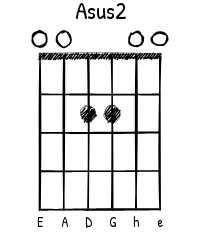
\includegraphics[height=3.5cm]{images/Asus2.png}
    \end{center}
    \vfill\null\columnbreak{}
    \begin{verse}
        Dzielny był przez tyle lat \\
        ``Czarnej Kuli'' nosił znak \\
        Imię jego wśród liniowców każdy znał \\
        Gdy na cumach w porcie stał \\
        Smukłe linie, piękny kształt \\
        Każdy morze razem z nim zdobywać chciał
    \end{verse}
    \begin{chorus*}
        Płynąć tam, gdzie czeka znów \\
        Żagli biel i silny wiatr \\
        Płynąć tam, gdzie żywioł, który wciąż nas gna \\
        Gdzieś do postrzępionych palm \\
        Do milczących, złotych plaż \\
        Dziś na pokład stary wrak nie weźmie nas
    \end{chorus*}
    \begin{verse}
        To wędrówki jego kres \\
        Skończył się już żagli wiek \\
        Nie powrócą pod błękitny nieba dach \\
        Tylko w sercach naszych trwa \\
        Do żaglowców z tamtych lat \\
        Wielka miłość, która w morze ciągnie nas
    \end{verse}
    \begin{chorus*}
        Chcemy płynąć tam, gdzie znów \\
        Żagli biel i silny wiatr \\
        Chcemy płynąć w żywioł, który wciąż nas gna \\
        Tam do postrzępionych palm \\
        Do milczących, złotych plaż \\
        Stary wrak wciąż pływać będzie w naszych snach
    \end{chorus*}
    \begin{interlude}
        Tam do postrzępionych palm \\
        Do milczących, złotych plaż \\
        Stary wrak wciąż pływać będzie w naszych snach
    \end{interlude}
    \end{multicols}
\end{song}


\newpage
\fancyfoot[LO,RE]{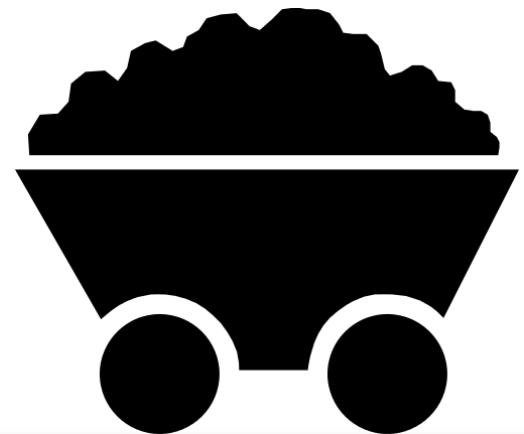
\includegraphics[height=45pt]{images/miner_cart.png}}
\begin{song}{title={Szesnaście ton}, music={Merle Travis}, lyrics={Marek Szurawski}}
    \begin{intro}
        \writechord{e}
    \end{intro}
    \begin{verse}
        Ktoś ^{e}mówił, że z gliny u^{e}lepił mnie Pan  \\
        A ^{e}przecież się składam z ^{e}kości i krwi  \\
        Z ^{e}kości i krwi, ^{a}jarzma na kark \\
        I ^{H7}pary rąk, pary ^{e}silnych rąk
    \end{verse}
    \begin{chorus}
        Co dzień szes^{e}naście ton, i ^{e}co z tego mam \\
        Tym ^{e}więcej mam długów, im ^{e}więcej mam lat \\
        Nie ^{e}wołaj Święty Piotrze, j^{a}a nie mogę przyjść \\
        Bo ^{H7}duszę swoją od^{C7}dałem za ^{e}dług\footnotemark{}
    \end{chorus}
    \begin{verse}
        Gdy matka mnie rodziła, pochmurny był dzień \\
        Więc wziąłem szuflę, poszedłem pod szyb \\
        Nadzorca mi rzekł: \say{Nie zbawi cię Pan  \\
        Załaduj co dzień szesnaście ton}
    \end{verse}
    \begin{chorus}
        Co dzień szesnaście ton\ldots
    \end{chorus}
    \begin{verse}
        Czort może dałby radę, a może i nie \\
        Szesnastu tonom podołać co dzień \\ 
        Szesnaście ton, szesnaście jak drut \\
        Codziennie nie da rady nawet dwóch
    \end{verse}
    \begin{chorus}
        Co dzień szesnaście ton\ldots
    \end{chorus}
    \begin{verse}
        Gdy kiedyś spotkasz mnie, lepiej z drogi mi zejdź \\
        Bo byli już tacy --- nie pytaj, gdzie są  \\
        Nie pytaj, gdzie są, bo zawsze jest ktoś \\
        Nie ten, to ów, co urządzi cię
    \end{verse}
    \begin{chorus}
        Co dzień szesnaście ton\ldots
    \end{chorus}
    \footnotetext{monopol w miasteczkach górniczych w USA powodował, że koszty życia przewyższały zarobki}
\end{song}

\newpage\pagestyle{szanty}
\newpage
\begin{song}{title={Szkuner „I'm Alone“}, music={Smugglers}}
    \small
    \begin{intro}
        \writechord{C} \writechord{a} \writechord{e}
    \end{intro}
    \begin{verse}
        Baksz^{e}tagiem pruł nasz \say{I'm Alone} hen, ^{G}od Meksyku b^{D}ram \\
        A ^{a}jankes, w dziób kopany, po ^{e}piętach deptał nam \\
        Ty^{e}siące beczek ^{G}rumu, od lo^{D}kerów aż po dno \\
        I ^{a}nawet kabla luzu, choćbyś r^{e}obił nie wiem co
    \end{verse}
    \begin{chorus}
        Sam ^{C}Neptun śpiewał szanty, po ^{G}cichu sprzyjał nam \\
        Więc ^{a}bił rekordy \say{I'm Alone}, choć g^{H7}roził wciąż Wuj Sam \\
        Na ^{C}jedną kartę wszystko, jak s^{G}truna k^{H}ażdy ^{e}bras \\
        \say{Niech di^{a}abli porwą Coast Guard} --- tak ^{e}mawiał każdy z nas
    \end{chorus}
    \begin{verse}
        A dawniej szkuner \say{I'm Alone} hen, po łowiskach gnał \\
        Lecz w końcu ryb zabrakło i głód w oczy zajrzał nam \\
        Za burty poszły sieci, bo tak krzyczał kobiet tłum \\
        Jankesi mają ginu dość, postawmy więc na rum
    \end{verse}
    \begin{chorus}
        Sam Neptun śpiewał szanty, po cichu sprzyjał nam\ldots
    \end{chorus}
    \begin{verse}
        Gdy stawialiśmy żagle, to Coast Guard wpadał w trans \\
        Ta banda bubków w baliach nie miała żadnych szans \\
        Pułapki zastawili, gnoje, choć tak dobrze szło \\
        Posłali dzielny \say{I'm Alone} z ładunkiem aż na dno
    \end{verse}
    \begin{verse*}
        Niejeden z Nowej Szkocji szkuner taki spotkał los \\
        A wszystko przez cholerny głód i wiecznie pusty trzos \\
        Lecz jeden z nich, nasz \say{I'm Alone} swe miejsce w pieśni ma \\
        I pewnie Neptun lubi go i w kości na nim gra
    \end{verse*}
    \begin{chorus}
        I nawet śpiewa szanty, po cichu sprzyja nam \\
        Choć leży na dnie \say{I'm Alone} i śmieje się Wuj Sam \\
        Na jedną kartę wszystko, jak struna każdy bras \\
        \say{Niech diabli porwą Coast Guard} --- tak mawiał każdy z nas
    \end{chorus}
    \begin{verse}
        A ci, co pokład \say{I'm Alone} kochali, jak swój dom \\
        Nie dla nich blaski sławy i nie dla nich w niebie tron \\
        Niech mają choć ten cichy klang, ten jeden marny dzwon \\
        I niech każdy do nich woła: \say{Hej, smuggler z \say{I'm Alone!}}
    \end{verse}
    \begin{chorus}
        Niech Neptun śpiewa szanty, po cichu sprzyja nam \\
        Rekordy bije \say{I'm Alone} i zamknie się Wuj Sam \\
        Na jedną kartę wszystko, jak struna każdy bras \\
        \say{Niech smuggler pije tylko rum!} --- tak mawia każdy znas $\times 2$
    \end{chorus}
    \begin{outro}
        \writechord{C} \writechord{a} \writechord{e}
    \end{outro}
\end{song}


\newpage
\begin{song}{title={Wellerman}, music={tradycyjna}, capo=3}
\begin{multicols}{2}
    \begin{verse}
        There o^{a}nce was a ship that put to sea \\
        And the na^{d}me of that ship was the ^{a}Billy o' Tea \\
        The ^{a}winds blew hard, her bow dipped down \\
        ^{e}Blow, me bully boys, ^{a}blow (huh)
    \end{verse}
    \begin{chorus}
        ^{F}Soon may the ^{C}Wellerman come \\
        To ^{d}bring us sugar and ^{a}tea and rum \\
        ^{F}One day, when the ^{C}tonguing is done \\
        We'll ^{e}take our leave and ^{a}go
    \end{chorus}
    \begin{verse}
        She had not been two weeks from shore \\
        When down on her a right whale bore \\
        The captain called all hands and swore \\
        He'd take that whale in tow (huh) 
    \end{verse}
    \begin{chorus}
        Soon may the Wellerman come\ldots
    \end{chorus}
    \vfill\null\columnbreak{}
    \begin{verse}
        Before the boat had hit the water \\
        The whale's tail came up and caught her \\
        All hands to the side, harpooned and fought her \\
        When she dived down below (huh)
    \end{verse}
    \begin{chorus}
        Soon may the Wellerman come\ldots
    \end{chorus}
    \begin{verse}
        No line was cut, no whale was freed \\
        An' the captain's mind was not on greed \\
        But he belonged to the Whaleman's creed \\
        She took that ship in tow (huh)
    \end{verse}
    \begin{chorus}
        Soon may the Wellerman come\ldots
    \end{chorus}
    \begin{verse}
        For forty days or even more (ooh) \\
        The line went slack then tight once more \\
        All boats were lost, there were only four \\
        And still that whale did go
    \end{verse}
    \begin{chorus}
        Soon may the Wellerman come\ldots
    \end{chorus}
    \begin{verse}
        As far as I've heard, the fight's still on \\
        The line's not cut, and the whale's not gone \\
        The Wellerman makes his regular call \\
        To encourage the captain, crew and all
    \end{verse}
    \begin{chorus}
        Soon may the Wellerman come\ldots $\times 2$
    \end{chorus}
\end{multicols}
\end{song}

\newpage\pagestyle{szanty}

\chapter{Poezja śpiewana}
\begin{center}
    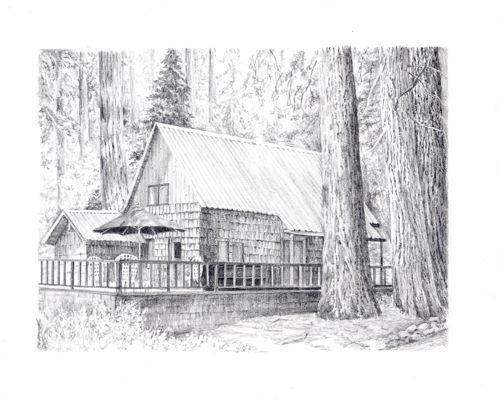
\includegraphics[width=0.5\textwidth]{images/chatka.jpg}
\end{center}
\pagestyle{poezja}
\newpage
\begin{song}{title={1788}, music={Jacek Kaczmarski}}
    \small
    \begin{intro}
        \writechord{F} \writechord{B} \writechord{F} \writechord{C} \\ 
        \writechord{F} \writechord{B} \writechord{F} \writechord{C} \writechord{F}
    \end{intro}
    \begin{multicols}{2}
\begin{verse}
^{F}Ta pierwsza morska ^{B}podróż do Australii! \\
^{F}Łotry przy burtach, prosty^{C}tutki w kojach \\
^{F}Wszyscy się bali, łk^{B}ali i rzygali \\
^{F}W drodze do raju. Przewrot^{C}ności Twoja \\
^{d}Panie, coś w jeszcze nam niezn^{g}anych planach \\
^{d} Miał czarne diabły strzeg^{a}ące wybrzeży \\
^{B}Edenu, który prz^{C}eznaczyłeś ^{F}dla nas \\
A w kt^{B}óry nikt, prawdę ^{C}mówiąc, nie ^{d}wierzył! \\
\\
^{d} ^{B} ^{F} ^{C}
\end{verse}
\begin{verse}
Czym żeśmy, marni, zasłużyli na to? \\
Ten, co zawisnąć miał za kradzież płaszcza \\
Płakał nad swoją niechybną zatratą \\
Nie widział Ciebie w robaczywych masztach \\
Statku, co tylko był więzieniem nowym \\
Tej co kupczyła ciałami swych dziatek \\ 
Ani przez mgnienie nie przyszło do głowy \\
Że to nadziei - nie rozpaczy statek \\
\end{verse}
\begin{verse}
Niejeden żołnierz z ponurej eskorty \\
Bo czym się ich los od naszego różnił? \\ 
Wiedział, że nigdy już nie ujrzy portu \\
Gdzie go podejmą karczmarze usłużni \\ 
I płatne dziewki; że zabraknie rumu \\
Zanim do celu przygnasz okręt szparki \\
Z marynarzami pili więc na umór \\
I - wbrew zakazom - grali o więźniarki \\
\end{verse}
\begin{verse}
Prawda, nie wszyscy próby Twe przetrwali \\
Ale też ciężkoś nas doświadczał, Panie \\
Nie oszczędzałeś nam wysokiej fali \\ 
Za którą mnogim przyszło w oceanie \\
Zakończyć żywot; innym dziąsła zgniły \\
Wypadły zęby, rozgorzały wrzody \\ 
Więc znaczą nasz zielony szlak mogiły \\
Szkorbutu, szału, francuskiej choroby \\
\end{verse}
\begin{verse}
Nikt nie odnajdzie w ruchomych otchłaniach \\
Ciał nieszczęśników - oprócz Ciebie, Boże \\
Ich żywot grzeszny epitafiów wzbrania \\
Lecz - ukarani. Więc wystarczy może \\ 
Żeś się posłużył straszliwym przykładem \\
Oni naprawdę dotarli do piekieł \\
A umierając nie wierzył z nich żaden \\
Że w swym cierpieniu umiera - człowiekiem \\
\end{verse}
\begin{verse}
Ląd nam się wydał niegościnny, dziki \\
Łotr bez honoru, kobieta sprzedajna \\
Z dnia na dzień - jak się stać ma osadnikiem \\
Nieznanych światów? Bo rozpoznać Raj nam \\
Nie było łatwo; znaleźć w sobie siłę \\
Wbrew przeciwnościom, bez słowa zachęty \\
By mimo wszystko żyć - nim nam odkryłeś \\ 
Kraj szczodry w zboże, złoto i diamenty \\
\end{verse}
\begin{verse}
^{d}Łajdacki pomiot, łot^{g}rowskie nasienie \\
^{d}Czerpiąc ze spichrza Twoich d^{a}óbr wszelakich \\
^{B}Choć tyle wiemy w^{C}łasnym doświadcz^{F}eniem \\
^{d}W nas jest Raj, Pi^{B}ekło - ^{F}I do obu-szl^{C}aki \\
^{d}W nas jest Raj, Pi^{B}ekło - ^{F}I do obu-szl^{C}aki \\
^{d}W nas jest Raj, Pi^{B}ekło - ^{F}I do obu-szl^{C}aki \\
\\
\writechord{d} \writechord{B} \writechord{F} \writechord{C}
\end{verse}
\end{multicols}
\begin{center}
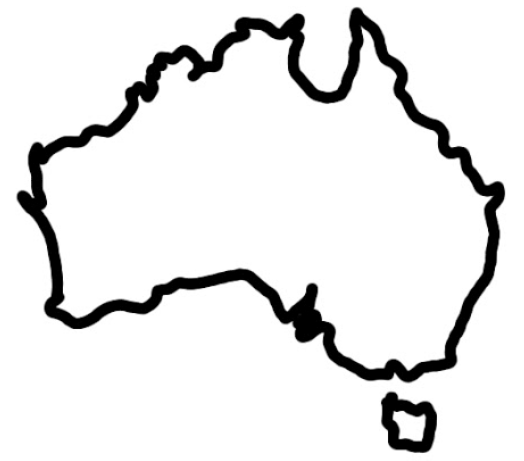
\includegraphics[width=0.15\textwidth]{images/1788.png}  
\end{center}
\end{song}
\newpage
\newpage\pagestyle{poezja}
\newpage
\begin{song}{title={Ballada na złe drogi}, music={EKT Gdynia}}
\begin{multicols}{2}
    \begin{intro}
        \writechord{a} \writechord{F} \writechord{d} \writechord{E} $\times 2$
    \end{intro}
    \begin{verse}
        ^{d} Na drogi złe, ^{E}dni zwyczajne \\
        ^{a} I na najwyższe ^{F} z progów \\
        ^{d} Dostaliśmy w ^{E}dłonie balladę \\
        ^{a} I pachnie jak ^{A}owoc głogu
    \end{verse}
    \begin{chorus}
        ^{d} I będzie prze^{G}biegać muzyka \\
        Czy ty ^{C}wiesz, jak to dużo po dniu ^{F} \\
        ^{d} I w wierszu nam ^{E}będzie rozkwitać \\
        Bal^{a}lada --- posag m^{A}ój \\
        ^{d} I będzie prze^{G}biegać muzyka \\
        Czy ty ^{C}wiesz, jak to dużo po dniu ^{F} \\
        ^{d} I w wierszu nam ^{E}będzie rozkwitać ballada 
    \end{chorus}
    \begin{interlude}
        \writechord{a} \writechord{F} \writechord{d} \writechord{E} $\times 2$
    \end{interlude}
    \vfill\null{}
    \columnbreak{}
    \begin{verse}
        Na ludzi o szarych obliczach \\
        Na ścieżki i wilcze doły \\
        Gdy zechcę, na głos będzie krzyczeć \\
        I w miejscu nam nie ustoi
    \end{verse}
    \begin{chorus}
        I będzie przebiegać muzyka\ldots
    \end{chorus}
    \begin{interlude}
        \writechord{a} \writechord{F} \writechord{d} \writechord{E} $\times 2$
    \end{interlude}
    \begin{verse}
        A kiedy będziemy odchodzić \\
        Hen, do Krainy Łowów \\
        Błękitne się niebo otworzy \\
        I spadnie jak owoc głogu
    \end{verse}
    \begin{chorus}
        I będzie przebiegać muzyka\ldots
    \end{chorus}
    \begin{interlude}
        \writechord{a} \writechord{F} \writechord{d} \writechord{E} $\times 2$
    \end{interlude}
\end{multicols}
\end{song}


\newpage
\begin{song}{title={Dni, których nie znamy}, music={Jan Kanty Pawluśkiewicz}, lyrics={Marek Grechuta}, capo=3}
%\begin{multicols}{2}
    \begin{intro}
   		\textit{akordy jak w zwrotce}
   	\end{intro}
   	\begin{verse}
   		^{a}Tyle było ^{C}dni d^{G}o utraty s^{C}ił \\
		^{d}Do utraty t^{A}chu t^{C}yle było chw^{G}il \\
		^{a}Gdy żałujesz t^{C}ych z któ^{G}rych nie masz ^{C}nic \\
		^{d}Jedno warto zn^{A}ać je^{C}dno tylko wie^{G}dz
   	\end{verse}
   	\begin{chorus}
   		Że w^{F}ażne są tyl^{d}ko te dni^{E7}, których jes^{a}zcze nie zn^*{F}a m^{G}y ^{C} \\
		Ważnych jest kilka tych chwil, tych, na które czekamy \\
		Ważne są tylko te dni, których jeszcze nie znamy \\
		Ważnych jest kilka tych chwil, tych, na które czekamy
   	\end{chorus}
   	\begin{verse}
   		Pewien znany ktoś kto miał dom i sad \\
		Zgubił nagle sens i w złe kręgi wpadł \\
		Choć majątek prysł on nie stoczył się \\
		Wytłumaczyć umiał sobie wtedy właśnie, że 
   	\end{verse}
   	\begin{chorus}
   		Ważne są tylko te dni, których jeszcze nie znamy \ldots
   	\end{chorus}
   	\begin{interlude}
   		^{a}Jak rozpoznać lu^{G}dzi ^{C}których już nie zn^{G}amy \\
	   	^{a}Jak pozbierać my^{G}śli ^{C}z tych nieposkład^{G}anych \\
	   	^{d}Jak oddzielić na^{A}gle ^{F}serce od ro^{C}zumu \\
   		^{a}Jak usłyszeć si^{G}ebie ^{C}pośród śpiewu tł^{G}umu \\
		Jak rozpoznać ludzi których już nie znamy \\
		Jak pozbierać myśli z tych nieposkładanych \\
		Jak odnaleźć nagle radość i nadzieje \\ 
		Odpowiedzi szukaj czasu jest tak wiele
   	\end{interlude}
   	\begin{chorus}
   		Ważne są tylko te dni, których jeszcze nie znamy \ldots
   	\end{chorus}
%\end{multicols}
\end{song}
\fancyfoot[LO,RE]{
\includegraphics[width=2cm]{images/piano.png}}

\newpage\pagestyle{poezja}
\newpage
\begin{song}{title={Jak}, lyrics={Edward Stachura}, music={Stare Dobre Małżeństwo}}
    \begin{intro}
        \writechord{C}
    \end{intro}
    \begin{verse*}
        ^{C}Jak po nocnym niebie su^{G}nące białe ob^{F}łoki nad l^{C}asem \\
        Jak na ^{d}szyi wędrowca apa^{F}szka szamotana wi^{C}atrem 
    \end{verse*}
    \begin{verse*}
        Jak wyciągnięte tam powyżej gwiaździste ramiona wasze \\
        A tu są nasze, a tu są nasze
    \end{verse*}
    \begin{verse*}
        Jak suchy szloch w tę dżdżystą noc \\
        Jak winny-li-niewinny sumienia wyrzut \\
        Że się żyje, gdy umarło tylu, tylu, tylu 
    \end{verse*}
    \begin{verse*}
        Jak suchy szloch w tę dżdżystą noc \\
        Jak lizać rany celnie zadane \\
        Jak lepić serce w proch potrzaskane
    \end{verse*}
    \begin{verse*}     
        Jak suchy szloch w tę dżdżystą noc \\
        Pudowy kamień, pudowy kamień \\
        Ja na nim stanę, on na mnie stanie \\
        On na mnie stanie, spod niego wstanę 
    \end{verse*}
    \begin{verse*}
        Jak suchy szloch w tę dżdżystą noc \\
        Jak złota kula nad wodami \\
        Jak świt pod spuchniętymi powiekami
    \end{verse*}
    \begin{verse*}
        Jak zorze miłe, śliczne polany \\
        Jak słońca pierś, jak garb swój nieść \\
        Jak do was, siostry mgławicowe, ten zawodzący śpiew
    \end{verse*}
    \begin{verse*}
        Jak biec do końca, potem odpoczniesz, potem odpoczniesz \\
        Cudne manowce, cudne manowce, cudne, cudne manowce $\times 2$
    \end{verse*}
    \begin{verse*}
        Na na na na na, na na na \\
        Na na na, na na na na \\
        Na na, na na na na \\
        Na na na na
    \end{verse*}
    \begin{verse*}
        Jak biec do końca, potem odpoczniesz, potem odpoczniesz \\
        Cudne manowce, cudne manowce, cudne, cudne manowce $\times 2$
    \end{verse*}
    \begin{verse*}
        \textit{wolniej} \\
        Jak biec do końca, potem odpoczniesz, potem odpoczniesz \\
        Cudne manowce, cudne manowce, cudne, cudne manowce
    \end{verse*}
\end{song}


\newpage
\begin{song}{title={Jaka jesteś}, music={Tomasz Lewandowski}}
	\begin{intro}
	\writechord{G} \writechord{a} \writechord{C} \writechord{D} $\times 2$
	\end{intro}    
    \begin{verse}
        Jesteś ^{G}bitwą moją ni^{a}eskończoną \\
        ^{C} W której ciągle ^{D} o przyczułek wa^{G}lczę ^{a} ^{C} ^{D} \\
        Jesteś ^{G}drzwiami, które o^{a}tworzyłem \\
        ^{C} A potem ^{D} przycięły mi p^{G}alce ^{a} ^{C} ^{D}
    \end{verse}
  	\begin{chorus}
        Jesteś ^{G}kartką z kalendarza ^{a} \\
        Zagub^{C}ioną gdzieś pomię^{D}dzy szuflad^{G}ami ^{a} ^{C} ^{D} \\
        I u^{G}licą, na któ^{a}rej co dzień \\
        ^{C} Uciekałem mi^{D}ędzy latar^{G}niami ^{a} ^{C} ^{D}
    \end{chorus}
    \begin{verse}
        Jesteś mgłą ogromną niezmierzoną \\
        Ciszą w huku i łoskotem w ciszy \\
        Jesteś piórem i wyblakłą kartką \\
        Którym i na której dzisiaj piszę
    \end{verse}
    \begin{chorus}
        Jesteś kartką z kalendarza\ldots
    \end{chorus}
    \begin{interlude}
        \writechord{G} \writechord{F} \writechord{C} \writechord{D} $\times 2$
    \end{interlude}
    \begin{verse}
        Przyszłaś do mnie, a ja nie spostrzegłem \\
        Dzisiaj tylko mogę mówić: \say{Byłaś\ldots} \\
        Nie wiem czy na jawie wzięłaś mnie za rękę \\
        Czy jak wszystko ty się tylko sniłaś
    \end{verse}
    \begin{chorus}
        Że jesteś kartką z kalendarza\ldots $\times 2$
    \end{chorus}
\end{song}


\newpage
\begin{song}{title={Jest już za późno}, lyrics={Edward Stachura}, music={Stare Dobre Małżeństwo}}
    \begin{intro}
        \writechord{C} \writechord{F} \writechord{C} \writechord{F} 
    \end{intro}
    \begin{verse}
        ^{C}Jeszcze zdążymy w dżu^{d}ngli ludzkości ^{C}siebie odnaleźć ^{F} ^{C} \\
        ^{F} Tęskność zawr^{C}otna przybliża n^{d}as ^{G} \\
        ^{C}Zbiegną się wreszcie to^{d}ry sieroce n^{C}aszych dwóch planet ^{F} ^{C} \\
        ^{F} Cudnie spokr^{C}ewnią się ciała n^{d}am ^{G}
    \end{verse}    
    \begin{chorus}
        ^{e}Jest już za późno \\
        ^{F}Nie jest za późno \\
        ^{e}Jest już za późno \\
        ^{F}Nie jest za późno \\
        ^{e}Jest już za późno \\
        ^{F}Nie jest za ^{G}późno $\times 2$
    \end{chorus}
    \begin{verse}
        Jeszcze zdążymy tanio wynająć małą mansardę \\
        Z oknem na rzekę lub też na park \\
        Z łożem szerokim, piecem wysokim, ściennym zegarem \\
        Schodzić będziemy codziennie w świat 
    \end{verse}
    \begin{chorus}
        Jest już za późno\ldots $\times 2$
    \end{chorus}
    \begin{verse}
        Jeszcze zdążymy naszą miłością siebie zachwycić \\ 
        Siebie zachwycić i wszystko w krąg \\
        Wojna to będzie straszna, bo czas nas będzie chciał zniszczyć \\
        Lecz nam się uda zachwycić go
    \end{verse}
     \begin{chorus}
        Jest już za późno\ldots $\times 2$
    \end{chorus}
\end{song}


\newpage
\begin{song}{title={Majster Bieda}, lyrics={Wojciech Bellon}, music={Wolna Grupa Bukowina}, capo=2}
    \small
    \begin{intro}
        (\writechord{G}) \writechord{C} \writechord{F} \writechord{e} \writechord{d} $\times 2$ \\
        (\writechord{G}) \writechord{C}
    \end{intro}
    \begin{multicols}{2}
    \begin{verse}
        ^{C} Skąd przychodził, k^{d}to go znał \\
        K^{C}to mu ^{C7}rękę ^{F}podał ki^{G}edy \\
        Nad ^{C}rowem siadał, wyj^{G}mował chleb \\
        ^{e}Serem przekładał i ^{a}dzielił się z psem \\
        ^{G}Tyle wszystkiego, co z ^{F}sobą miał ^{e}--- ^{d} \\
        ^{G}Majster ^{C}Bieda ^{F} ^{e} ^{d}
    \end{verse}
    \begin{verse*}
        \writechord{G} \writechord{C}
    \end{verse*}
    \begin{verse}
        Czapkę z głowy ściągał, gdy \\
        Wiatr gałęzie chylił drzewom \\
        Śmiał się do słońca i śpiewał do gwiazd \\
        Drogę bez końca, co przed nim szła \\
        Znał jak pięć palców, jak szeląg zły --- \\
        Majster Bieda
    \end{verse}
    \begin{verse}
        Nikt nie pytał, skąd się wziął \\
        Gdy do ognia się przysiadał \\
        Wtulał się w krąg ciepła jak w kożuch \\
        Zmęczony drogą wędrowiec Boży \\
        Zasypiał długo, gapiąc się w noc --- \\
        Majster Bieda
    \end{verse}
    \vfill\null\columnbreak{}
    \begin{verse}
        Aż nastąpił taki rok \\
        Smutny rok, tak widać trzeba \\
        Nie przyszedł Bieda zieloną wiosną \\
        Miejsce, gdzie siadał, zielskiem zarosło \smallskip \\
        ^{G} I choć niejeden wy^{F}tężał wzrok \\
        Choć ^{G}lato pustym goś^{F}cińcem przeszło \\
        ^{G} Z rudymi liścmi, je^{F}sieni schedą \\
        ^{G}Wiatrem niesiony po^{F}płynął w przeszłość \\
        ^{G}Wiatrem niesiony po^{F}płynął w przeszłość \\
        ^{G}Wiatrem niesiony po^{F}płynął w ^{G}przeszłość --- \\
        ^{G}Majster ^{C}Bieda ^{F} ^{e} ^{d}
    \end{verse}
    \begin{verse*}
        \writechord{G} \writechord{C} \writechord{F} \writechord{e} \writechord{d} \\
        \writechord{G} \writechord{C}
    \end{verse*}
    \end{multicols}
\end{song}


\newpage
\normalsize
\begin{song}{title={Nim wstanie dzień}, music={Krzysztof Komeda}, lyrics={Agnieszka Osiecka}}
\begin{multicols}{2}
	\begin{intro}
		Ze ^{a}świata c^{e}zterech s^{a}tron \\
		Z ja^*{a}r zębi^{e}nowych dr^{a}óg \\
   		Gdzie l^{a}as spal^{e}ony, wi^{a}atr zmęczony, n^{D}oc i fr^{a}ont \\
   		Gdzie ni^{a}e zebr^{G}any pl^{a}on, gdzie ^{D}poczerniały gł^{a}óg \\
   		Wst^{e}aje dzi^{a}eń
	\end{intro}
	\begin{verse}
		Sł^{a}ońce przyt^{G}uli nas d^{a}o swych rąk i spójrz \\ 
		Ziemia ci^{D}ężka od kr^{a}wi \\
		Zno^{a}wu ur^{G}odzi nam zb^{a}oża ł^{G}an, złoty ku^{a}rz \\
		Przy^{a}jmą kobi^{G}ety nas p^{a}od swój dach i spójrz \\
		Będą śmi^{D}ać się przez ł^{a}zy \\
		Znowu do ta^{G}ńca ktoś za^{a}gra n^{G}am  \\
		Może j^{C}uż ^{E} 
	\end{verse}
	\begin{chorus}
		Za dzi^{a}eń, za d^{G}wa \\
		Za n^{G/H}oc, za t^{C}rzy \\
		Ch^{E}oć nie dz^{a}iś \\
		Za n^{a}oc, za dz^{G}ień \\
		Docz^{G/H}ekasz s^{C}ię \\
		Wst^{E}anie św^{a}it
	\end{chorus}
	\begin{verse}
		Chleby upieką się w piecach nam i spójrz  \\
		Tam, gdzie tylko był dym \\
		Kwiatem zabliźni się wojny ślad, barwą róż \\
		Dzieci urodzą się nowe nam i spójrz  \\
		Będą śmiać się, że my  \\
		Znów wspominamy ten podły czas, porę burz \\
	\end{verse}
	\begin{chorus}
		Za dzień, za dwa \ldots
	\end{chorus}
\end{multicols}
\end{song}


\newpage
\begin{song}{title={Pejzaże harasymowiczowskie}, lyrics={Wojciech Bellon}, music={Wolna Grupa Bukowina}}
    \begin{intro}
        \writechord{G} $\times 2$
    \end{intro}
    \begin{verse}
        ^{G} Kiedy wstałem w przed^{D}świcie, a Synaj \\
        ^{C} Prawdę głosił przez ^{e}trąby wiatru \\
        ^{G} Zasmreczyły się ^{D}chmury igliwiem \\
        ^{e} Bure świerki, o ^{C}góry wsp^{D}arte \medskip \\
        I na niebie byłem, ja jeden \\
        Plotąc pieśni w warkocze bukowe \\
        I schodziłem na ziemię za kwestą \\
        Przez skrzydlącą się bramę Lackowej
    \end{verse}
    \begin{chorus}
        ^{G} I był Beskid, i ^{C}były ^{G}słowa \\
        ^{G} Zanurzone po ^{C}pępki w cerkwi \\
        b^{D}aniach, rozło^{D}żyście złotych \\
        ^{C} Smagających się ^{D}wiatrem ^{G}do krwi \medskip \\
        \writechord{G}
    \end{chorus}
    \begin{verse}
        Moje myśli biegały końmi \\
        Po niebieskich, mokrych połoninach --- \\
        I modliłem się, złożywszy dłonie \\
        Do gór, do Madonny Brunatnolicej \smallskip \\
        A gdy serce kroplami tęsknoty \\
        Jęło spadać na góry sine  \\
        Czarodziejskim kwiatem paproci \\
        Rozgwieździła się bukowina
    \end{verse}
    \begin{chorus}
        I był Beskid, i były słowa\ldots
    \end{chorus}
\end{song}


\newpage
\begin{song}{title={Pójdę w połoniny (A ja wolę…)}, music={Dom o Zielonych Progach}}
    \begin{verse}
        ^{E} A ja ^{a}wolę \\
        ^{E} Na zielonej ^{a}łące ^*{G}sie ^{F}dzieć \\
        Niźli w ^{C}szarym mieście, które ^{E} głuche jest \\
        ^{F} Na moje wo^{C}łanie \\
        ^{F} Na mój niemy ^{C}krzyk \\
        ^{F} Na moją sa^{C}motność obo^{E}jętne ^{a}jest ^{G} ^{F} ^{C}
    \end{verse}
    \begin{verse}
        Pójdę w połoniny \\
        W roztańczone bujne trawy \\
        Pod rękę razem z polnym wiatrem \\
        Między szumem liści \\
        Ukryte słowa dla mnie \\
        Zanucę je głośniej, niech popłyną dalej gdzieś
    \end{verse}
    \begin{verse}
        Niech na moim niebie \\
        Rozniebieszczą się gwiazdy \\
        Niczym Mały Książę będę sobie szedł \\
        Może spotkam różę \\
        Której kolców brak \\
        Która zdradzi mi swe imię i swój uśmiech da
    \end{verse}
    \begin{interlude}
        Na na na na na\ldots
    \end{interlude}
    \begin{verse}
        Pójdę w połoniny\ldots
    \end{verse}
\end{song}


\newpage
\begin{song}{title={Sielanka o domu}, music={Wolna Grupa Bukowina}}
\begin{multicols}{2}
	\begin{intro}
		\writechord{G}
	\end{intro}
    \begin{verse}
        ^{G} A jeśli d^{a7}om będę m^{h7}iał ^{G7} \\
		To bę^{C}dzie buk^{D7}owy koni^{G}ecznie ^{Gmaj7} \\
		Pac^{a7   D7}hnący i sło^{h7    G}neczny \\
		Wiecz^{C}orem usi^{D}ądę wiatr gra \\
		A z^{G}egar na śc^{G7}ianie gwa^{C}rzy  ^{D} \\ 
		D^{G}obrze się ^{a7}idzie p^{h7}anie zeg^{G7}arze \\
		Tik t^{a7}ak, tik ta^{D7}k, tik t^{G   G7}ak \\
		Świeca skwi^{C}erczy i mruga przewr^{D}otnie \\
		Więc pu^{G}szczam ^{a7}oko d^{h7}o niej^{G7} \\
		Dobry h^{a7}umor dz^{D7}iś pani m^{G}a ^{G7} \\
		Dobry h^{a7}umor dz^{D7}iś pani ma ^{G}
    \end{verse}
    \begin{chorus}
    	^{G}Szukam szuk^{D}ania mi trzeba \\
		^{F}Domu git^{C}arą i pi^{G}órem \\ 
		^{G}A góry nade^{D} mną jak niebo  \\
		A ^{F}niebo nad^{C}e mn^{c}ą jak gó^{G}ry $\times 2$
    \end{chorus}
    \begin{verse}
        Gdy głosy usłyszę u drzwi \\
		Czyjekolwiek wejdźcie poproszę \\
		Jestem zbieraczem głosów \\
		A dom mój bardzo lubi gdy \\
		Śmiech ściany mu rozjaśnia \\
		I gędźby lubi pieśni \\
		Wpadnijcie na parę chwil \\
		Kiedy los was zawiedzie w te strony \\
		Bo dom mój otworem stoi \\
		Dla takich jak wy \\
		Dla takich jak wy
    \end{verse}
    \begin{chorus}
    	Szukam szukania mi trzeba \ldots $\times 2$
    \end{chorus}
    \begin{verse}
        Zaproszę dzień i noc \\
		Zaproszę cztery wiatry \\
		Dla wszystkich drzwi otwarte \\
		Ktoś poda pierwszy ton \\
		Zagramy na góry koncert \\ 
		Buków porą pachnącą \\
		Nasiąkną ściany grą \\
		A zmęczonym wędrownikom \\
		Odpocząć pozwolą muzyką \\
		Bo taki będzie mój dom \\ 
		Bo taki będzie mój dom \\
		Bo taki będzie mój dom
    \end{verse}
    \begin{chorus}
    	Szukam szukania mi trzeba \ldots $\times 2$
    \end{chorus}
\end{multicols}
\end{song}


\newpage
\fancyfoot[LO,RE]{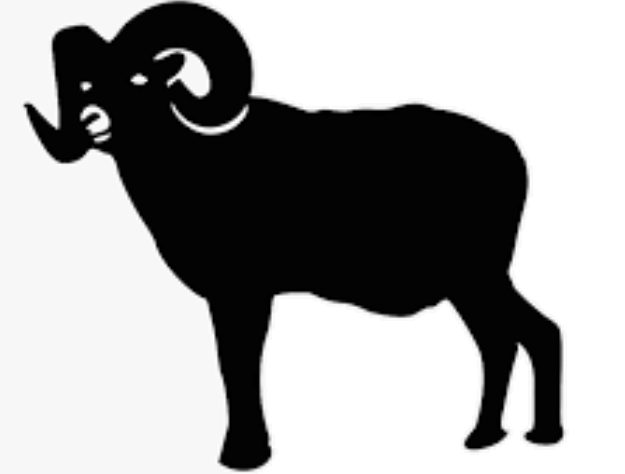
\includegraphics[width=2cm]{images/baran.png}}
\begin{song}{title={Świecie nasz}, music={Jan Kanty Pawluśkiewicz}, lyrics={Marek Grechuta}, annex}
\begin{multicols}{2}
    \begin{intro}
        \writechord{g} \writechord{F} \writechord{Eb} \writechord{d}
    \end{intro}
    \begin{verse}
        ^{g} Pytać zawsze --- ^{F}dokąd, dokąd \\
        ^{Eb} Gdzie jest prawda, ^{d}ziemi sól \\
        ^{g} Pytać zawsze --- ^{F}jak zagubić \\
        ^{Eb} Smutek wszelki, ^{d}płacz i ból
    \end{verse}
    \begin{verse}
        ^{g} Chwytać myśli n^{F}agłe, jasne \\
        ^{B} Szukać tam, gdzie świ^{F/A}atła biel \\
        |: ^{g} W Twoich oczach d^{F}wa ogniki | \\
        | ^{Eb} Już zwiastują, z^{d}naczą cel :|
    \end{verse}
    \begin{verse*}
        \writechord{g} \writechord{F} \writechord{Eb} \writechord{d} \\
        \writechord{g} \writechord{F} \writechord{Eb} \writechord{d} \\
        \writechord{g}
    \end{verse*}
    \begin{interlude}
        ^{a} Świecie nasz, ^{g}świecie nasz \\
        Chcę być z Tobą w ^{d}zmowie \\
        ^{F} Z blaskiem Twym, ^{d6}siłą twą \\
        Co mi dasz? Odp^{asus2}owiedz ^{A}
    \end{interlude}
    \begin{info}
        Świecie nasz --- daj nam \\
        Daj nam wreszcie zgodę \\
        Spokój daj --- zgubę weź \\
        Zabierz ją, odprowadź
    \end{info}
    \begin{info}
        Szukaj dróg gdzie jasny dźwięk \\
        Wśród ogni złych co budzą lęk \\
        Nie prowadź nas, powstrzymaj nas \\
        Powstrzymaj nas w pogoni\ldots
    \end{info}
    \begin{chorus}
        ^{F}Świecie ^{C}nasz \\
        Daj nam wi^{d}ele jasnych dni \\
        ^{a}Świecie n^{F}asz \\
        Daj nam w j^{G}asnym dniu oczekiwanie \medskip \\
        Świecie nasz \\
        Daj ugasić ogień zły \\
        Świecie nasz \\
        Daj nam radość, której tak szukamy \\
        Świecie nasz \\
        Daj nam płomień, stal i dźwięk \\
        Świecie nasz \\
        Daj otworzyć wszystkie ciężkie bramy \\
        Świecie nasz \\
        Daj pokonać każdy lęk \\
        Świecie nasz \\
        Daj nam radość blasku i odmiany! \\
        Świecie nasz \\
        Daj nam cień wysokich traw \\
        Świecie nasz \\
        Daj zagubić się wśród drzew poszumu \\
        Świecie nasz \\
        Daj nam ciszy czarny staw \\
        Świecie nasz \\
        Daj nam siłę krzyku, śpiewu tłumu \\
        Świecie nasz \\
        Daj nam wiele jasnych dni \\
        Świecie nasz \\
        Daj nam w jasnym dniu oczekiwanie \\
        Świecie nasz \\
        Daj ugasić ogień zły \\
        Świecie nasz
    \end{chorus}
    \begin{outro}
        Świecie nasz, świecie nasz \\
        Chcę być z tobą w zmowie \\
        Z blaskiem twym, z siłą twą \\
        Co mi dasz? Odpowiedz
    \end{outro}
\end{multicols}
\end{song}
\newpage\pagestyle{poezja}
\newpage
\begin{song}{title={Wilcza zamieć}, music={Marcin Przybyłowicz (z gry Wiedźmin: Dziki Gon)}, interpret={Studio Accantus}}
    \begin{intro}
        \writechord{d} \writechord{d} \writechord{B} \writechord{C} $\times 2$
    \end{intro}
    \begin{verse}
        Na ^{d}szlak moich blizn po^{B}prowadź ^{C}palec \\
        By ^{d}nasze drogi spleść ^{g}gwiazdom na ^{A}przekór \\
        ^{B} Otwórz te rany, ^{g} a potem ^{A}zalecz \\
        ^{d}Aż w zawiły losu ułożą się wzór
    \end{verse}
    \begin{chorus}
        Z moich ^{d}snów uciekasz nad ranem \\
        Cierpka ^{B}jak agrest, słodka jak bez ^{C} \\
        Chcę ^{d}śnić czarne loki splątane \\
        ^{B}Fiołkowe oczy ^{g}mokre od ^{A}łez
        \\
    \end{chorus}
    \begin{verse}
        Za wilczym śladem podążę w zamieć \\
        I twoje serce wytropię uparte \\
        Przez gniew i smutek stwardniałe w kamień \\
        Rozpalę usta smagane wiatrem
    \end{verse}
    \begin{chorus}
        Z moich snów uciekasz nad ranem\ldots
    \end{chorus}
    \begin{verse}
        Nie wiem czy jesteś moim przeznaczeniem \\
        Czy przez ślepy traf miłość nas związała \\
        Kiedy wyrzekłem moje życzenie \\
        Czyś mnie wbrew sobie wtedy pokochała?
    \end{verse}
    \begin{chorus}
        Z moich snów uciekasz nad ranem\ldots
    \end{chorus}
    \begin{interlude}
        \writechord{d} \writechord{d} \writechord{B} \writechord{C} $\times 2$
    \end{interlude}
\end{song}


\newpage
\begin{song}{title={Wild Mountain Thyme (Will Ye Go Lassie Go)}, music={tradycyjna}, interpret={The Corries}}
    \begin{verse}
        Oh the ^{D}summer t^{G}ime has c^{D}ome  \\
        And the tr^{G}ees are sweetly blo^{D}oming \\
        The w^{G}ild mo^{D}untain th^{h}yme \\
        Grows ar^{e}ound the blooming he^{G}ather \\
    \end{verse}
    \begin{chorus}
        Will ye g^{D}o, La^{G}ssie, g^{D}o? \\
        And we'll ^{G}all go toge^{D}ther \\
        To pull ^{G}wild mo^{D}untain th^{h}yme \\
        All ar^{e}ound the blooming he^{G}ather \\
        Will ye ^{D}go, ^{G}Lassie, ^{D}go? \\
    \end{chorus}
    \begin{verse}
        I will build my love a bower \\
        By yon' cool crystal fountain \\
        And 'round it I will pile \\
        All the wild flowers of the mountain \\
    \end{verse}
    \begin{chorus}
        Will ye go, Lassie, go? \ldots
    \end{chorus}
    \begin{verse}
        If my true love she'll not come \\
        Then I'll surely find another \\
        To pull wild mountain thyme \\
        All around the blooming heather \\
    \end{verse}
    \begin{chorus}
        Will ye go, Lassie, go? \ldots
    \end{chorus}
\end{song}



\chapter{Pop}
\begin{center}
    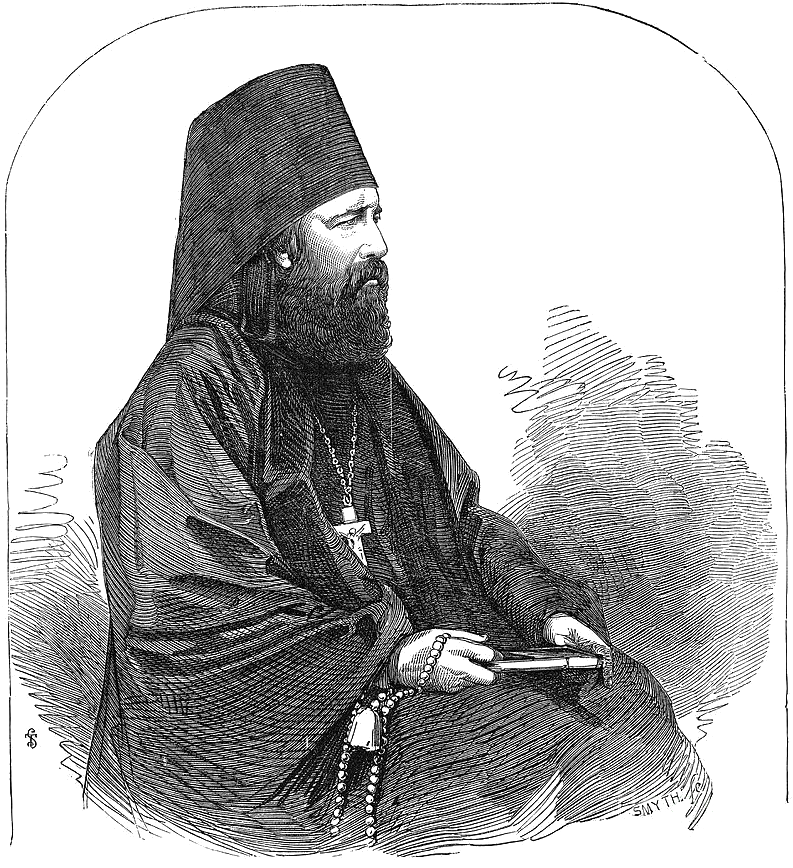
\includegraphics[width=0.4\textwidth]{images/pop.png}
\end{center}
\pagestyle{pop}
\newpage
\begin{song}{title={Byłaś serca biciem}, music={Jerzy Dobrzyński}, interpret={Andrzej Zaucha}, capo=3}
    \begin{intro}
    \writechord{a} \writechord{G} \writechord{d7} \writechord{d7}
    \end{intro}
    \begin{chorus}
        ^{a}Byłaś serca b^{G}iciem ^{d7} \\
        ^{a}Wiosną, zimą, ż^{G}yciem ^{d7} \\
        ^{a}Marzeń moich e^{G}chem ^{d7} \\
        ^{a}Winem, wiatrem, śmi^{G}echem ^{d7}
    \end{chorus}
    \begin{verse}
        Ostatnio w ^{a}mieście mym tramwaje ^{G}po północy b^{d7}łądzą \\
        Rozkładem n^{a}ocnych tras piekielne ^{G}jakieś moce rz^{d7}ądzą \\
        Nie wiedzieć ^{a}czemu wciąż rozkł^{G}ady jazdy ta^{d7}k zmieniają \\
        Że prawie k^{a}ażdy tramwaj ^{G}pod twym oknem ^{d7}nocą staje
    \end{verse}
      \begin{chorus}
        Byłaś serca biciem\ldots
    \end{chorus}
    \begin{verse}
        Ostatnio słońca mniej, ostatnio noce bardziej ciemne \\
        Już nawet księżyc drań o tobie nie chce gadać ze mną \\
        W kieszeni grosze dwa, w kieszeni na dwa szczęścia grosze \\
        W tym jednak losu żart, że ja obydwa grosze noszę
    \end{verse}
    \begin{chorus}
        Byłaś serca biciem\ldots
    \end{chorus}
    \begin{interlude}
        ^{F}Ktoś p^{d7}ytał jak się m^{C}asz, j^{a}ak się czujesz \\
        ^{F}Ktoś, z k^{d7}im rok w wojnę g^{C}rasz wycze^*{e}ku ^{A}je \\
        ^{F}Ktoś, k^{d7}to nocami, u^{C}licami, t^{a}ramwajami \\
        ^{F}Pod twe okno ^{d7}mknie, gdzie spo^*{D}ty ^{Eb}ka ^{E}mnie
    \end{interlude}
    \begin{chorus}
        Byłaś serca biciem\ldots
    \end{chorus}
    \begin{interlude}
        Ktoś pytał jak się masz\ldots
    \end{interlude}
\end{song}


\newpage
\begin{song}{title={Biała armia}, music={Bajm}, lyrics={Beata Kozidrak}}
    \begin{multicols}{2}
    \begin{intro}
    \writechord{c#} \writechord{E} \writechord{H} \writechord{A} $\times 2$\\ \\
    (\textit{bas cały czas E}) \\
    \writechord{e} \writechord{D} \writechord{e} \writechord{A} \\ 
    \writechord{e}   \writechord{A}
    \end{intro}
    \begin{verse}
        (\textit{kontynuuj riff z drugiej części intra}) \\
        To Twoja flaga, nasz młody przyjacielu \\
        Nie musisz kochać jej barw, o nie \\
        To Twoja armia i życie w ciągłym biegu \\
        Nigdy nie będziesz już sam \\ \\
        ^{e}Możesz wr^{D/F#}eszcie zachł^{G}ysnąć się ^{A}powietrzem \\
        I ^{e}unieść do g^{D/F#}óry jak pt^{A}ak, hej-he^{e}j \\
        Możesz wr^{D/F#}eszcie z^{G}abłądzić w wielkim m^{A}ieście \\
        Urodz^{e}iłeś się, by s^{D/F#}łużyć na^{A}m \\
    \end{verse}
    \begin{interlude}
        -----^{h}---  -----^{f#}--- Wła^{G}śnie nadszedł ten cz^{D}as \\
        -----^{h}---  -----^{f#}---   -----^{G} Who^{D}aaoh \\
         to jest wł^{h}aśnie t^{f#}en cz^{G}a - a - a^{D}s \\
    \end{interlude}
    \begin{interlude}
        \writechord{h} \writechord{A} \\
        \writechord{E} 
        \columnbreak
    \end{interlude}
    \begin{chorus}
        Jesteś s^{c#}terem, białym żołni^{E}erzem \\
        Nosisz sp^{H}odnie, więc w^{A}alcz \\
        Jesteś ża^{c#}glem, szalonym wi^{E}atrem \\
        Twoja s^{H}iła to ska^{A}rb         \\
    \end{chorus}
    \begin{verse}
        ^{N.C}Bóg jest z nami \\ \\
        ^{e}Jego pr^{D/F#}awda \\
        Jak t^{G}arcza Cię oca^{A}li \\
        Czek^{e}ałeś na t^{D}en dzień tyle l^{A}at \\
        ^{e}Ruszaj z n^{D/F#}ami, z wą^{G}tłymi marzen^{A}iami \\
        Z uf^{e}nością, k^{D}tórą jes^{A}zcze masz \\
    \end{verse}
    \begin{interlude}
        Właśnie nadszedł ten czas \ldots
    \end{interlude}
    \begin{chorus}
        Jesteś sterem, białym żołnierzem \ldots
    \end{chorus}
    \begin{solo}
        \textit{(akordy jak w drugiej części intra)}
    \end{solo}
    \begin{chorus}
        Jesteś sterem, białym żołnierzem \ldots  $\times 2$\\
    \end{chorus}
    \end{multicols}
\end{song}


\newpage
\begin{song}{title={C'est la vie (Paryż z pocztówki)}, music={Wiesław Pieregorólka}, lyrics={Jacek Cygan}, interpret={Andrzej Zaucha}}
    \begin{multicols}{2}
    \begin{intro}
    \writechord{B} \writechord{F/A} \writechord{g7} \writechord{C} \writechord{F} \writechord{F7/A} \\ 
    \writechord{B} \writechord{F/A} \writechord{g7} \writechord{g7/C} \\
    \writechord{F} \writechord{B/F} \writechord{F} \writechord{F7/A}
    \end{intro}
    \begin{verse}
        ^{B}C'est la v^{F/A}ie \\
        Cały Twój P^{g7}aryż z pocz^{C}tówek i ^{F}mgły --^{F7}- \\
        ^{B}C'est la v^{F/A}ie \\
        Wymyślon^{g7}y --^{g7/C}-  \\
        ^{B}C'est la v^{F/A}ie \\
        Ciebie obch^{g7}odzi, przejmu^{g7/C}jesz się ty^{F}m \\
    \end{verse}
    \begin{intro}
        \textit{play intro again}
    \end{intro}
    \begin{verse}
        ^{B}C'est la v^{F/A}ie \\
         Podmiejski po^{g7}ciąg rozw^{C}ozi Twe d^{F}ni --^{F7}- \\
        ^{B}C'est la v^{F/A}ie \\
         Wciąż spóź^{g7}niony --^{g7/C}-  \\
        ^{B}C'est la v^{F/A}ie \\
         Cały Twój P^{g7}aryż, dwie dr^{C}ogi na kr^{F}zyż --^{F7}- \\ 

        ^{B}Knajpa, ko^{F/A}ściół -^{g7}-- wi^{g7/C}dok z mo^{F}stu --^{F7} \\
        ^{B}Knajpa, ko^{F/A}ściół i ten b^{g7}ruk - i^{g7/C}deał nie tknął g^{F}o \\ 
    \end{verse}
    \begin{interlude}
        \writechord{F} \writechord{F/A} \\
        \writechord{B} \writechord{B/G} \writechord{B/C} $\times 2$
    \end{interlude}
    \begin{verse}
        ^{B}Knajpa, ko^{F/A}ściół -^{g7}-- wi^{g7/C}dok z mo^{F}stu --^{F7} \\
        ^{B}Knajpa, ko^{F/A}ściół i ten b^{g7}ruk - tak re^{g7/C}alny \\ 
    \end{verse}
    \begin{chorus}
        ^{C#}Zostaniesz t^{G#/C}u - ile m^{b7}ożna tak ż^{Eb}yć na pa^{G#}lcach -^{G#7}-- \\
        ^{C#}Zostaniesz t^{G#/C}u - po złud^{b7}zenia -^{b7/Eb}-- \\
        ^{H}Zostaniesz t^{F#}u - w "Kaskadzie" n^{g#7}ocą też gr^{C#7}ają wa^{F#}lca \\
        ^{H}Już na rogu ku^{F#}mple, jak grzech \\
        -^{g#}-- Odwr^{C#}otu już ni^{F#}e ma \\
        Nie, n^{F#7}ie nie \\
        ^{H}Wypijesz to wsz^{F#}ystko do dna, także dz^{g#7}iś \\
        ^{g#7/c#}Jak c^{H}o dnia \\
    \end{chorus}
    \begin{interlude}
        \writechord{H} \writechord{F#/B} \writechord{g#7} \writechord{C#} \writechord{F#} \writechord{F#7/B} \\ 
        \writechord{H} \writechord{F#/B} \writechord{g#7} \writechord{g#7/C#} \\
        \writechord{F#} \writechord{H/F#} \writechord{F#} \writechord{F#7/B}
    \end{interlude}
    \begin{verse}
        \textit{(akordy jak na początku tylko pół tonu wyżej)}
        C'est la vie \\
        Cały Twój Paryż z pocztówek i mgły \\
        C'est la vie \\
        Wymyślony  \\
        C'est la vie \\ 
        Cały Twój Paryż, dwie drogi na krzyż \\ 
        Knajpa, kościół - widok z mostu \\
        Knajpa, kościół i ten bruk - ideał nie tknął go \\
    \end{verse}
    \end{multicols}
\end{song}


\newpage
\begin{song}{title={Co mi Panie dasz}, music={Bajm}, lyrics={Beata Kozidrak}}
    \begin{intro}
    \writechord{h} \writechord{A} \writechord{G} \writechord{F#}
    \end{intro}
    \begin{verse}
        ^{h}Karuzela gna, w głośnikach wciąż muzy^{A}ka gra \\
        ^{G}Czuję, jak w jej takt kołyszę się ca^{F#}ła \\
        I raz, i dwa, i trzy, i w górę serca, wielki czis \\
        Czujność śpi, trochę mdli, jak szarlotka z rana \\
    \end{verse}
    \begin{chorus}
        Co mi, P^{h}anie, dasz w ten niep^{A}ewny czas? \\
        Jakie sł^{G}owa ukołyszą moją duszę, moją przyszłość \\
        Na tę re^{F#}sztę lat? \\
        Kilka sta^{h}rych szmat bym na ty^{A}łku siadł \\
        I czy w^{G}arto, czy nie warto mocną wódę leję w gardło \\
        By uk^{F#}oić żal \\
    \end{chorus}
    \begin{verse}
        Co tam nagi brzuch i w górę połatany ciuch \\
        Czuję ten wiatru pęd aż głowa odpada \\
        I raz, i dwa, i trzy, i wcale nie jest zimno mi \\
        Z góry pluć, gumę żuć tu wszystko wypada \\
    \end{verse}
    \begin{chorus}
        Co mi Panie dasz...
    \end{chorus}
\end{song}


\newpage
\begin{song}{title={Granda}, music={Monika Brodka}}
	\begin{intro}
	\writechord{e} \writechord{e} \writechord{H} \writechord{A} $\times 2$ \\
		Ni^{e}e polubię cię \\
		Jak powiedzieć prościej \\
		Zbl^{H}iżysz się o krok, porach^{A}uję kości \\
		Ni^{e}e polubię cię \\
		Twej koszuli pstrości \\
		Zbl^{H}iżysz się o krok, porach^{A}uję kości
	\end{intro}
	\begin{verse}
		\textit{riff:} \writechord {e5} \writechord{h5} \writechord{d5} \writechord{a5} \\	\\
		Kusisz zapachami \\
		Prowokujesz gestem \\
		Wodzisz za mną wzrokiem \\
		Czterogłowym smokiem \\
		Namierzasz radarami \\
		Jestem jak ruchomy cel \\
		Naostrzone zęby \\ 
		Nie polubię cię 
	\end{verse}
	\begin{chorus}
		Ni^{e}e polubię cię \\
		Jak powiedzieć prościej \\
		Zbl^{H}iżysz się o krok, porach^{A}uję kości \\
		Ni^{e}e polubię cię \\
		Twej koszuli pstrości \\
		Zbl^{H}iżysz się o krok, porach^{A}uję kości \\
		Do pięciu liczę, znikaj \\
		Dwa, trzy, cztery, pięć \\ 
		Raz, dwa, trzy, cztery, pięć \\
		Nie będzie dziś walczyka \\ 
		Dwa, trzy, cztery, pięć \\
		Raz, dwa, trzy, cztery, pięć \\
	\end{chorus}
	\begin{verse}
		Tropią mnie zwiadowcy \\
		Węszą myśliwskie psy \\
		Jak dziką zwierzynę \\
		Co kruszeje żywcem \\
		Zastawiłeś sidła \\
		Zmieniłeś zasady gry \\ 
		Zablokowałeś drogi \\
		Zaryglowałeś drzwi
	\end{verse}
	\begin{chorus}
		Nie polubię cię \ldots $\times 2$
	\end{chorus}
\end{song}


\newpage
\begin{song}{title={Hydropiekłowstąpienie}, music={Lao Che}, capo=2, annex}
\small
\begin{multicols}{2}
    \begin{intro}
        \writechord{e5} \writechord{G5} \writechord{C5} \writechord{H5}
    \end{intro}
    \begin{riff}
        \writechord{e} \writechord{H7} \writechord{e} \writechord{H7} $\times 8$
    \end{riff}
    \begin{verse}
        Słuchaj, Noe, chciałbym na słówko \smallskip \\
        Wiesz, tak między nami, to \\
        Jestem człowiekiem zaniepokojony \\
        By rzec: rozczarowany \smallskip \\
        Bo miałem ambicję stworzyć \\
        Taką rezolutną rasę \smallskip \\
        A wyście to tak po ludzku \\
        Po ludzku, spartolili \smallskip \\
        Jestem piekielnie sfrustrowany
    \end{verse}
    \begin{interlude}
        Płyń, płyń, Noe, płyń i żyj, a utop to, kim byłeś \\
        Płyń, płyń, Noe, płyń i żyj, jak nawet nie śniłeś
    \end{interlude}
    \begin{verse}
        Wiesz sam, jak nie lubię radykałów \smallskip \\
        Ale, na Boga, nie spałem całą noc \\
        I podjąłem decyzję \smallskip \\
        Zsyłam na Ziemię potop \\
        Mój mały Noe \smallskip \\
        Mój ptysiu miętowy, zsyłam potop \\
        Potop!
    \end{verse}
    \begin{riff}
        \writechord{e} \writechord{H7/F#} \writechord{G} \writechord{H7/F#}
    \end{riff}
    \begin{chorus}
        Utopię waszą utopię \\
        Utopię waszą utopię, ja\ldots \smallskip \\
        Utopię waszą utopie \\
        Utopię w potopie \\
        Zarządzam pełne zanurzenie \smallskip \\
        Utopię waszą utopie \\
        Utopię w potopie \\
        Hydropiekłowstąpienie
    \end{chorus}
    \begin{verse}
        Zatem, utonie wszystko: \smallskip \\
        Drogi i mosty kołowe \\
        Urzędy skarbowe \\
        Gospodarstwa domowe \smallskip \\
        Powiadam: wszystko \\
        Za wyjątkiem ciebie, chłopaku \\
        Wypływasz jutro \\
        Mandżur pakuj!
    \end{verse}
    \begin{chorus}
        Utopię waszą utopię\ldots
    \end{chorus}
    \begin{interlude}
        \writechord{e5} \writechord{G5} \writechord{C5} \writechord{H5} $\times 4$ \medskip \\
        Płyń, płyń, Noe, płyń i żyj, a utop to, kim byłeś \\
        Płyń, płyń, Noe, płyń i żyj, jak nawet nie śniłeś
    \end{interlude}
    \begin{verse}
        Wybrałem ciebie, bo\ldots \\
        Tak właściwie, to nie wiem \\
        Dlaczego ciebie wybrałem \smallskip \\
        Chciałem tylko, żebyś był fajny \\
        I żeby ktoś kiedyś mógł powiedzieć: \smallskip \\
        \say{Był Noe \\
        Noe --- gość, co się czasem spinał \smallskip \\
        Ale uwierzył, i gdy szedł po gnoju \\
        Smród już się go nie imał!}
    \end{verse}
    \begin{chorus}
        Płyń, chłopaku, płyń \\
        Płyń, nie odwracaj główki chłopaku, ty płyń \\
        A ja\ldots \smallskip \\
        Utopię waszą utopię \\
        Utopię w potopie \\
        Zarządzam pełne zanurzenie \smallskip \\
        Utopię waszą utopię \\
        Utopię w potopie \\
        Hydropiekłowstąpienie \medskip \\
        \writechord{e5} \writechord{G5} \writechord{C5} \writechord{H5} $\times 2$
    \end{chorus}
\end{multicols}
\end{song}


\newpage
\small
\begin{song}{title={In the End}, music={Linkin Park}, capo={1}}
    \begin{intro}
        \writechord{d} \writechord{C} \writechord{B} \writechord{C} $\times 2$
    \end{intro}
    \begin{multicols}{2}
    \begin{verse}
        \textit{(It starts with\ldots)} \\
        ^{d}One thing, I don't know why \\
        It ^{C}doesn't even matter how hard you try \\
        Ke^{B}ep that in mind, I designed this rhyme \\
        To expla^{C}in in due time \textit{(all I know)} \\
        Time is a valuable thing \\
        Watch it fly by as the pendulum swings \\
        Watch it count down to the end of the day \\
        The clock ticks life away \textit{(it's so unreal)} \\
        Didn't look out below \\
        Watch the time go right out the window \\
        Tryin' to hold on, I didn't even know \\
        I wasted it all, just to\ldots \textit{(watch you go)} \\
        I kept everything inside \\
        And even though I tried, it all fell apart \\
        What it meant to me will eventually be \\
        A memory of a time, when\ldots
    \end{verse}
    \begin{chorus}
        I tried so ^{d}hard and got so f^{F}ar \\
        But in the e^{C}nd, it doesn't even ma^{B}tter \\
        I had to ^{d}fall to lose it a^{F}ll \\
        But in the e^{C}nd, it doesn't even ma^{B}tter
    \end{chorus}
    \vfill\null\columnbreak{}
    \begin{verse}
        One thing, I don't know why \\
        It doesn't even matter how hard you try \\
        Keep that in mind, I designed this rhyme \\
        To remind myself how\ldots \textit{(I tried so hard)} \\
        In spite of the way you were mockin' me \\
        Actin' like I was part of your property \\
        Rememberin' all the times you fought with me \\
        I'm surprised it\ldots \textit{(got so far)} \\
        Things aren't the way they were before \\
        You wouldn't even recognize me anymore \\
        Not that you knew me back then \\
        But it all comes back to me \textit{(in the end)} \\
        You kept everything inside \\
        And even though I tried, it all fell apart \\
        What it meant to me will eventually be \\
        A memory of a time when\ldots
    \end{verse}
    \begin{chorus}
        I tried so hard and got so far\ldots
    \end{chorus}
    \begin{interlude}
        I've put my tr^{d}ust in yo^{C}u \\
        Pushed as f^{B}ar as I can g^{C}o \\
        For all th^{d}is, there's only o^{C}ne thing you should ^*{B}kn ^{C}ow
    \end{interlude}
    \begin{info}
        \textit{(mocniej, głośniej, \textbf{drzeć ryja})} \\
        I've put my tr^{d}ust in yo^{F}u \\
        Pushed as f^{C}ar as I can g^{B}o \\
        For all th^{d}is, there's only o^{F}ne thing you should ^*{C}kn ^{B}ow
    \end{info}
    \begin{chorus}
        I tried so hard and got so far\ldots
    \end{chorus}
    \begin{interlude}
        \writechord{d} \writechord{C} \writechord{B} \writechord{C} $\times 2$
    \end{interlude}
    \end{multicols}
\end{song}


\newpage
\fancyfoot[LO,RE]{
\includegraphics[height=45pt]{images/smok.png}}
\begin{song}{title={I See Fire}, music={Ed Sheeran}}
    \small
    \begin{intro}
        ^{a}Oh, misty eye of the mountain below \\
        Keep careful watch of my brothers' souls \\
        And should the sky be filled with fire and smoke \\
        Keep watching over Durin's sons
    \end{intro}
    \begin{verse*}
        \writechord{a} \writechord{F} \writechord{G} \writechord{a} $\times 2$
    \end{verse*}
    \begin{multicols}{2}
    \begin{verse}
        If this is to e^{a}nd in f^{C}ire \\
        Then we should ^{G}all burn ^{F} together \\
        Watch the ^{a}flames climb ^{C}high \\
        ^{G}Into the ^{d7}night \smallskip \\
        Calling ^{a}out fat^{C}her, oh \\
        ^{G}Stand by and ^{F}we will \\
        Watch the ^{d7}flames burn ^{C/E}auburn on \\
        The ^{F}mountain side, high\ldots
    \end{verse}
    \begin{verse*}
        \writechord{a} \writechord{F} \writechord{G} \writechord{a}
    \end{verse*}
    \begin{verse}
        And if we should die tonight \\
        Then we should all die together \\
        Raise a glass of wine \\
        For the last time \smallskip \\
        Calling out father, oh \\
        Prepare as we will \\
        Watch the flames burn auburn on \\
        The mountain side \medskip \\
        Desol^{d7}ation ^{C/E}comes upon the s^{F}ky
    \end{verse}
    \begin{chorus}
        Now I see ^{a}fire ^{F} ^{G}inside the ^{a}mountain \\
        I see ^{a}fire ^{F} ^{G}burning the ^{a}trees \\
        And I see ^*{a}fi ^{F}re ^{G}hollowing ^{a}souls \\
        I see ^*{a}fi ^{F}re, bl^{G}ood in the ^{a}breeze \bigskip \\
        And I hope that you remember me
    \end{chorus}
    \begin{verse*}
        a F G a $\times 2$
    \end{verse*}
    \vfill\null\columnbreak{}
    \begin{verse}
        Oh, should my people fall \\
        Then surely I'll do the same \\
        Confined in mountain halls \\
        We got too close to the flame \smallskip \\
        Calling out father, oh \\
        Hold fast and we will \\
        Watch the flames burn auburn on \\
        The mountain side \smallskip \\
        Desolation comes upon the sky
    \end{verse}
    \begin{chorus}
        Now I see fire inside the mountain\ldots
    \end{chorus}
    \begin{interlude}
        And if the ^{d7}night is ^{a}burning \\
        I will ^{C}cover my ^{G}eyes \\
        For if the ^{d7}dark re^{a}turns \\
        Then my ^{C}brothers will ^{G}die \smallskip \\
        And as the ^{d7}sky is falling ^{a}down \\
        It crashed in^{C}to this lonely ^{G}town \\
        And with that ^{d7}shadow upon the ground \\
        I ^{C/E}hear my ^{F}people screaming o^{G}ut
    \end{interlude}
    \begin{chorus}
        Now I see fire inside the mountain \\
        I see fire burning the trees \\
        And I see fire hollowing souls \\
        I see fire, blood in the breeze
    \end{chorus}
    \begin{chorus*}
        I see fire \\
        \textit{Oh, you know I saw a city burning out} \smallskip \\
        And I see fire \\
        \textit{Feel the heat upon my skin, yeah} \smallskip \\
        And I see fire \\
        \textit{Ooh ooh ooh ooh} \smallskip \\
        And I see fire burn auburn on the mountain side
    \end{chorus*}
    \end{multicols}
\end{song}

\newpage\pagestyle{pop}
\newpage
\begin{song}{title={Kocham cię jak Irlandię}, music={Kobranocka}}
    \begin{multicols}{2}
    \begin{verse}
        Zni^{F}kałaś gdzieś w ^{Fmaj7}domu nad Wisłą \\
        Pa^{F7}miętam to tak do^{g}kładnie \\
        ^{Eb} Twoich czarnych ^{B}oczu bliskość \\
        Wciąż ^{F}kocham cię, jak Ir^{C}landię \smallskip \\
        A ^{F}ty się temu nie ^{Fmaj7}dziwisz \\
        Wiesz ^{F}dobrze, co byłoby ^{g}dalej \\
        ^{Eb} Jak byśmy ^{B}byli szczęśliwi \\
        G^{F}dybym nie ^{C}kochał cię ^{F}wcale \bigskip \\
        (\writechord{F}) \writechord{Fmaj7} \writechord{F7} \writechord{g} $\times 2$
    \end{verse}
    \begin{verse}
        Przed szczęściem żywić obawę \\
        W nadziei, że mi ją skradniesz \\
        Wlokę ten ból przez Włocławek \\
        Kochając cię, jak Irlandię \medskip \\
        A ty się temu nie dziwisz \\
        Wiesz dobrze, co byłoby dalej \\
        Jak byśmy byli szczęśliwi \\
        Gdybym nie kochał cię wcale
    \end{verse}
    \vfill\null\columnbreak{}
    \begin{info}
        \textit{(ton wyżej)}
    \end{info}
    \begin{verse}
        ^{G} Gdzieś na u^{Gmaj7}licy fabrycznej \\
        S^{G7}potkać się nam się wy^{a}padnie \\
        ^{F} Lecz takie są ^{C}widać wytyczne \\
        By ^{G}kochać cię, jak Ir^{D}landię \medskip \\
        A ty się temu nie dziwisz \\
        Wiesz dobrze, co byłoby dalej \\
        Jak byśmy byli szczęśliwi \\
        Gdybym nie kochał cię wcale
    \end{verse}
    \begin{info}
        \textit{(ton wyżej)}
    \end{info}
    \begin{verse}
        ^{A} Czy mi to ^{Amaj7}kiedyś wybaczysz \\
        Dzia^{A7}łałem tak niepo^{h}radnie \\
        ^{G} Czy to dla ^{D}ciebie coś znaczy \\
        Że ^{A}kocham cię, jak Ir^{E}landię \medskip \\
        A ty się temu nie dziwisz \\
        Wiesz dobrze, co byłoby dalej \\
        Jak byśmy byli szczęśliwi \\
        Gdybym nie kochał cię wcale
    \end{verse}
    \begin{interlude}
        \writechord{G}\writechord{A5} -- \writechord{G}\writechord{A5} -- \writechord{G}\writechord{A5} \\
        \writechord{h5} -- \writechord{C#5} \writechord{D5} \writechord{C#5} \writechord{h5} $\times 4$
    \end{interlude}
    \begin{outro}
        A ty się temu nie dziwisz \\
        Wiesz dobrze, co byłoby dalej \\
        Jak byśmy byli szczęśliwi \\
        Gdybym nie kochał cię wcale \medskip \\
        \writechord{A} \writechord{Amaj7} \writechord{A7} \\
        \writechord{h5} -- \writechord{C#5} \writechord{D5} \writechord{C#5} \writechord{h5} $\times 4$
    \end{outro}
    \end{multicols}
\end{song}


\newpage
\begin{song}{title={Kolorowy wiatr}, music={Alan Menken}, lyrics={Antoni Marianowicz}}
\small
    \begin{info}
        \writechord{N.C.} --- \say{No Chord}, pauza
    \end{info}
    \begin{multicols}{2}
    \begin{intro}
        \writechord{c} \\
        Ty m^{c}asz mnie za głupią dzi^{c/B}kuskę \\
        Lecz choć c^{c}ały świat zwiedziłeś \\
        Zj^{B}eździłeś wzdłuż i wszerz \\
        I m^{G#}ądry jesteś ^{N.C.}tak \\
        Że aż sł^{G#}ów podziwu br^{N.C.}ak \\
        Dla^{f}czego powiedz mi tak mało wi^{G}esz \\
        Mało wi^{C}esz ^{a} ^{C} ^{a}
    \end{intro}
    \begin{verse}
        Na l^{C}ądzie gdy rozglądasz się lą^{a}dując \\
        Chcesz wsz^{C}ystko mieć na własność, nawet gł^{e}az \\
        A ^{F}ja wiem, że ten głaz ma także d^{a}uszę \\
        Imię m^{d}a i zakl^{G}ęty w sobie cz^{a}as \smallskip \\
        Ty m^{C}yślisz, że są ludźmi tylko l^{a}udzie \\
        Których l^{C}udźmi nazywać chce twój świ^{e}at \\
        Lecz j^{F}eśli pójdziesz tropem moich br^{a}aci \\
        Dowiesz ^{d}się największych pr^{G}awd \\
        Najświętszych pr^{C}awd
    \end{verse}
    \vfill\null\columnbreak{}
    \begin{chorus}
        Czy wiesz, cz^{a}emu wilk tak wyje w księżyc^{e}ową n^{F}oc \\
        I cze^{a}mu ryś tak zęby szczerzy ra^{e}d?  \\
        Czy powt^{F}órzysz te mel^{G}odie, co z gór pł^{C}yną ^{a} \\
        Barwy, kt^{d7}óre kolorowy niesie wi^{G}atr \\
        Barwy, kt^{F}óre kolor^{G}owy niesie wi^{C}atr ^{a} ^{C} ^{a}
    \end{chorus}
    \begin{verse}
        \textit{(szybciej)} \\
        Pobiegnij za mną leśnych duktów szlakiem \\
        Spróbujmy jagód w pełne słońca dni \\
        Zanurzmy się w tych skarbach niezmierzonych \\
        I choć raz o ich cenach nie mów mi \smallskip \\
        Ulewa jest mą siostrą, strumień bratem \\
        A każde z żywych stworzeń to mój druh \\
        Jesteśmy połączonym z sobą światem \\
        A natura ten krąg życia wprawia w ruch
    \end{verse}
    \begin{interlude}
        Do ch^{F}mur każde dr^{e}zewo się pn^{a}ie \\
        Skąd to wi^{d}edzieć masz, skoro ści^{G}nasz je
    \end{interlude}
    \begin{chorus}
        To nie to^{a}bie ptak się zwierza w księży^{e}cową n^{F}oc  \\
        Lecz lu^{a}dziom wszelkich ras i wszelkich wi^{e}ar \\
        Chło^{F}nącym te mel^{G}odie, co z gór pł^{C}yną ^{a} \\
        Barwy, kt^{d7}óre kolorowy niesie wi^{G}atr \\
        Możesz zd^{d}obyć św^{e}iat, lecz to bę^{d}dzie ty^{e}lko świ^{F}at \\
        Tylko św^{a}iat --- nie barwy, które ^*{d7}nie ^{Gadd2}sie wi^{C}atr
    \end{chorus}
    \end{multicols}
\end{song}


\newpage
\small
\begin{song}{title={Małociasteczkowy}, music={Dawid Podsiadło}, interpret={808 Squad}}
\begin{multicols}{2}
    \begin{intro}
        (\textit{jęcząc}) \\
        H^{h}u hu hu hu hu hu h^{A}u hu h^{D}uuu, hu \\
        H^{E}u hu h^{f#}uuu, hu \\
        Hu hu h^{E}uuu, hu
    \end{intro}
    \begin{verse}
        Małociasteczk^{A}owa twarz \\
        ^*{E}Małoci astecz^{D}kowa głowa \\
        ^*{E}Małoci asteczk^{A}owy styl \\
        ^*{E}Małoci astecz^{D}kowo kocham \\
        Z ma^{h}łego ciasta wielkie sny  ^{A/C#} \\
        Atak^{D}ują twoje ulice ^{E}  \\
        Wyś^{f#}niłem sobie ciebie, gdy \\
        Śpiew^{E}ałem głośno pod prysznicem
    \end{verse}
    \begin{verse}
        Ten mój małociasteczkowy hit \\
        I małociasteczkowe słowa \\
        Ten małociasteczkowy rytm \\
        Melodia małociasteczkowa \\
        Z małego ciasta wielkie sny \\
        Gromadzą się na twoich ulicach \\
        Pamiętam, bardzo chciałem tu być \\
        Na pewno dużo bardziej niż dzisiaj
    \end{verse}
    \begin{chorus}
        Zn^{f#}owu jadę d^{E}o ciebie s^{A}am ^{h} \\
        Zn^{D}owu jadę do ciebi^{c#}e ^{E} $\times 4$
    \end{chorus}
    \begin{verse}
        Przez chwilę czułem się jak Bóg \\
        Przez chwilę byłem królem w cieście \\
        Wybrałem na siłownię strój \\
        I wtedy zrozumiałem wreszcie \\
        Że z mojego ciasta moje sny \\
        Budują twoje ulice \\
        Że ciebie nie zachwyca tu nic \\
        Ale smuci mnie, że nadal nie krzyczę
    \end{verse}
    \begin{verse}
        Gdy wielkomiejski piękny świat \\
        Na każdym kroku sypie kreski \\
        Uściski i klepnięcia w bark \\
        Płynące ze wzruszenia łezki \\
        Dlaczego wszystko sztuczne aż tak \\
        Że napromieniowane mi świeci \\
        Trzeba stąd wyjechać, bo strach \\
        Że wszystko przejdzie na moje dzieci
    \end{verse}
    \begin{interlude}
        Hu hu hu hu\ldots $\times 2$
    \end{interlude}
    \begin{chorus}
        Znowu jadę do ciebie sam \\
        Znowu jadę do ciebie $\times 3$
    \end{chorus}
    \begin{outro}
        H^{f#}u hu hu hu h^{E}u hu h^{A}uuu, hu \\
        H^{h}u hu hu^{D}uu, hu \\
        Hu hu h^{c#}uu hu ^{E} $\times 2$
    \end{outro}
\end{multicols}
\end{song}


\newpage
\small
\begin{song}{title={Miał być ślub}, music={Bartłomiej Kapłoński}, lyrics={Anna Dąbrowska}, interpret={Monika Brodka}} 
    \begin{intro}
        \writechord{D}
    \end{intro}
    \begin{verse}
        ^{D}Żoną miałam b^{D7}yć, miał być ś^{G}lub i we^{g}sele też \\
        Już ^*{D}zapro ^{f#/C#}siłam g^{H7}ości, kap^{e}ela z r^{e7/D}odzinnych st^{A/C#}ron \\
        ^{h}Miała tam gr^{A}ać ^{G}polkę na d^{F#}wa \\
        Matki ^*{h}pobłogosław ^{E/G#}iły dawno ^{A} nam ^{A7/G} ^{f#} ^{A/E}
    \end{verse}
    \begin{verse}
        Był umówiony ksiądz, bukiet mi przywieźli z białych róż \\
        Welon już na głowie, kościół pęka w szwach \\
        Babcia we łzach cichutko łka \\
        Organista daje znak, a jego brak
    \end{verse}
    \begin{chorus}
        Su^{D}kienka sa^{F#}motnie w szafie lś^{h}ni, nie zał^{E}oży jej już ni^{A}kt \\
        ^{E/G#} Nie dowie s^{f#}ię \\
        ^{h}Czemu ^{A}tak stało s^{E/G#}ię \\
        Zamiast \say{^{e}tak}, on po^{e6/D}wiedział \say{^{A}nie} \smallskip \\
        Zamó^{D}wiłam pog^{F#}odę na ten dzi^{h}eń, a i t^{E}ak znów padał d^{A}eszcz \\
        Nikt nie ^{E/G#}widział mych ł^{f#}ez \\
        ^{h}Gdy ^{A}mówiłeś, ż^{E/G#}e \\
        Nie po^{e}kochasz ^{e7/D}nigdy m^{A}nie na d^{f#}obre i złe
    \end{chorus}
    \begin{interlude}
        ^{C}Kto z miłości nie u^{G}marł nie potrafi ^*{D}żyć ^{A/C#} ^{H7} \\
        Moje ^{C}serce kiedyś zła^{G}mane mocniej kocha d^{D}ziś ^{A} \smallskip \\
        Kto z miłości jeszcze nie umarł nie potrafi żyć \\
        Moje serce kiedyś złamane mocniej kocha dziś
    \end{interlude}
\end{song}


\newpage
\begin{song}{title={Miłość, miłość}, music={Krzysztof Zalewski}}
    \begin{intro}
        \writechord{E} \writechord{D} \writechord{E} \writechord{D} \\
        \writechord{E} \writechord{D} \writechord{C} \writechord{A}
    \end{intro}
    \begin{multicols}{2}
    \begin{verse}
        ^{E} Bez ciebie wszystko mi j^{D}edno \\
        ^{E} I czuję, jakby mnie b^{D}yło pół \\
        Uparta chmura nade mną \\
        A chmura nade mną pozbawia mnie tchu
    \end{verse}
    \begin{verse*}
        Przy tobie ^{H} znika całe zło \\
        Przez otw^{D}arte okna \\
        Przy tobie ^{H} oddycham \\\
        Zapominam s^{D}ię na chwilę
    \end{verse*}
    \begin{chorus}
        ^{C}Ciebie więcej chcę, ^{e}musi mi to przejść \\
        I mi^{D}nąć mi miłość, i inne słowa \\
        Nie potrzebuję słów, mówiłem ci to już \\
        Dopłyną donikąd, to tylko słowa \\
        Ciebie więcej chcę, musi mi to przejść \\
        I minąć mi miłość, mijamy sobie
    \end{chorus}
    \begin{chorus*}
        \writechord{E} \writechord{D} \writechord{E} \writechord{D}
    \end{chorus*}
        \vfill\null\columnbreak{}
    \begin{verse}
        Czemu zatrzymać się nie da \\
        Tego momentu, gdy jesteś tuż \\
        Przy tobie znów chcę wszystkiego \\
        I jeszcze to wszystko mógłbym móc
    \end{verse}
    \begin{verse*}
        Przy tobie znika całe zło \\
        Przez otwarte okna \\
        Przy tobie oddycham \\
        Zapominam się na chwilę
    \end{verse*}
    \begin{chorus}
        Ciebie więcej chcę\ldots
    \end{chorus}
    \begin{interlude}
        \writechord{C} \writechord{e} \writechord{D} \writechord{D} \\
        Ooo o o\ldots $\times 2$
    \end{interlude}
    \begin{chorus}
        Ciebie więcej chcę, musi mi to przejść \\
        I minąć mi miłość, mijamy sobie
    \end{chorus}
    \begin{chorus*}
        \writechord{E} \writechord{D} \writechord{E} \writechord{D}
    \end{chorus*}
    \end{multicols}
\end{song}


\newpage
\begin{song}{title={Nie mam dla ciebie miłości}, lyrics={Basia „Flow“ Adamczyk}, music={Skubas}, capo=1}
    \begin{intro}
        \writechord{C} \writechord{a7} \writechord{e(b6)} $\times 2$
    \end{intro}
    \begin{verse}
        ^{C}Jeśli chcesz, może^{Cmaj7}sz przyjść, kupi^{G6}ć wino, zosta^{a7}ć na noc \\
        ^{C}Nie przytulę cię ^{Cmaj7}potem, od^{G6}wrócę, rzucę \say{do^{a7}branoc} \smallskip \\
        Jeśli chcesz, możesz przyjść, zdjąć bluzkę, zostać do rana \\
        Nie odprowadzę cię potem, do drzwi trafisz sama
    \end{verse}
    \begin{chorus}
        ^{C}Nie mam dla ciebie mi^{a7}łości, ^{e} ktoś tu był przed ^{e7}tobą \\
        ^{C}Nie ma we mnie mi^{a7}łości, od^{e}chodząc zabrała ją ze ^{e7}sobą
    \end{chorus}
    \begin{verse}
        Jeśli chcesz, troszcz się o mnie, tylko pozbądź się złudzeń \\
        Nie zacznę cię kochać, choć przy tobie się budzę \smallskip \\
        Jeśli chcesz, to dbaj o mnie, bądź zawsze pod ręką \\
        Jeśli pójdę z inną, nie mów -- serce ci pękło
    \end{verse}
    \begin{chorus}
        Nie mam dla ciebie miłości, ktoś tu był przed tobą \\
        Nie ma we mnie miłości, odchodząc zabrała ją ze sobą \smallskip \\
        Nie mam dla ciebie miłości, ktoś tu był przed tobą \\
        Nie ma we mnie miłości, odchodząc\ldots
    \end{chorus}
    \begin{interlude}
        \writechord{C} \writechord{a7} \writechord{e} \writechord{e} $\times 4$ \\
        \writechord{e} \writechord{e}
    \end{interlude}
    \begin{outro}
        Nie mam dla ciebie miłości\ldots \smallskip \\
        Nie ma we mnie miłości\ldots $\times 2$
    \end{outro}
    \begin{center}
        \vfill{}
        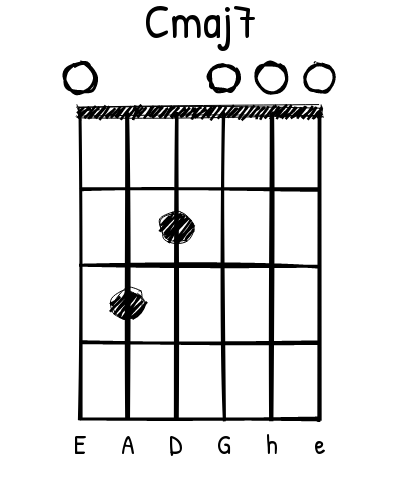
\includegraphics[height=3.5cm]{images/Cmaj7.png}
        \hspace{1cm}
        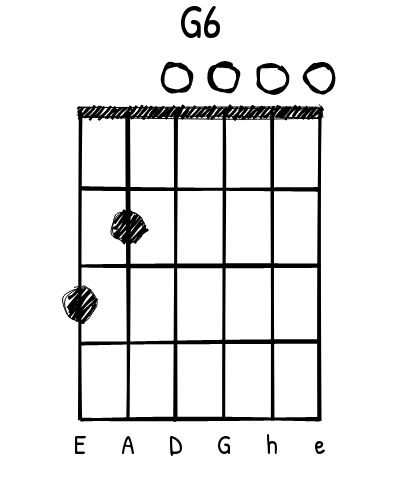
\includegraphics[height=3.5cm]{images/G6-easy.png}
        \vfill{}
    \end{center}
\end{song}


\newpage
\begin{song}{title={Pepe Pan Dziobak}, music={Marcin Szydłowski}, capo=3}
    \begin{intro}
        ^{e}Dubi dubi du-ła, dubi dubi du-ła \\
        ^{e}Dubi dubi du-ła, dubi dubi du-ła \\
        ^{H7}Pepe!
    \end{intro}
    \begin{verse}
        Oto ^{e}jaja znoszący ss^{C}ak, który rusza na a^{A7}kcję ^{C} \\
        Ten pie^{e}rzasty płaskostopiec do w^{C}alki wielki ma dr^{H7}y-yg! \\
        Oprócz w^{a}ielkich, płaskich stóp \\
        Ma bobrzy ^{e}ogon oraz dziób \\
        A ko^{a}biecy ród omdlewa na jego r^{H7}yk
    \end{verse}
    \begin{info}
        \textit{(odgłos dziobaka)}
    \end{info}
    \begin{chorus}
        To ^{e}Pepe! ^{C} Był tutaj i już z^{A7}nikł! ^{C} \\
        \textit{Możesz mówić \say{Agent P.}} \\
        ^{e}Pepe! ^{C} \\
        \textit{Powiedziałem, że możesz mówić \say{Agent P.}!}
    \end{chorus}
    \begin{chorus*}
        ^{H7}Agent P.!
    \end{chorus*}
\end{song}
\fancyfoot[LO,RE]{
\includegraphics[height=45pt]{images/pepe.png}}

\newpage\pagestyle{pop}
\newpage
\begin{song}{title={Piła tango}, music={Strachy na Lachy}}
    \normalsize
	\begin{intro}
	    \writechord{a} \writechord{a} \writechord{d} \writechord{E} $\times 3$ \\
        \writechord{a} \writechord{a} \writechord{d}
	\end{intro}
    \begin{verse*}
        Oto ^{E}historia z ^{a}kantem ^{d} \\
        Co pod^{E}wójne ma dn^{a}o ^{d} \\
        Gdyby na^{E}pisał ją ^{a}Dante ^{d} \\
        To nie ^{E}tak by to szł^*{a}o \ldots ^{d} ^{E}
    \end{verse*}
    \begin{verse}
        Grzesiek ^{a}Kubiak, czyli ``Kuba'', rządził ^{d}naszą podsta^{E}wówką \\
        Po ^{a}lekcjach na boisku ganiał ^{d}za mną z cegł^{E}ówką \\
        W Pile było jak w Chile, każdy miał czerwone ryło \\
        Mniej lub bardziej to pamiętasz --- spytaj jak to było \\
        W czasach, gdy nad Piłą jeszcze latały samoloty \\
        Wojewoda Śliwiński kazał pomalować płoty \\
        Potem wszystkie płoty w Pile miały kolor zieleni \\
        Rogaczem na wieżowcu Piła witała jeleni
    \end{verse}
    \begin{verse*}
        \writechord{E7}
    \end{verse*}
    \begin{chorus}
        Statek ^{a}Piła Tango ^{d7} ^{E7} \\
        Czar^{a}na bandera ^{d7} ^{E7} \\
        To tylko Piła tango \\
        Tańczysz to teraz \\
        Płynie statek Piła Tango \\
        Czarna bandera \\
        Ukłoń się świrom \\
        Żyj, nie umieraj
    \end{chorus}
    \newpage
    \begin{verse}
        Gruby jak armata Szczepan błąkał się po kuli ziemskiej \\
        Trafił do Ameryki prosto z Legii Cudzoziemskiej \\
        Baca w Londynie z Buchami się sąsiedzi \\
        Lżej się tam halucynuje, nikt go tam nie śledzi \\
        Karawan z Holandią przyjechał tutaj wreszcie \\
        Są już Kula, Czarny Dusioł --- słychać strzały na mieście \\
        Znam jednak takie miejsca, gdzie jest lepiej chodzić z nożem \\
        Całe Górne i Podlasie, wszyscy są za Kolejorzem (hej, Kolejorz!)
    \end{verse}
    \begin{chorus}
        Statek Piła Tango\ldots
    \end{chorus}
    \begin{verse}
        Andrzej Kozak, Mandaryn --- znana postać medialna \\
        Tyci przy nim jest kosmos, gaśnie Gwiazda Polarna \\
        Jest tu Siwy, który w rękach niebezpieczne ma narzędzie \\
        A kiedy Siwy tańczy, znaczy mordobicie będzie \\
        U Budzików Pod Tytułem chleją nawet z gór szkieły \\
        Zbigu śpi przy stoliku, ma nieczynny przełyk \\
        Lecz spokojnie, panowie, według mej najlepszej wiedzy \\
        Najszersze gardła tu to mają z INRI koledzy
    \end{verse}
    \begin{chorus}
        Statek Piła Tango\ldots
    \end{chorus}
    \begin{verse}
        Nad rzeką, latem ferajna na grilla się zasadza \\
        Auta z Niemiec? Sam wiem, kto je tu sprowadza \\
        Żaden spleen i cud, na ulicach nie śpią złotówki \\
        W Pile Święta jest Rodzina i święte są żarówki \\
        Nic nie szkodzi, że z wieczora miasto dławi się w fetorach \\
        Ważne, że jest żużel i kiełbasy senatora \\
        Fajne z Wincentego Pola idą w świat dziewczyny \\
        Po pokładzie jeździ Jojo bicyklem z Ukrainy
    \end{verse}
    \begin{chorus}
        Statek Piła Tango\ldots
    \end{chorus}
    \begin{interlude}
        Oto historia z kantem \\
        Co podwójne ma dno \\
        Gdyby napisał ją Dante \\
        To nie tak by to szło\ldots \\
        (by szło, by szło\ldots)
    \end{interlude}
\end{song}


\newpage
\fancyfoot[LO,RE]{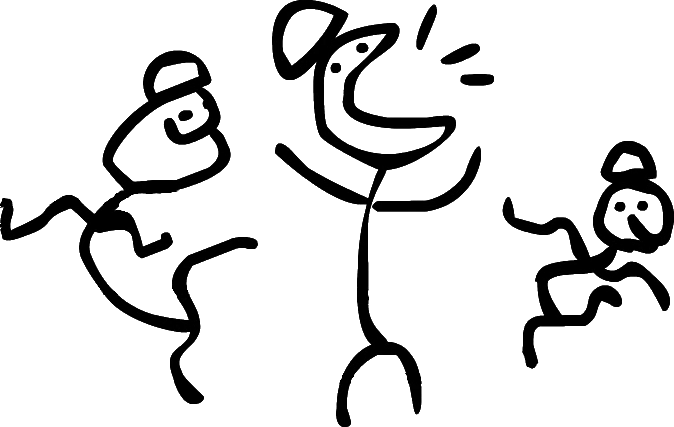
\includegraphics[height=45pt]{images/hutnicy.png}}
\begin{song}{title={Piosenka o hucie}, lyrics={Jakub \say{Dem3000} Dębski}, music={Romek Buga}, capo=1, annex}
    \begin{intro}
        \say{Czasami w hu^{Dmaj7}cie spotykamy się wszyscy i pracujemy tam \\
        A ^{e7}czasami nie, czasami śpiewamy piosenki, na przykład moją ulubio-- \\
        Moją ^{A7}ulubioną piosenkę} --- pomyślał sobie, przypomniał sobie swoją ulubioną piosenkę:
    \end{intro}
    \begin{chorus}
        ^{Dmaj7}Hej! ^*{h7} Otrzymy ^{e7}wanie me^{A7}tali \\
        Z r^{Dmaj7}ud i z^{h7}łomu ^{e7} ^{A7} \\
        To jest ^{Dmaj7}to, co ^{h7}lubię naj^{e7}bardziej ^{A7} \\
        To jest ^{Dmaj7}to, co ^{h7}lubię naj^{e7}bardziej \\
        ^{A7}Wytapiać sz^{Dmaj7}kło --- i prze^{h7}twarzać produkty sz^{e7}klane ^{A7} \\
        Praca w ^*{Dmaj7}hu--- ^*{h7}uc ^{e7}ie ^{A7} \\
        Praca w hu^{Dmaj7}cie
    \end{chorus}
\end{song}

\newpage\pagestyle{pop}
\newpage
\small
\begin{song}{title={Piosenka pisana nocą}, music={Coma}} 
    \begin{info}
		\writechord{Dadd4add9} - przesuń C-Dur dwa progi w prawo \\
		\writechord{A7sus4add6} - przesuń C-Dur dwa progi w prawo, połóż palec na 5 progu najgrubszej struny  
    \end{info}
    \begin{intro}
        \writechord{Fmaj7} \writechord{a} \\
    	\writechord{Dadd4add9} \writechord{A7sus4add6}
    \end{intro}
    \begin{verse}
    	^{Fmaj7} Zapomniałem nakr^{a}ęcić czas \\
		^{Dadd4add9} I zapomniałem rozpo^{A7sus4add6}cząć nowy dzień \\
		W zagubionej przestrzeni trwam \\
		Cały świat płynie obok gdzieś \\ \\
		A może ja jestem opowieść \\
		Zmęczonych ust \\
		Znudziłem się Bogu \\
		W połowie, w połowie 
	\end{verse}
	\begin{chorus}
		^{C}Nie ma już nic \\
		^{e}Nie ma już nic \\
		^{Dadd4add9}Nie ma już nic po ta^{A7sus4add6}mtej stronie \\
		Nie ma już nic \\
		Nie ma już nic \\
		Nie ma już nic za  ścianą powiek \\
	\end{chorus}
	\begin{verse}
		Nie potrafię dokończyć spraw \\
		I nie potrafię wypełnić własnych słów \\
		Jutro zginie ostatni ślad \\
		Zapomnicie że byłem tu \\
		A może ja jestem opowieść \\
		Zmęczonych ust \\
		Znudziłem się Bogu \\
		W połowie, w połowie 
	\end{verse}
	\begin{chorus}
		Nie ma już nic\ldots
	\end{chorus}
	\begin{interlude}
		^{e}Jeszcze raz ^{D} mógłbym zmi^{e}enić ksz^{D}tałt \\
		Rozpiąć skr^{e}zydła i fr^{D}unąć nie zważ^{e}ając na str^{D}ach \\
		^{e}Jeszcze raz, ^{D} przecież spo^{e}sób zn ^{D}am \\
		Tylko n^{e}ie mam już si^{D}ły \\
		Tylko ni^{e}e wiem ja^{D}k \\ \\
		\writechord{Fmaj7} \writechord{a} \\
    	\writechord{Dadd4add9} \writechord{A7sus4add6}
	\end{interlude}
	\begin{chorus}
		Nie ma już nic\ldots
	\end{chorus}
\end{song}


\newpage
\small
\begin{song}{title={Pomaluj moje sny}, music={Breakout}}
    \begin{info}
        (16-bar blues, A moll)
    \end{info}
    \begin{intro}
        \writechord{C} \writechord{C} \writechord{D} \writechord{D} \\
        \writechord{a5} \writechord{G} \writechord{a5} \writechord{G} $\times 2$
    \end{intro}
    \begin{multicols}{2}
    \begin{verse}
        ^{a5} Nie zazdroszczę łodzi żagla, kiedy wiatr ^{G} \\
        ^{a5} Gna po morzach ją dalekich, gna przez świat ^{G} \\
        ^{a5} Nie zazdroszczę ptakom skrzydeł, rybom płetw^{G} \\
        ^{a5} Bo najbardziej ponad wszystko pragnę mieć \\
        Pragnę ^{D5}mieć, ^{C} ^{D5} ^{C}pragnę ^{a5}mieć ^{G} ^{a5} ^{G}
    \end{verse}
    \begin{chorus}
        ^{C} Sny kolorowe, ^{D} pomaluj moje sny ^{a5} ^{G} ^{a5} ^{G}
    \end{chorus}
    \bigskip
    \begin{verse}
        Chcę zamieszkać w kolorowym mieście snu \\
        W kolorowym rwać ogrodzie bukiet bzów \\
        Dla dziewczyny kolorowej, która w pieśń \\
        Wszystkie barwy i odcienie umie wpleść \\
        Ja chcę śnić, ja chcę śnić
    \end{verse}
    \begin{chorus}
        Sny kolorowe, pomaluj moje sny
    \end{chorus}
    \begin{solo}
        (zwrotka + refren)
    \end{solo}
    \begin{verse}
        Tak, jak gdybym tego mało miał za dnia \\
        Tyle czerni w moich snach jest, tyle zła \\
        Daj mi proszę chociaż w nocy barwny sen \\
        Niech mi we śnie będzie jaśniej, niż jest w dzień \\
        Daj mi dziś, daj mi dziś
    \end{verse}
    \begin{chorus}
        Sny kolorowe, pomaluj moje sny $\times 4$
    \end{chorus}
    \vfill\null\columnbreak{}
    \begin{center}
      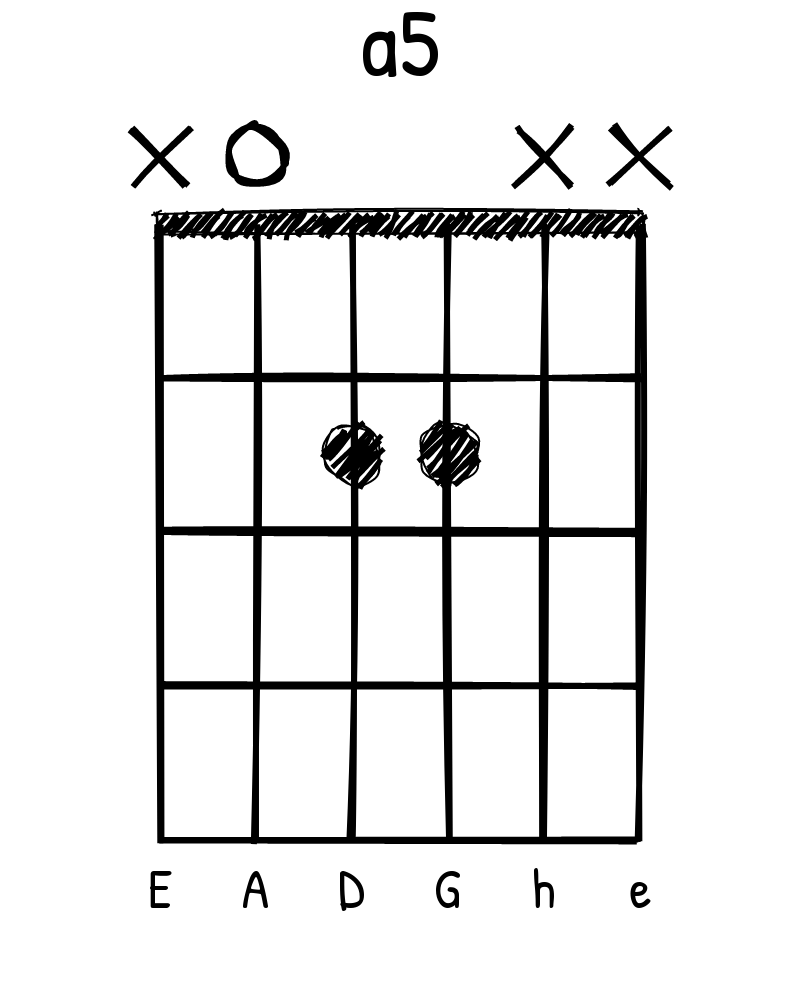
\includegraphics[height=3.5cm]{images/a5.png} \\
      \vspace{0.6cm}
      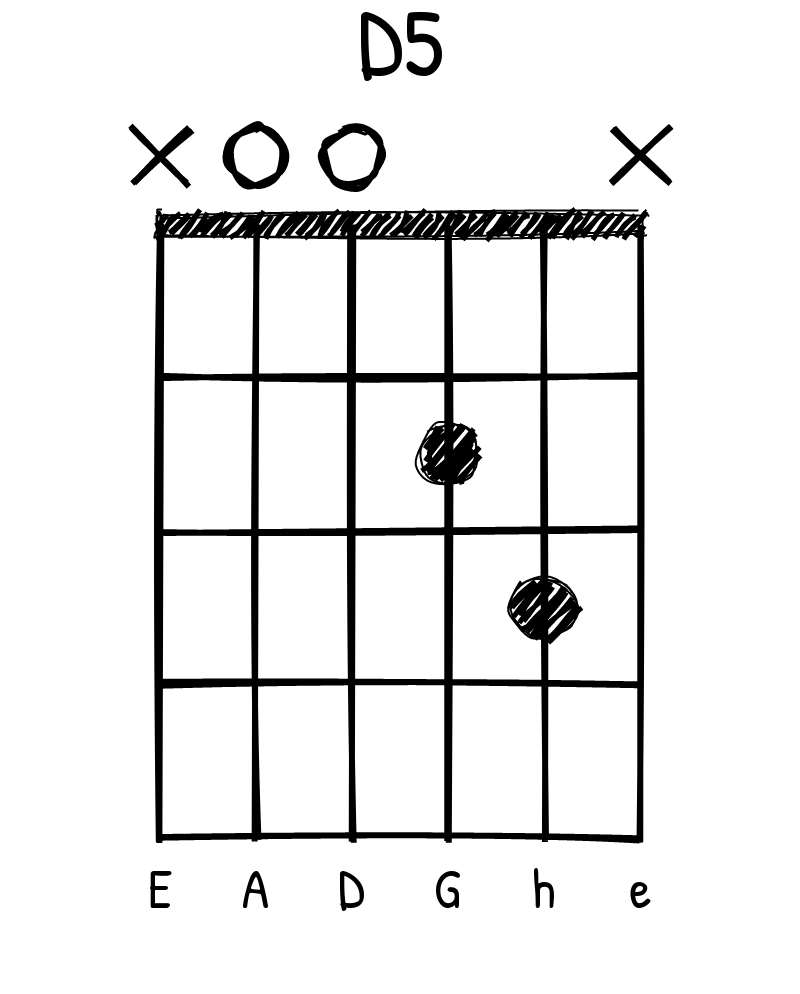
\includegraphics[height=3.5cm]{images/D5.png}
    \end{center}
    \end{multicols}
\end{song}


\newpage
\begin{song}{title={Premium Boy (Somebody That I Used To Know)}, music={Gotye}, interpret={808 Squad}}
\begin{multicols}{2}
    \small
    \begin{intro}
        \writechord{d} \writechord{C} \writechord{d} \writechord{C} $\times 4$
    \end{intro}
    \begin{verse}
        ^{d}Now and ^{C}then I think of ^{d}when we ^{C}were toge^{d}ther ^{C} ^{d} ^{C} \\
        ^{d} Like when you ^{C}said you felt so ^{d}happy ^{C}you could di^{d}e ^{C} ^{d} ^{C} \\
        ^{d} Told my^{C}self that you were ^{d}right for ^{C}me \\
        ^{d} But felt so ^{C}lonely in your ^{d}company ^{C} \\
        ^{d} But that was ^{C}love and it's an ^{d}ache I ^{C}still remem^{d}ber ^{C} ^{d} ^{C}
    \end{verse}
    \begin{interlude}
        \writechord{d} \writechord{C} \writechord{d} \writechord{C} $\times 4$
    \end{interlude}
    \begin{verse}
        You can get addicted to a certain kind of sadness \\
        Like resignation to the end, always the end \\
        So when we found that we could not make sense \\
        Well you said that we would still be friends \\
        But I'll admit that I was glad it was over
    \end{verse}
    \begin{chorus}
        ^{d} Bo ^{C}Michał to jest ^{B}premium ^{C}boy \\
        ^{d} Pije ^{C}kawę z mlekiem ^{B}sojowym gar^{C}dzi normal^{d}ną \\
        ^{C}Gardzi także ^*{B}herba ^{C}tą \\
        ^{d}Chyba że po^{C}słodzi cukrem ^*{B}trzcino ^{C}wym \\
        ^{d} Michał ^{C}to jest taki ^{B}premium ^{C}boy \\
        ^{d} Na jego ^{C}chlebie możesz ^{B}znaleźć tylko ^{C}  majo^{d}nez \\
        ^{C}Kiedyś zgłupiał ^{B}włączył ^{C}jazz \\
        ^{d}Potem wszedł na ^{C}łóżko i ze^{B}rzygał ^{C}się \\
        |: (bo Mi^{d}chał ^{C}--- to ^{B}premium bo^{C}y) | \\
        | ^{d}Każdy wie, że ^{C}Michał to jest ^{B}premium ^{C}boy :| \\
    \end{chorus}
    \begin{interlude}
        \writechord{d} \writechord{C} \writechord{d} \writechord{C} $\times 4$
    \end{interlude}
\end{multicols}
\end{song}


\newpage
\begin{song}{title={Riptide}, music={Vance Joy}}
    \small
    \begin{intro}
        \writechord{a} \writechord{G} \writechord{C} \writechord{C} $\times 2$
    \end{intro}
    \begin{verse}
        ^{a}I was scared of de^{G}ntists and the d^{C}ark \\
        ^{a}I was scared of ^{G}pretty girls and ^{C}starting conversations \\
        A^{a}ll my fri^{G}ends are turning ^{C}green \\
        You\tqs{}re the ^{a}magician\tqs{}s as^{G}sistant in their ^{C}dreams \smallskip

        A^{a}woo, ^{G}ooo, ^{C}ooo \\
        A^*{a}aa-- a^{G}ah, and they ^{C}come unstuck
    \end{verse}
    \begin{chorus}
        ^{a}Lady, ^{G}running down to the ^{C}riptide \\
        Taken away to the ^{a}dark side, ^{G}I wanna be your ^{C}left hand man \\
        I ^{a}love you ^{G}when you\tqs{}re singing that ^{C}song, and \\
        I got a lump in my ^{a}throat, \tqs{}cause ^{G}you\tqs{}re gonna sing the wor^{C}ds wrong
    \end{chorus}
    \begin{verse}
        Here\tqs{}s this movie that I think you\tqs{}ll like \\
        This guy decides to quit his job and heads to New York City \\
        This cowboy\tqs{}s running from himself \\
        And she\tqs{}s been living on the highest shelf \smallskip

        Awoo, ooo, ooo \\
        Aaa--aah, and they come unstuck
    \end{verse}
    \begin{chorus}
        Lady, running down to the riptide\ldots
    \end{chorus}
    \begin{riff}
        \writechord{D4}--\writechord{E4}--\writechord{C4}--\writechord{G4} -- \writechord{C4}--\writechord{E4} $\times 4$
    \end{riff}
    \begin{interlude}
        ^{a}I just wanna, I just wanna kn^{G}ow \\
        ^{C}If you\tqs{}re gonna, if you\tqs{}re gonna st^{F}ay \\
        ^{a}I just gotta, I just gotta kn^{G}ow \\
        ^{C}I can\tqs{}t have it, I can\tqs{}t have it ^{F}any other way \smallskip \\
        I s^{a}wear she\tqs{}s ^{G}destined for the ^{C}screen \\
        Cl^{a}osest thing to ^{G}Michelle Pfeiffer ^{C}that you\tqs{}ve ever seen, oh
    \end{interlude}
    \begin{chorus}
        Lady, running down to the riptide\ldots $\times 2$
    \end{chorus}
\end{song}


\newpage
\small
\begin{song}{title={Scenariusz dla moich sąsiadów}, music={Myslovitz}}
    \begin{intro}
        \writechord{A} \\
        \writechord{G} \writechord{F} \writechord{E}
    \end{intro}
    \begin{verse}
          ^{A} Kiedy powrócisz już ^{G} ja będę cz^{F}ekał ^{E} \\
        Ulicą pójdę wzdłuż kupię gazetę \\
        Zabiorę z sobą psa usiądę na ławce \\
        Skończę scenariusz by gotowy był \\
        Wieczorem
    \end{verse}
    \begin{chorus}
        ^{C}Wieczorem pr^{e}zed mym domem \\
        ^{F} Wystawię ekran i wyświetlę film ^{C} \\
        Coś o mnie i ^{e}o tobie \\
        ^{F} Będę leczył chore sąsiadów sny ^{C} ^{e}
    \end{chorus}
    \begin{interlude}
        \textit{akordy jak w zwrotce} \\
        oo oooo oo o o \\
        o oooo ooo ooo $\times 2$
    \end{interlude}
    \begin{verse}
        Z nieba przyleciał mój wielki przyjaciel \\
        Kiedy lądował ja jadłem kanapkę \\
        Wyśnił że chyba jest chorym człowiekiem \\
        Usiądź wygodnie i nie martw się \\
        Bo wieczorem
    \end{verse}
    \begin{chorus}
        Wieczorem przed mym domem\ldots
    \end{chorus}
    \begin{interlude}
        oo oooo oo o o \\
        o oooo ooo ooo $\times 2$
    \end{interlude}
    \begin{chorus} 
        Wieczorem przed mym domem\ldots $\times 2$
    \end{chorus}
\end{song}


\newpage
\begin{song}{title={Jest już za późno}, lyrics={Edward Stachura}, music={Stare Dobre Małżeństwo}}
    \begin{intro}
        \writechord{C} \writechord{F} \writechord{C} \writechord{F} 
    \end{intro}
    \begin{verse}
        ^{C}Jeszcze zdążymy w dżu^{d}ngli ludzkości ^{C}siebie odnaleźć ^{F} ^{C} \\
        ^{F} Tęskność zawr^{C}otna przybliża n^{d}as ^{G} \\
        ^{C}Zbiegną się wreszcie to^{d}ry sieroce n^{C}aszych dwóch planet ^{F} ^{C} \\
        ^{F} Cudnie spokr^{C}ewnią się ciała n^{d}am ^{G}
    \end{verse}    
    \begin{chorus}
        ^{e}Jest już za późno \\
        ^{F}Nie jest za późno \\
        ^{e}Jest już za późno \\
        ^{F}Nie jest za późno \\
        ^{e}Jest już za późno \\
        ^{F}Nie jest za ^{G}późno $\times 2$
    \end{chorus}
    \begin{verse}
        Jeszcze zdążymy tanio wynająć małą mansardę \\
        Z oknem na rzekę lub też na park \\
        Z łożem szerokim, piecem wysokim, ściennym zegarem \\
        Schodzić będziemy codziennie w świat 
    \end{verse}
    \begin{chorus}
        Jest już za późno\ldots $\times 2$
    \end{chorus}
    \begin{verse}
        Jeszcze zdążymy naszą miłością siebie zachwycić \\ 
        Siebie zachwycić i wszystko w krąg \\
        Wojna to będzie straszna, bo czas nas będzie chciał zniszczyć \\
        Lecz nam się uda zachwycić go
    \end{verse}
     \begin{chorus}
        Jest już za późno\ldots $\times 2$
    \end{chorus}
\end{song}


\newpage
\normalsize
\begin{song}{title={Space Oddity}, music={David Bowie}}
\begin{multicols}{2}
	\begin{intro}
	    \writechord{Fmaj7} \writechord{e} $\times 2$
	\end{intro}
    \begin{verse}    
        ^{C} Ground Control to Major To^{e}m \\
        ^{C} Ground Control to Major To^{e}m \\
        ^{a} Take your pro^{a/G}tein pills and \\
        P^{D/F#}ut your helmet on \\
        ^{C} Ground Control to Major To^{e}m \\
        \textit{(ten, nine, eight, seven, six)} \\
        ^{C} Commencing countdown, engines o^{e}n \\
        \textit{(five, four, three)}
         \\
        ^{a} Check igni^{a/G}tion and may \\
        ^{D/F#}God's love be with you \\
        \textit{(two, one, liftoff)} \\ \\
        \textit{6 taktów przerwy, \textbf{narastający chaos}} 
    \end{verse}
    \begin{verse}    
        ^{C}This is Ground Control to Major T^{E}om \\
        You've really made the gr^{F}ade \\
        And the pa^{f}pers want to kn^{C}ow whose shirts you w^{F}ear \\
        Now it's t^{f}ime to leave the cap^{C}sule if you d^{F}are \\
        Th^{C}sis is Major Tom to Ground Co^{E}ntrol \\
        I'm stepping through the do^{F}or \\
        And I'm fl^{f}oating in a m^{C}ost peculiar w^{F}ay \\
        And the st^{f}ars look very dif^{C}ferent tod^{F}ay 
    \end{verse}
    \begin{chorus}
        For he^{Fmaj7}re \\
        Am I si^{e}tting in a tin can \\
        ^{Fmaj7}Far above the wo^{e}rld \\
        ^{B}Planet Earth is b^{a}lue \\
        And there's n^{G}othing I can ^{F}do
    \end{chorus}
    \begin{interlude}
        |: C F G \\
        A A :|  \\
        \writechord{Fmaj7} e \\
        A C \\
        D E \\
    \end{interlude}
    \begin{verse}
        ^{C}Though I'm past one hundred thousand mi^{E}les \\
        I'm feeling very st^{F}ill \\
        And I th^{f}ink my spaceship kn^{C}ows which way to ^{F}go \\
        Tell my w^{f}ife I love her ve^{C}ry much she kn^{F}ows \\
    \end{verse}
    \begin{interlude}
        ^{G}Ground Control to ^{E7}Major Tom \\
        Your ^{a}circuit's dead, there's ^{a/G}something wrong \\
        Can you ^{D}hear me, Major Tom? \\
        Can you ^{C}hear me, Major Tom? \\
        Can you ^{G}hear me, Major Tom? \\
        Can you 
    \end{interlude}
    \begin{chorus}
        ^{Fmaj7}Here am I ^{e}floating 'round my tin can \\
        ^{Fmaj7}Far above the ^{e}moon \\
        ^{B}Planet Earth is ^{a}blue \\
        And there's ^{G}nothing I can ^{F}do
    \end{chorus}
\end{multicols}
\end{song}


\newpage
\begin{song}{title={Sunny Afternoon}, music={The Kinks}}
    \begin{intro}
        \begin{tabular}{l l l l}
            \writechord{d} & \writechord{d/C} & \writechord{d/Cb} & \writechord{d/B} \\
            \writechord{A7} &  \writechord{A7/G} & \writechord{A7/F} & \writechord{A7/E} $\times 2$
        \end{tabular}
    \end{intro}
    \begin{verse}
        The ^{d}taxman\tqs{}s taken ^{C}all my dough \\
        And ^{F}left me in my ^{C}stately home \\
        ^{A}Lazin\tqs{} on a sunny aftern^{d}oon \smallskip \\
        And I can\tqs{}t ^{C}sail my yacht \\
        He\tqs{}s ^{F}taken every^{C}thing I\tqs{}ve got \\
        ^{A}All I\tqs{}ve got\tqs{}s this sunny aftern^{d}oon
    \end{verse}
    \begin{chorus}
        ^{D}Save me, save me, save me from this squ^{G}eeze \\
        I got a ^{C}big fat momma, tryin\tqs{} to break ^{F}me ^{A7} \\
        And I ^{d}love to live so ^{G}pleasantly \\
        ^{d}Live this life of l^*{G}uxu ^{C}ry \\
        ^{F}Lazin\tqs{} on a ^{A7}sunny aftern^{d}oon ^{d/C} ^{d/Cb} ^{d/B} \\
        In the ^*{A7}summert ^{A7/G}ime ^{A7/F} ^{A7/E} \\
        In the ^*{d}summert ^{d/C}ime ^{d/Cb} ^{d/B} \\
        In the ^*{A7}summert ^{A7/G}ime ^{A7/F} ^{A7/E}
    \end{chorus}
    \begin{verse}
        My girlfriend\tqs{}s run off with my car \\
        And gone back to her ma and pa \\
        Telling tales of drunkenness and cruelty \smallskip \\
        Now I\tqs{}m sitting here \\
        Sipping at my ice cold beer \\
        Lazin\tqs{} on a sunny afternoon
    \end{verse}
    \begin{chorus}
        Help me, help me, help me sail away \\
        Well, give me two good reasons, why I ought to stay \\
        \tqs{}Cause I love to live so pleasantly \\
        Live this life of luxury \\
        Lazin\tqs{} on a sunny afternoon \\
        In the summertime, in the summertime \\
        In the summertime \medskip

        Save me, save me, save me from this squeeze\ldots
    \end{chorus}
\end{song}


\newpage
\begin{song}{title={To nie ptak}, music={Goran Bregović}, lyrics={Kayah}}
    \begin{multicols}{2}
    \begin{intro}
        /textit{(bałkańskie plumkanie na gitarze)} \\
        \writechord{a} \writechord{E} \writechord{a} \writechord{a} \\
    \end{intro}
    \begin{verse}
        W ko^{a}lorowej sukien^{C}eczce krząta s^{a}ię ---^{E}--- \\
        ^{a}Raz po raz odwraca gł^{C}owę, uśmiech śl^{a}e ---^{E}--- \\ 
        ---^{a}---  Mó^{E}głbyś przysiąc, ż^{a}e \\
        Widziałeś wcz^{E}oraj skrzydła j^{a}ej \\
        Jak je chowa^{G}ła pod suki^{F}enką, lecz ona \\
        T^{a}o   ni^{C}e   pt^{d}ak \\
    \end{verse}
    \begin{chorus}
        Czy nie widzisz ---^{a}--- ---^{d}--- ---^{a}--- \\
        To n^{d}ie jest pt^{a}ak  ---^{d}--- ---^{a}---  \\
        Ona t^{d}o nie pta^{a}k ---^{d}--- ---^{a}--- \\
        To n^{d}ie jest pt^{a}ak czy nie ^{d}widzi--s^{a}z \\ \\ \\
        \writechord{a} \writechord{E} \writechord{a} \writechord{a} \\
        \columnbreak
    \end{chorus}
    \begin{verse}
        Kocham ciebie mówi jej każdy mały ruch \\
        Lecz ty wśród kolorowych falban szukasz piór \\
        Bo jesteś pewien że \\
        Wczoraj widziałeś skrzydeł cień \\
        Dlatego klatkę zbudowałeś, lecz ona \\ 
        To nie ptak \\
    \end{verse}
    \begin{chorus}
        Czy nie widzisz \\
        To nie jest ptak \\
        Ona to nie ptak \\
        To nie jest ptak czy nie widzisz \\
    \end{chorus}
    \begin{interlude}
        O^{a}j dana oj dana ooj daj da^{d}j daj \\
        Ooooj da^{E}aaj da^{a}aaj --^{a}-- --^{d}-- --^{a}-- --^{d}-- $\times 2$
    \end{interlude}
    \begin{verse}
        Tego dnia, gdy ciemność skradnie serce ci \\
        Ona w oknie będzie śmiać się lecz przez łzy \\
        Rozpuści czarność włosów i \\
        Zmieniona w kruka skoczy by \\
        Za chwilę oknem tym powrócić tu, lecz jako \\
        Rajski ptak \\
    \end{verse}
    \begin{chorus}
        Rajski ptak bo tak chciałeś \\
        Jako rajski ptak \\
        Rajski ptak \\
        Jako rajski ptak bo tak chciałeś \\
    \end{chorus}
    \begin{interlude}
        Oj dana oj dana ooj daj daj daj \ldots
    \end{interlude}
    \end{multicols}
\end{song}


\newpage
\begin{song}{title={Trudno nie wierzyć w nic}, music={Raz Dwa Trzy}} 
    \begin{intro}
        \begin{tabular}{l l l l l}
            \writechord{e} & \writechord{G/D}   & \writechord{Cmaj7} & \writechord{Hsus4} \\
            \writechord{e} & \writechord{F#/B}  & \writechord{a5}    & \writechord{H}     \\
            \writechord{e} & \writechord{G/D}   & \writechord{Cmaj7} & \writechord{Hsus4} \\
            \writechord{C} & \writechord{Dsus2} & \writechord{e5}    &                    & $\times 2$
        \end{tabular}
    \end{intro}
    \begin{multicols}{2}
    \begin{verse}
        ^{e} ^{G/D}Zapyta Bóg ^{C(5-)} w swym ^{H}niebie \\
        ^{e} Co ^{G/D}dałem Mu, ^{C(5-)} od ^{H}siebie \\
        ^{e} ^{G/D}Wierzyłem i ^{C(5-)} ^{H}kochałem \\
        ^{e} I ^{G/D}byłem tym, ^{C(5-)} kim ^{H}chciał bym ^{C}był \smallskip \\
        I ż^{D}yłem jak, ^{C}chciał bym żył \\
        I ^{D}byłem, kim mi^{H}ałem być
    \end{verse}
    \begin{interlude}
        \textit{(intro)} $\times 1$
    \end{interlude}
    \begin{verse}
        Odpowiem Mu od siebie \\
        Że spłacę dług tym lepiej \\
        Tym bardziej, bo wiedziałem \\
        Co znaczy, że nadziei brakowało mi \medskip \\
        ^{C} I ^{D}kilku chwil, kilku ^{G}dobrych chwil ^{C} \\
        Może powie, ^{a}to niepotr^{H}zebne słowa
    \end{verse}
    \begin{chorus}
        ^{e} ^{G/D} Trudno nie w^{C(5-)}ierzyć w nic ^{H} \\
        Trudno nie wierzyć w nic \\
        Trudno nie wierzyć w nic \\
        Trudno nie wierzyć w nic
    \end{chorus}
    \begin{solo}
        C D $\times 8$
    \end{solo}
    \begin{verse}
        Zapyta Bóg w swym niebie \\
        Jak spłacę dług --- ja nie wiem \\
        Wierzyłem i kochałem \\
        I byłem tym, kim chciał bym był
    \end{verse}
    \begin{chorus}
        Trudno nie wierzyć w nic \\
        Trudno nie wierzyć w nic
    \end{chorus}
    \begin{outro}
        \textit{(intro)} $\times 1$
    \end{outro}
    \vfill\null\columnbreak{}
    \begin{center}
        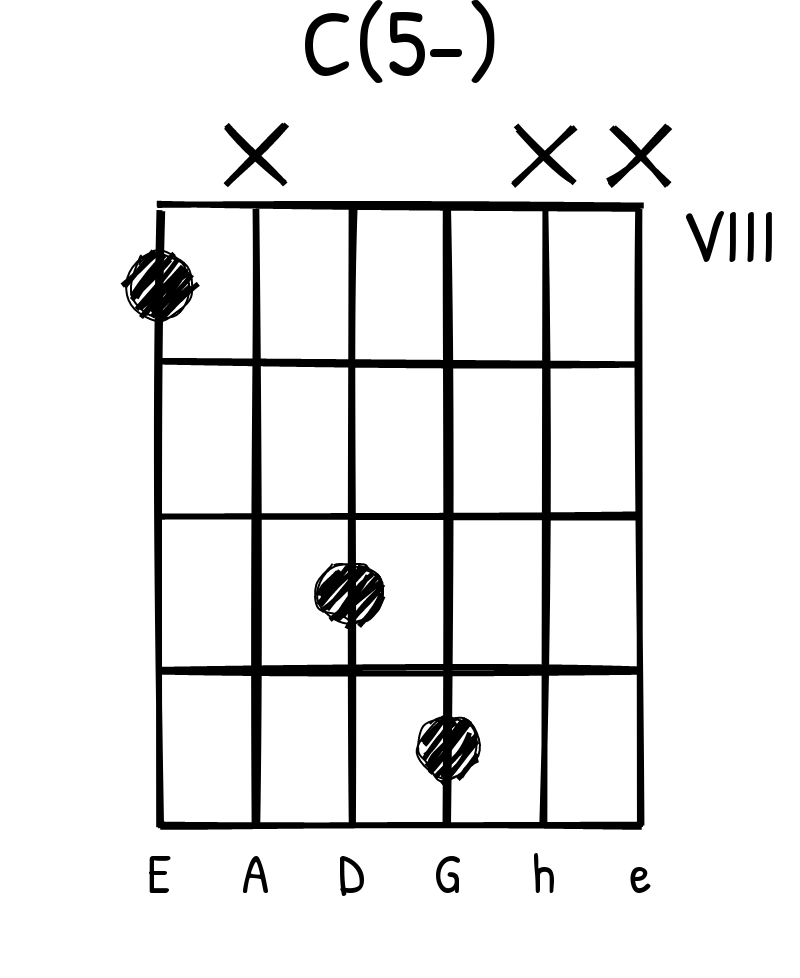
\includegraphics[height=3.5cm]{images/C5dim.png}
    \end{center}
    \end{multicols}
\end{song}


\newpage
\begin{song}{title={Warszawa}, music={T.Love}, capo=2}
    \begin{intro}
        \writechord{D} \writechord{G} $\times 2$
    \end{intro}
    \begin{multicols}{2}
    \begin{verse}
        Za ^{A}oknem zimowo zaczyna się dzień \\
        Za^{h}czynam kolejny dzień ż^{G}ycia \\
        Wyg^{A}lądam przez okno, na oczach mam sen \\
        A ^{h}Grochów się budzi z prze^{G}picia \medskip

        Wypity alkohol uderza w tętnice \\
        Autobus tapla się w śniegu \\
        Zza szyby oglądam betonu stolicę \\
        Już jestem na drugim jej brzegu
    \end{verse}
    \begin{chorus}
        Gdy ^{D}patrzę w twe ^{A}oczy zmę^{G}czone jak moje \\
        To ^{D}kocham to ^{A}miasto zmę^{G}czone jak ja \\
        Gdzie ^{D}Hitler i Sta^{A}lin zro^{G}bili, co swoje \\
        Gdzie ^{D}wiosna spa^{A}liną odd^{G}ycha
    \end{chorus}
    \begin{interlude}
        \writechord{D} \writechord{G} $\times 2$
    \end{interlude}
    \vfill\null\columnbreak{}
    \begin{verse}
        Krakowskie Przedmieście zalane jest słońcem \\
        Wirujesz jak obłok, wynurzasz się z bramy \\
        A ja jestem głodny, tak bardzo głodny \\
        Kochanie, nakarmisz mnie snami \medskip

        Zielony Żoliborz, pieprzony Żoliborz \\
        Rozkwita na drzewach, na krzewach \\
        Ściekami z rzeki kompletnie pijany \\
        Chcę krzyczeć, chcę ryczeć, chcę śpiewać
    \end{verse}
    \begin{chorus}
        Gdy patrzę w twe oczy zmęczone jak moje\ldots \smallskip

        \writechord{A} \writechord{h} \smallskip

        Gdy patrzę w twe oczy zmęczone jak moje\ldots
    \end{chorus}
    \begin{interlude}
        \writechord{A} \writechord{A} \writechord{h} \writechord{G} $\times 4$ \textit{(jak w zwrotce)} \medskip \\
        \writechord{D} \writechord{A} \writechord{D} \\
        (\writechord{A})\writechord{D} \writechord{G} \writechord{A} \\
        \writechord{D} \writechord{A} \writechord{D} \medskip \\
        \writechord{D} \writechord{A} \writechord{D} \\
        (\writechord{A})\writechord{D} \writechord{G} \writechord{A} \\
        \writechord{G}
    \end{interlude}
    \begin{verse}
        Jesienią zawsze zaczyna się szkoła \\
        A w knajpach zaczyna się picie \\
        Jest tłoczno i duszno, olewa nas kelner \\
        I tak skończymy o świcie \medskip

        Jesienią zawsze myślę o latach \\
        Tak starych, jak te kamienice \\
        Jesienią o zmroku przechodzę z tobą \\
        Przez pełne kasztanów ulice
    \end{verse}
    \begin{chorus}
        I patrzę w twe oczy zmęczone jak moje \\
        I kocham to miasto zmęczone jak ja \\
        Gdzie Hitler i Stalin zrobili, co swoje \\
        Gdzie wiosna spaliną oddycha $\times 2$
    \end{chorus}
    \begin{outro}
        \writechord{A} \writechord{D}
    \end{outro}
    \end{multicols}
\end{song}


\newpage
\begin{song}{title={Wymyśliłem ciebie}, music={Dżamble}, interpret={Andrzej Zaucha}}
    \begin{intro}
    \writechord{C} \writechord{a} \writechord{e/H} \writechord{H}
    \end{intro}
    \begin{multicols}{2}
    \begin{verse}
        ^{e}Dzisiaj na^{e7/D}gle ^{C}wymyśliłem C^{H}iebie  \\
        ^{e}Twoje i^{e7/D}ię ^{C}zadźwięczało w^{H}e mnie  \\
        ^{a}Choć ^{a5+}tyle ^{a6}innych jes^{a7}t  \\
        ^{a}Znam ^{a5+}tylko ^{a6}jego dźw^{a7}ięk  \\
        Do mnie m^{e}ów najłagodni^{e7/D}ej \\
        Jak tylko ^{C}Ty potr^{H7}afisz \\
        ^{e}I podaj rękę spł^{e7/D}oszoną \\
        ^{C}Szczęściem ^{Hsus4}nagły^{H7}m \\
    \end{verse}
    \begin{chorus}
        ^{e}Dla ciebie usta ^{Hsus4}mo - j^{H7}e \\
        ^{H7/F#}I ciepło moich dł^{G7+5+}o - n^{e}i \\
        A p^{F/A}otem przyjdą n^{e/H}oce \\
        Jak psy wi^{F/A}erne - p^{H}od nasz dom \\ \\
        \writechord{C} \writechord{a} \writechord{e/H} \writechord{H} \\
    \end{chorus}
    \begin{solo}
        \writechord{e} \writechord{e7/D} \writechord{C} \writechord{H7} $\times 2$
    \end{solo}
    \begin{verse}
        ^{e}Jaką dr^{e7/D}ogę ^{C}wybierzemy r^{H}azem  \\
        ^{e}Spłonął wi^{e7/D}eczór ^{C}w horyzoncie gw^{H}iazdą \\
        ^{a}Ta gwi^{a5+}azda św^{a6}ieci z^{a7}nów \\
        ^{a}Nad j^{a5+}edną z na^{a6}szych dró^{a7}g  \\
        W oczy p^{e}atrz najłagodni^{e7/D}ej  \\
        Jak tylko ^{C}Ty potr^{H7}afisz \\
        ^{e}I całuj wargi spł^{e7/D}oszone \\
        ^{C}Szczęściem ^{Hsus4}nagły^{H7}m \\
    \end{verse}
    \begin{chorus}
        ^{e}Dla ciebie usta ^{Hsus4}mo - j^{H7}e \\
        ^{H7/F#}I ciepło moich dł^{G7+5+}o - n^{e}i \\
        A p^{F/A}otem przyjdą n^{e/H}oce \\
        Jak psy wi^{F/A}erne - p^{H}od nasz dom \\ \\
        \writechord{C} \writechord{a} \writechord{e/H} \writechord{H} \\
    \end{chorus}
    \end{multicols}
\end{song}


\newpage
\begin{song}{title={Zanim pójdę}, music={Happysad}}
    \begin{intro}
        \writechord{a} \writechord{d7} \writechord{e7} $\times 4$
    \end{intro}
    \begin{verse}
        Ile ^{a}jestem ^{d7}ci ^{e7}winien \\
        Ile poli^{a}czyłaś mi za ^{d7}swą ^{e7}przyjaźń \\
        Ale kiedy ^{a}wszystko już od^{d7}dam, ^{e7}czy \\
        |: Będziesz szczęś^{a}liwa i wol^{d7}na, ^{e7}czy\ldots :| \smallskip \\
        |: Ale zanim ^{a}pójdę ^{d7} ^{e7} :| \\
        Ale zanim ^{a}pójdę, chciał^{d7}bym po^{e7}wiedzieć ci, że\ldots
    \end{verse}
    \begin{chorus}
        ^{a}Miłość, to nie plu^{d}szowy ^{e}miś \\
        Ani ^{a}kwiaty, to też nie ^{d}diabeł ro^{e}gaty \\
        Ani ^{a}miłość, kiedy ^{d}jedno ^{G}płacze \\
        A ^{C}drugie po nim ^{F} skacze \medskip \\
        Miłość, to żaden film w żadnym kinie \\
        Ani róże, ani całusy małe duże \\
        Ale miłość --- kiedy jedno spada w dół \\
        Drugie ciągnie je ku górze
    \end{chorus}
    \begin{chorus*}
        \writechord{a} \writechord{d7} \writechord{e7} $\times 4$
    \end{chorus*}
    \begin{verse}
        Ile jestem ci winien \\
        Ile policzyłaś mi za swą przyjaźń \\
        Ile były warte nasze słowa \\
        |: Kiedy próbowaliśmy wszystko od nowa :| \smallskip \\
        |: Ale zanim pójdę :| \\
        Ale zanim pójdę, chciałbym powiedzieć ci, że\ldots
    \end{verse}
    \begin{chorus}
        Miłość, to nie pluszowy miś\ldots
    \end{chorus}
    \begin{interlude}
        \writechord{a} \writechord{d7} \writechord{e7} $\times 8$ \medskip \\
        |: Ale zanim pójdę :| \\
        Ale zanim pójdę, chciałbym powiedzieć ci, że\ldots
    \end{interlude}
    \begin{chorus}
        Miłość, to nie pluszowy miś\ldots$\times 2$
    \end{chorus}
    \begin{chorus*}
        \writechord{a} \writechord{d7} \writechord{e7} $\times 4$ \\
        \writechord{C}
    \end{chorus*}
\end{song}



\chapter{Polska na Eurowizji}
\begin{center}
    
\includegraphics[width=0.4\textwidth]{images/Eurovision-Logo.png}
\end{center}
\pagestyle{pop}
\newpage
\begin{song}{title={To nie ja}, music={Stanisław Syrewicz}, lyrics={Jacek Cygan}, interpret={Edyta Górniak}}
    \begin{intro}
    \writechord{A} \writechord{h7/A} \\ 
    \writechord{A} \writechord{h7/A}
    \end{intro}
    \begin{multicols}{2}
    \begin{verse}
        ^{A}Świat mój tak zwycz^{h7/A}ajny \\
        Pod n^{A}iebem biało-cz^{h7/A}arnym  \\
        L^{A}udzie s^{A/C#}ą wyci^{D}ęci z szarych str^{h}on \\
        Ze środka ks^{E7sus4}iąg \\
    \end{verse}
    \begin{verse}
        ^{A}Piękni są z rom^{h7/A}ansu tła  \\
        Zmę^{A}czeni tylko z g^{h7/A}azet  \\
        A j^{A/C#}a jestem bi^{D}ałą, czystą k^{h}artką \\
        Pośró^{G}d Wa^{A}s \\
    \end{verse}
    \begin{chorus}
        To nie ja byłam E^{D}wą \\
        To nie ja skradłam ^{h}niebo  \\
        Chociaż dosyć mam ł^{G}ez, moich łez, tylu łez  \\
        Jestem p^{E/G#}o to, by ko^{A}chać mnie  \\
        To nie ja byłam E^{D}wą, to nie ja skradłam ni^{h}ebo  \\
        Nie dodawaj mi w^{e7}in, to nie ja, to nie j^{D/F#}a  \\
        Nie j^{Asus4}a -- jestem Ew^{h7}ą \\
        \\ \writechord{E7sus4}  \\ \\
    \end{chorus}
    \begin{verse}
        ^{A}Niebo wieje chł^{h7/A}odem  \\
        ^{A/C#}Piekło kłania się ^{D}ogniem do stóp \\
        A j^{A/C#}a, papier^{D}owa marion^{h}etka, musz^{G}ę gra^{A}ć  \\
    \end{verse}
    \begin{chorus}
        To nie ja byłam ^{D}Ewą \\
        To nie ja skradłam ^{h}niebo  \\
        Chociaż dosyć mam ^{G}łez, moich łez, tylu łez  \\
        Jestem p^{E7/G#}o to, by ko^{A}chać, wiem \\
    \end{chorus}
    \begin{interlude}
        Zanim w popiół się zmi^{e}enię, chcę być wielkim pł^{e7/D}omieniem \\
        Chcę się wzbić ponad ś^{A7}wiat, hen, ogrzać niebo ma^{D}rzeniem oooo^{H7}o  \\
    \end{interlude}
    \begin{solo}
        \writechord{E} \writechord{Emaj7/D#} \writechord{c#} \writechord{E/H} \\
        \writechord{A} \writechord{Amaj7/G#} \writechord{f#7} \writechord{H7} \\
        \writechord{E} \writechord{Emaj7/D#} \writechord{c#} \writechord{E/H} \\
    \end{solo}
    \begin{interlude}
        To nie j^{f#7}a pragnę zł^{E/G#}a  \\
        Nie j^{A}a! \\
    \end{interlude}
    \begin{outro}
        \writechord{C} \writechord{D} \\
        \writechord{E}
    \end{outro}
    \end{multicols}
\end{song}



\chapter{Autorskie}
\begin{center}
    
\includegraphics[width=0.4\textwidth]{images/writing_hand.jpeg}
\end{center}
\pagestyle{autorskie}
\newpage
\begin{song}{title={Dzień Wojownika}, music={Ślad}}
    \normalsize
    \begin{multicols}{2}
    \begin{intro}
        \writechord{h7} \writechord{A6} \writechord{GΔ7} \writechord{f#7}
    \end{intro}
    \begin{verse}

	Po^{h7}wiedz mi,^{A6} jak wygląda dz^{GΔ7}ień ^{f#7} \\
	Dzień Wojown^{h7}ika? \\
	Twoja tw^{A6}arz tyle mówi m^{GΔ7}i, \\
	^{f#7}a ja nie umiem z niej cz^{h7}ytać ^{A6} \\
	I ten bl^{GΔ7}ask,^{f#7} blask w twoich ocz^{h7}ach, \\
	jak nagła z nieba r^{A6}osa \\
	Sk^{GΔ7}ąd bierzesz tyle s^{f#7}ił? \medskip

    \end{verse}
    \begin{chorus}
	Jak m^{h7}ożesz twierdzić, ż^{A6}e \\
	m^{GΔ7}oc w słabości d^{f#7}oskonali się? \\
	I wygr^{h7}ywać^{A6}, bo pomaga c^{GΔ7}i \\ 
	Kt^{f#7}oś, kogo nawet nie w^{h7}idać ^{f#7} ^{GΔ7} ^{A6} \medskip
    \end{chorus}
    \begin{verse}
	Po^{h7}wiedz mi,^{A6} jak się widzi św^{GΔ7}iat ^{f#7} \\
	Świat, gdy się w^{h7}ierzy? \\
	Taki św^{A6}iat jest tak obcy m^{GΔ7}i, \\
	^{f#7}a ty nie tracisz nadz^{h7}iei ^{A6} \\
	I ta m^{GΔ7}oc^{A6}, moc w twoim wn^{h7}ętrzu \\
	Nie gubisz nigdy s^{A6}ensu \\
	Sk^{GΔ7}ąd bierzesz t^{f#7}yle sił? \medskip
    \end{verse}
    \begin{chorus}
	Jak m^{h7}ożesz twierdzić, ż^{A6}e \\
	m^{GΔ7}oc w słabości d^{f#7}oskonali się? \\
	I wygr^{h7}ywać, ^{A6} bo pomaga c^{GΔ7}i \\ 
	Kt^{f#7}oś, kogo nawet nie w^{h7}idać ^{f#7} ^{GΔ7} ^{A6} $\times 2$
    \end{chorus}
    \end{multicols}
\end{song}



\newpage
\begin{song}{title={Niezapominajka}, music={Ślad}}
    \normalsize
    \begin{intro}
	\writechord{e} (dwa takty)
    \end{intro}
    \begin{verse}
        M^{e}ija przechodzień witryny sklepowe, mija kwiaciarnie i widzi, że \\
        Tak nienaganne, żywe bez wody, tak niezniszczalne ich życie jest. \medskip
    
        A t^{C}yle jest w n^{D}as z ż^{D}ycia kwiatu \\
        Błęk^{C}itną mam tw^{D}arz i w^{e}ieje wiatr \\
        Nie kł^{C}amię, że m^{D}am w^{D}iele czasu \\
        Pon^{C}iesie mnie t^{D}am, gdzie b^{h7sus}ędzie chciał \medskip
    \end{verse}
    \begin{chorus}
        T^{C}ak, j^{D}ak n^{e}iezapominajka, na tr^{C}aw ziel^{D}onym tl^{e}e \\ 
        Ch^{C}oc^{D}iaż życie to nie bajka, On n^{C}ie zap^{D}omni mn^{e}ie \\
        T^{C}ak, j^{D}ak n^{e}iezapominajka, na tr^{C}aw ziel^{D}onym tl^{e}e \\
        Ch^{C}oc^{D}iaż życie to nie bajka, On n^{C}ie zap^{D}omni mn^{h7sus}ie \medskip
    \end{chorus}
    \begin{verse}
        T^{e}utaj nie mamy witryny i sławy, pewnie uschniemy, gdy zniknie deszcz \\
        Zbyt delikatne są nasze płatki, ale nad nami niebo jest! \medskip

	A t^{C}yle jest w n^{D}as z ż^{D}ycia kwiatu... \\
    \end{verse}
    \begin{chorus}
        T^{C}ak, j^{D}ak n^{e}iezapominajka, na tr^{C}aw ziel^{D}onym tl^{e}e... \\
    \end{chorus}
    \begin{outro}
        A t^{C}yle jest w n^{D}as z ż^{D}ycia kwiatu \\
        Błęk^{C}itną mam tw^{D}arz i w^{e}ieje wiatr \\
        Nie kł^{C}amię, że m^{D}am w^{D}iele czasu \\
        Pon^{C}iesie mnie t^{D}am, gdzie b^{e}ędzie chciał 
    \end{outro}
\end{song}

\newpage
\begin{song}{title={Bouda}, music={Zofia Starosta, Mateusz Dorobek}}
    \begin{multicols}{2}
    \begin{verse}
        You got the Bouda, ^{D-7}bouda! \\
        You got the Honkers, ^{B7^{#9b13}}oh yeah! \\
        I got a Feeling, ^{E7^{#9b13}}for ya \\
        I wanna ^{A7^{#9b13}}hold you tight ^{D-7}   $\times 2$ \\
    \end{verse}
    \begin{chorus}
        Whe^{D7^{b9}}rever I s^{G-7}leep \\
        What ever I e^{D-9}at \\
        Whenever I take^{FMaj7} a shit or morning shower \\
        A^{Bb13}da Ada i^{A7^{#9b13}}n my Drea^{D-9}ms

        Whe^{D7^{b9}}rever I g^{G-7}o \\
        C^{G-7}hcę zoba^{A-}czyć j^{Bb}ą \\
        I nie jest ważne c^{B-7^{b5}}o kto inny gada \\
        W mo^{Bb13}je głowie t^{A7^{#9b13}}ylko Ada^{D-9}ms ^{Eb7^{#11}}
    \end{chorus}

    \begin{riff}
        \textit{Jam here in D blues scale and moove your bouda to this chonky chords:}\\
        |:
        \writechord{D-7} |
        \writechord{B7^{#9b13}} |
        \writechord{E7^{#9b13}} |
        \writechord{A7^{#9b13}} :|
        $\times 2137$
    \end{riff}

    \begin{verse}
        You got the Bouda, b^{D-7}ouda! \\
        You got the Honkers, o^{B7^{#9b13}}h yeah! \\
        I got a Feeling, f^{E7^{#9b13}}or ya \\
        I wanna h^{A7^{#9b13}}old you tight $\times 2$ \\
    \end{verse}
    \begin{chorus}
        Whe^{D7^{b9}}rever I s^{G-7}leep \\
        What ever I e^{D-9}at \\
        Whenever I take^{FMaj7} a shit or morning shower \\
        A^{Bb13}da Ada i^{A7^{#9b13}}n my Drea^{D-9}ms

        Whe^{D7^{b9}}rever I g^{G-7}o \\
        C^{G-7}hcę zoba^{A-}czyć j^{Bb}ą \\
        I nie jest ważne c^{B-7^{b5}}o kto inny gada \\
        W mo^{Bb13}je głowie t^{A7^{#9b13}}ylko Ada^{D-9}ms ^{Eb7^{#11}}
    \end{chorus}
\end{multicols}
\end{song}

\chapter{Legendy, opowieści, ciekawostki}
\begin{center}
    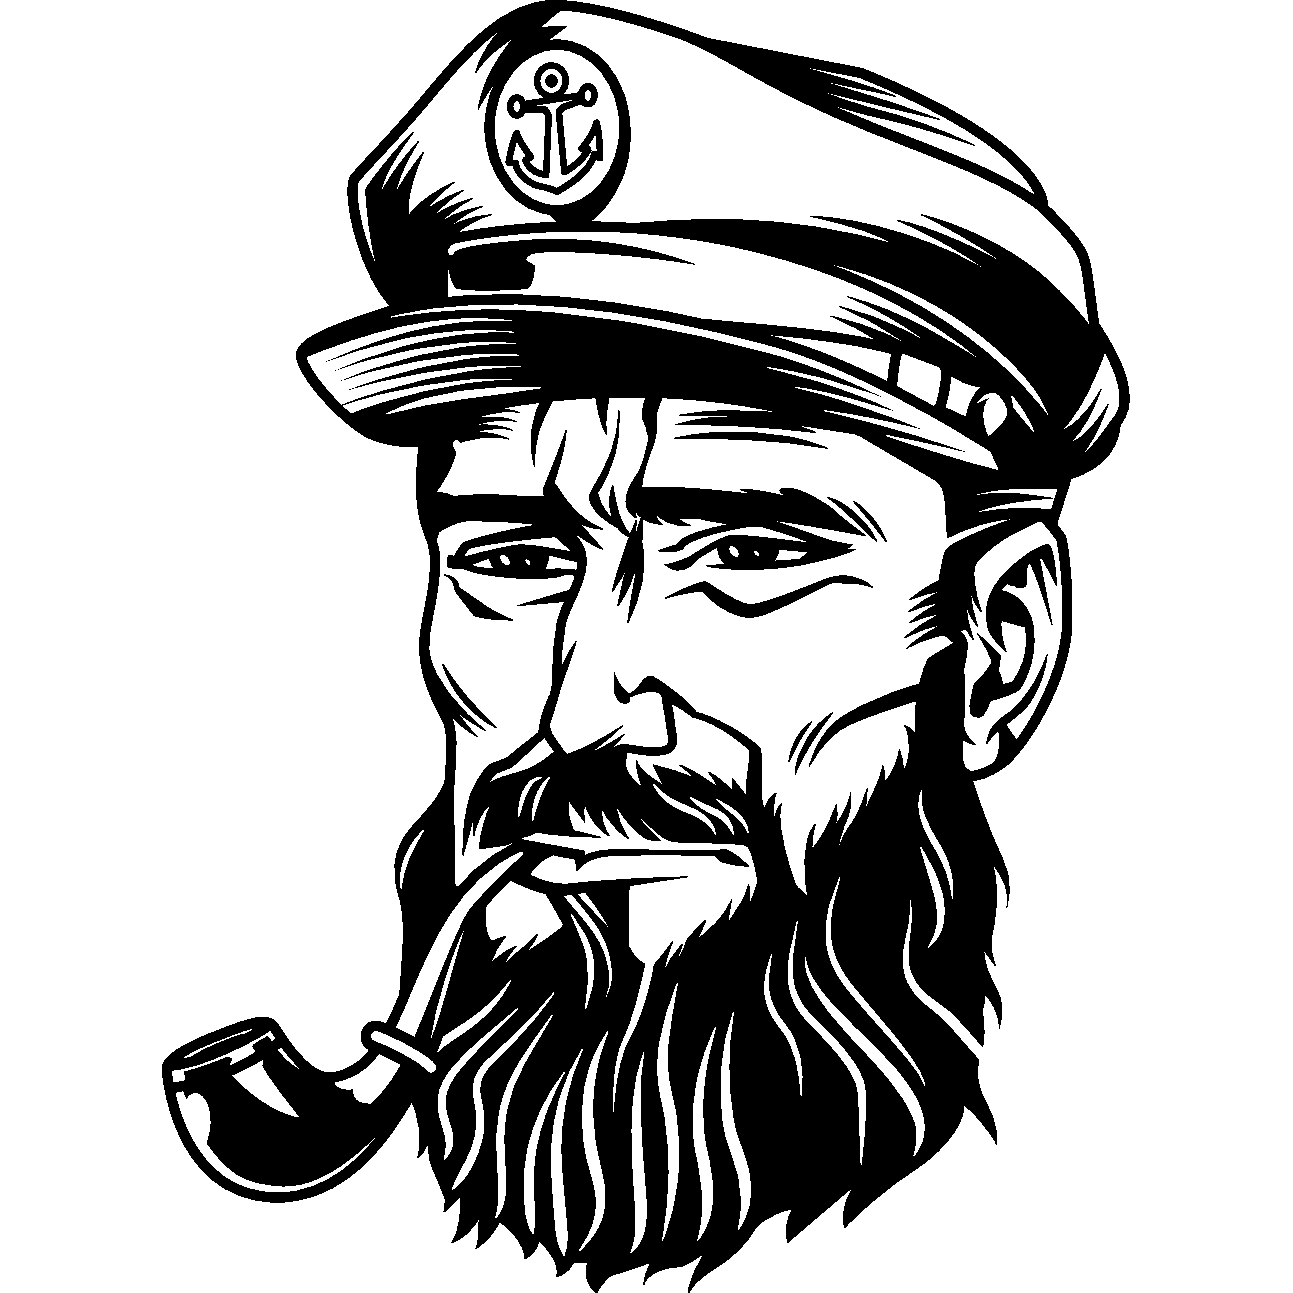
\includegraphics[width=0.4\textwidth]{images/bosman.png}
\end{center}
\pagestyle{legendy}
\newpage




% Ostatnia strona parzysta pusta, żeby nie było tekstu na odwrocie
\clearpage{\mbox{}\pagestyle{empty}\cleardoublepage}

\end{document}
